\section{キルヒホッフの法則と直流回路}

% ===========================================================================
%  再編（2026-09-24）：第4章 電磁気学 の第27回．
%  原本の 第34回「キルヒホッフの法則」の 34.4（ホイートストンブリッジ）と，
%  第35回「直流回路」の全体（35.1 コンデンサーの過渡現象／35.2 抵抗・コンデンサーの複合回路／
%  35.3 非オーム抵抗を含む回路／35.4 ダイオード）を合流させて1回とした．
%  キルヒホッフの法則そのもの・抵抗の接続・計器は第26回で扱った（`saihen/電磁気_例題配分.md`）．
%
%  ・練習は12題．練習番号は第26回（［60］〜［68］）の続き．
%      ［69］＝ ㉟[42]（A問題：分流器・倍率器・負荷直線）
%      ［70］＝ ㉞[37]（キルヒホッフの法則の適用）  ［71］＝ ㉞[38]（メートルブリッジ）
%      ［72］＝ ㉞[39]（可変抵抗を用いた回路・指定）［73］＝ ㉞[40]（ポテンシオメータ・指定）
%      ［74］＝ ㉛[17]（電池のする仕事と静電エネルギー．第25回から移した）
%      ［75］＝ ㉟[43]（抵抗・コンデンサー複合回路・指定）［76］＝ ㉟[44]（同）
%      ［77］＝ ㉟[46]（非オーム抵抗・指定）
%      C問題 ［78］＝ ㉟[47]（非オーム抵抗の組み合わせ）［79］＝ ㉟[48]（抵抗値）
%            ［80］＝ ㊶章末[95]（ダイオード）
%    ㉟[45]〈電流計・電圧計〉は第26回の［65］に収録済み（計器を第26回で完結させたため）．
%
%  ・例題は5題．原本の 例題17・20・21・22・23 を講義順に並べた．第26回が【例題11】〜【例題15】
%    なので \setcounter{nombre}{15} として【例題16】〜【例題20】と表示される．
%
%  ・【重要】第26回と同じく，原本の講義編は Google Drive の OCR テキストしか取れなかったので，
%    例題の問題文は OCR から復元し，例題の図は circuitikz で描き起こした（`mkfig_new27ex.py`）．
%    OCR から読めなかった部分は次のように補った．要照合：
%      ・例題16：$E_1=8\U{V}$，$E_2=13\U{V}$，$R_1=4.0$，$R_2=10$，$R_3=5.0\,\Omega$（OCR「R40100).Ra5」）．
%        回路は「3本の枝（$E_1$と$R_1$／$R_3$／$E_2$と$R_2$）の並列」とした．この配置で
%        $I_1=0.50$，$I_2=0.70$，$I_3=1.2\U{A}$ と割り切れる値になるので，原本の配置と判断した．
%      ・例題17(2) の長さ：OCR「AC [m] CB=4 [m]」→ $\mathrm{AC}=l_1$，$\mathrm{CB}=l_2$ とした．
%      ・例題19：OCR には素子（$R,R,2R,2R$／$2C,C$／$\mathrm{S}_1,\mathrm{S}_2$／A 点接地）と設問だけで
%        図が無いので，**設問の流れに合う回路を再構成した**（原本と配置が違う可能性が高い）．
%      ・例題20：抵抗 $30\,\Omega$ と $15\,\Omega$，電圧 $12\U{V}$ は OCR の通り．豆電球の特性曲線は
%        読めないので，交点が $(2.0\U{V},\,0.20\U{A})$ になる曲線を描いた．
%    原本には例題の解答が無いので，指針・解答はすべて書き起こした．
%
%  ・原本の本文に無く，練習・例題が前提にしていたものを加筆した：
%      ・27.1 に{キルヒホッフの法則で解く手順}のまとめ枠（電流を仮定→第一法則→閉ループ→負なら逆向き）．
%        練習［70］［72］の指針・解答はこの手順を前提にしている．
%      ・27.2 に{ポテンシオメータ}の原理（再編案の通り．練習［73］の前提）と
%        {メートルブリッジは抵抗線を2つの抵抗とみなす}（練習［71］）．
%      ・27.3 に{電池のする仕事$QV$と静電エネルギー$\frac12QV$の差がジュール熱になる}こと
%        （第25回で予告．例題18(6)・練習［74］）．
%      ・27.4 に{定常状態の電流分布はコンデンサーの枝を取り除いた回路と同じ}（練習［75］の注）．
%      ・27.5 に{非オーム抵抗が2個以上あるときは合成した特性曲線を作る}（練習［78］）と，
%        {非オーム抵抗の抵抗値は$V/I$}（練習［79］）．
%
%  ・原本（問題編の解答）の誤りを直した（いずれもコメントで明記）：
%      (a) 練習［69］(2) の単位「99 [KΩ]」→ $99\U{k\Omega}$．
%      (b) 練習［70］の指針「（§33 B問題［25］注参照）」→ 新しい番号（第25回の練習［52］）に付け替えた．
%      (c) 練習［74］の参考「詳しくは§34にて学習する」→ 旧回の参照を外して 27.3 を指した．
%
%  ・図：講義の図は講義編から切り出し済みのもの（img/text/text2_p55・p59）．
%    練習・解答の図は `texify_draft/mkfig_new27.py`＋`jobs_new27.py`，例題の図は `mkfig_new27ex.py`．
% ===========================================================================

% 例題番号：第26回が【例題11】〜【例題15】
\setcounter{nombre}{15}

\subsection{キルヒホッフの法則による回路の解法}

第26回で学んだように，枝分かれのある回路を流れる電流は，キルヒホッフの第一法則（分岐点での電流保存）と第二法則（閉ループでの電位の一周）を組み合わせて求めることができる．
直列・並列の合成抵抗に書き直せない回路や，電池が2つ以上ある回路でも，この2つの法則だけで必ず解ける．

実際に解くときは，次の手順に従うとよい．
電流の向きは分からなくても仮に決めてよい．{\gtfamily 答えが負になったら，仮定と逆向きに流れている}というだけである．

% 加筆：解法の手順（練習［70］［72］の指針・解答が前提にしている）
\bsNeed{44mm}
\begin{matome}{キルヒホッフの法則で回路を解く手順}
 \MARU{1}\ 各枝を流れる電流を，向きを仮定して文字で置く\\
 \MARU{2}\ 分岐点で\AnaB{第一法則}を使い，未知数を減らしておく\\
 \MARU{3}\ 独立な閉ループを選び，第二法則\ \AnaBD{\sum E=\sum RI}\ を立てる\\
 \MARU{4}\ 連立して解く．負の値が出たら，仮定と逆向きに流れている
\end{matome}

閉ループの式を立てるときは，ループをたどる向きを決め，{\gtfamily 電池は負極から正極へ通るとき$+E$}，{\gtfamily 抵抗は電流と同じ向きに通るとき$+RI$}（電圧降下）として符号をつける．
独立な閉ループの数は「枝の数$-$分岐点の数$+1$」であり，それより多く式を立てても新しい情報は得られない（外周のループは内側の2つのループの式の和になる）．

%%%%%%%%%%  例題16（原本の【例題17】）  %%%%%%%%%%%%%%%%%%%%
\bsNeed{76mm}
\begin{reidaiunit}
\begin{reidai}{キルヒホッフの法則の適用}
\begin{zuright}{50mm}
\hspace{1zw}内部抵抗の無視できる起電力$E_1=8.0\U{V}$，$E_2=13\U{V}$の電池と，抵抗値$R_1=4.0\U{\Omega}$，$R_2=10\U{\Omega}$，$R_3=5.0\U{\Omega}$の抵抗を図のように接続した．以下の設問に答えよ．
\begin{komon}
\ko{1} 抵抗$R_1$，$R_2$に流れる電流をそれぞれ上向きを正として$I_1\U{A}$，$I_2\U{A}$とおく．このとき$R_3$に流れる電流を求めよ．
\ko{2} この回路に成立するキルヒホッフの第二法則を立てよ．
\ko{3} 各抵抗に流れる電流を求めよ．
\ko{4} 各抵抗での消費電力を求めよ．
\end{komon}
\zusep
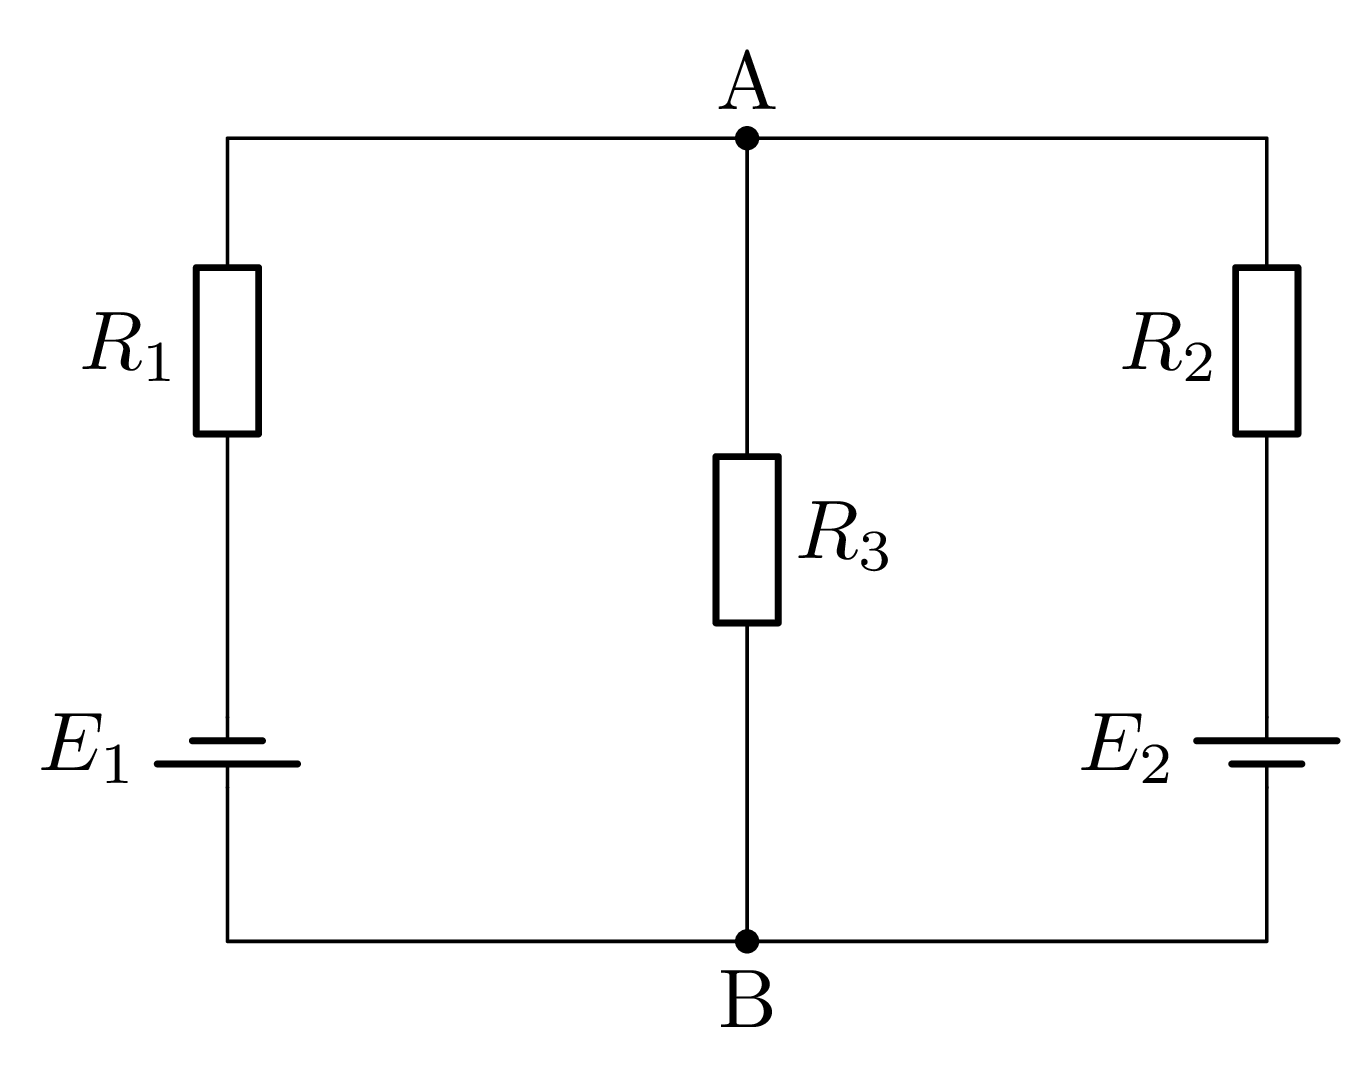
\includegraphics[keepaspectratio,width=50mm]{fig/n27_ex16_zu.png}
\end{zuright}
\end{reidai}

\begin{sisinE}
(1) 点$\mathrm{A}$には，左の枝から$I_1$，右の枝から$I_2$が流れ込む（上向きが正なので）．第一法則より，$R_3$には下向きに$I_1+I_2$が流れる．
こうしておけば未知数は$I_1$，$I_2$の2つで済む．

(2) 未知数が2つなので，独立な閉ループの式を2本立てる．左のループ（$E_1\to R_1\to\mathrm{A}\to R_3\to\mathrm{B}$）と右のループ（$E_2\to R_2\to\mathrm{A}\to R_3\to\mathrm{B}$）を選ぶとよい．
\end{sisinE}

\Key{第一法則：流入量$=$流出量\quad 第二法則：$\sum E=\sum RI$\quad 消費電力$P=RI^2$}

\begin{kaitou}
\begin{komon}
\ko{1} 点$\mathrm{A}$に流れ込む電流は$I_1+I_2$であり，これがすべて$R_3$を通って出ていくので，
       \[R_3\ \text{には下向きに}\ I_1+I_2\U{A}\Ans\]
\ko{2} 左のループ，右のループについて第二法則を立てると
       \Ana{8.0=4.0I_1+5.0(I_1+I_2),\qquad 13=10I_2+5.0(I_1+I_2)\Ans}
\ko{3} 整理すると$9I_1+5I_2=8$，$5I_1+15I_2=13$．これを解いて
       \[I_1=0.50\U{A},\qquad I_2=0.70\U{A}\]
       よって，$R_1$：上向きに$0.50\U{A}$，$R_2$：上向きに$0.70\U{A}$，$R_3$：下向きに$1.2\U{A}$\Ans
\ko{4} $P=RI^2$より
       \[P_1=4.0\times 0.50^2=1.0\U{W},\quad P_2=10\times 0.70^2=4.9\U{W},\quad P_3=5.0\times 1.2^2=7.2\U{W}\Ans\]
       \begin{chuu}
       2つの電池がする仕事率は$E_1I_1+E_2I_2=4.0+9.1=13.1\U{W}$で，消費電力の合計$1.0+4.9+7.2=13.1\U{W}$と一致する（エネルギー保存）．検算に使える．
       \end{chuu}
\end{komon}
\end{kaitou}
\end{reidaiunit}

\subsection{ホイートストンブリッジ・メートルブリッジ・ポテンシオメータ}

\begin{zuright}{44mm}
\hspace{1zw}未知抵抗の抵抗値を精密に測定するためには，次に述べるホイートストンブリッジや，これを応用したメートルブリッジが用いられる．
ホイートストンブリッジは，抵抗値$R_1$，$R_2$，$R_3$，$R_4\U{\Omega}$の4つの抵抗を，検流計$\mathrm{G}$（微弱な電流を検出する電流計），電池$E$とともに図のように接続した回路である．
第26回の26.9で見たように，{\gtfamily 検流計$\mathrm{G}$に電流が流れない場合は，}
\zusep

\includegraphics[keepaspectratio,width=44mm]{text2_p55_fig1.png}
\end{zuright}
\AnaBD{R_1:R_2=R_3:R_4}
の関係が成立する．
$R_1$，$R_2$，$R_3$の値が分かっていて，$\mathrm{G}$の電流が$0$になるように調節できれば，$R_4$が求められる．
{\gtfamily 電流が流れないことを確かめて測る}ので，検流計の内部抵抗の影響を受けず，精密に測定できる．

% 加筆：メートルブリッジ（練習［71］）とポテンシオメータ（練習［73］）の原理．
{\gtfamily メートルブリッジ}は，ホイートストンブリッジの2つの抵抗のかわりに，一様な太さの抵抗線$\mathrm{AB}$と，その上をすべる接点$\mathrm{C}$を用いたものである．
抵抗線の抵抗は長さに比例するので，{\gtfamily $\mathrm{AC}$部分と$\mathrm{CB}$部分をそれぞれ1つの抵抗とみなせば}ホイートストンブリッジそのものになり，長さの比が抵抗値の比になる（例題17(2)）．

同じ考え方で，電池の起電力を精密に測ることもできる．
電池の端子に電圧計をつなぐと，電圧計にわずかに電流が流れるため，内部抵抗による電圧降下の分だけ小さい値を測ってしまう．
そこで，一様な抵抗線に一定の電流を流しておき，測りたい電池を検流計を通して抵抗線の一部と向かい合わせにつなぐ．
検流計に電流が流れない位置を探せば，{\gtfamily そのとき電池には電流が流れていないので，内部抵抗の影響を受けずに起電力そのものが抵抗線の電圧降下と等しくなる}．
この装置を{\gtfamily ポテンシオメータ}という（練習［73］）．

\bsNeed{30mm}
\begin{matome}{ブリッジ回路}
 \hspace{3mm} 検流計$\mathrm{G}$に電流が流れない\ $\iff$\ $\mathrm{G}$の両端が等電位\ $\iff$\ $R_1:R_2=R_3:R_4$\\
 \hspace{3mm} 一様な抵抗線は，接点で分けた2つの部分をそれぞれ長さに比例する抵抗とみなす
\end{matome}

%%%%%%%%%%  例題17（原本の【例題20】）  %%%%%%%%%%%%%%%%%%%%
\bsNeed{70mm}
\begin{reidaiunit}
\begin{reidai}{ホイートストンブリッジ・メートルブリッジ}
\begin{komon}
\ko{1} 右下図のホイートストンブリッジにおいて，検流計$\mathrm{G}$に全く電流が流れないとき，$R_1$，$R_2$，$R_3$，$R_4\U{\Omega}$の間には$R_1R_4=R_2R_3$の関係が成立する．これを証明せよ．
\end{komon}
\begin{zuright}{56mm}
\begin{komon}
\ko{2} 右図はメートルブリッジと呼ばれる抵抗測定のための回路である．$\mathrm{AB}$は一様な断面積を持つ抵抗線であり，$R_0$は抵抗値$R_0\U{\Omega}$の標準抵抗，$R$は未知抵抗である．今，検流計$\mathrm{G}$と抵抗線の接点$\mathrm{C}$を動かしていったところ，$\mathrm{AC}=l_1\U{m}$，$\mathrm{CB}=l_2\U{m}$のときに検流計$\mathrm{G}$に全く電流が流れなかった．未知抵抗の抵抗値$R\U{\Omega}$を求めよ．
\end{komon}
\zusep
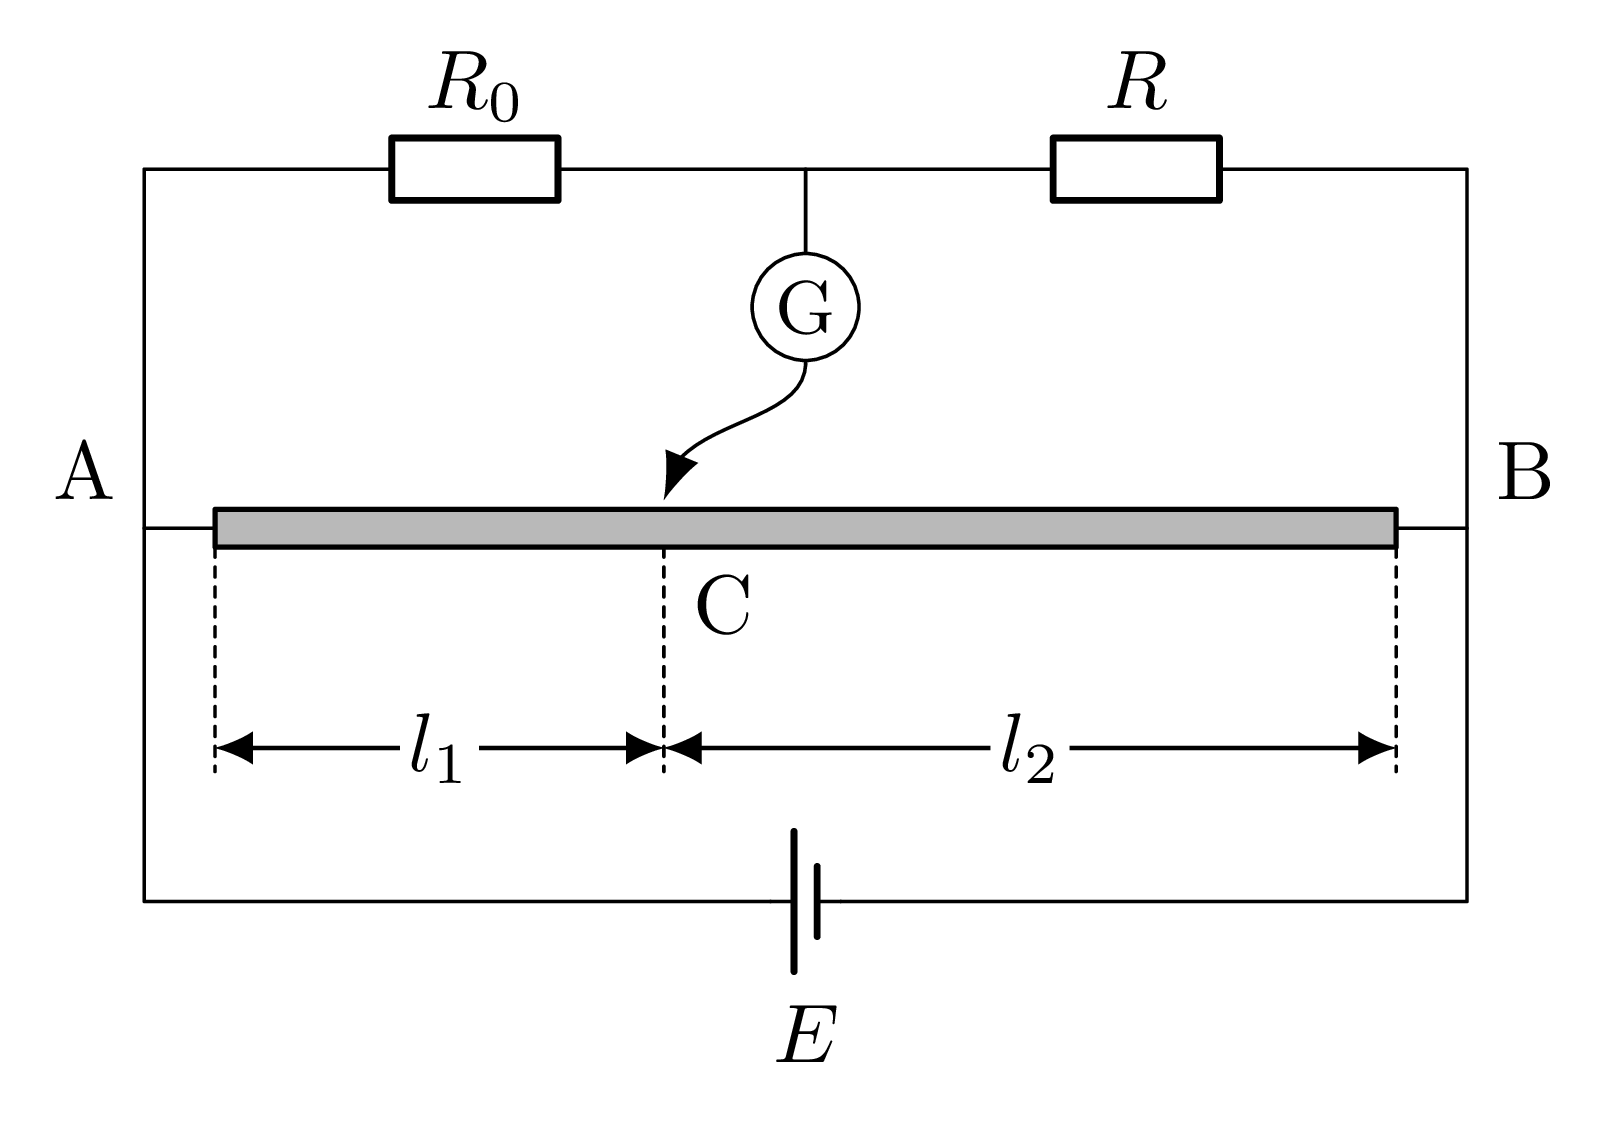
\includegraphics[keepaspectratio,width=56mm]{fig/n27_ex17_zu2.png}
\end{zuright}
\begin{center}
\includegraphics[keepaspectratio,width=36mm]{text2_p55_fig1.png}\end{center}
\end{reidai}

\begin{sisinE}
(1) $\mathrm{G}$に電流が流れないということは，$\mathrm{G}$の両端$\mathrm{B}$，$\mathrm{C}$が等電位だということである．
また，$\mathrm{G}$に電流が流れないので，$R_1$と$R_3$，$R_2$と$R_4$にはそれぞれ同じ電流が流れる．
この2つを式にすればよい．

(2) 抵抗線の$\mathrm{AC}$部分，$\mathrm{CB}$部分をそれぞれ1つの抵抗とみなして回路を書き直すと，(1)のホイートストンブリッジになる．
抵抗線の抵抗は長さに比例する．
\end{sisinE}

\Key{ホイートストンブリッジ：$\mathrm{G}$に電流が流れない\ $\iff$\ $R_1R_4=R_2R_3$}

\begin{kaitou}
\begin{komon}
\ko{1} $\mathrm{G}$に電流が流れないので，$R_1$，$R_3$を流れる電流は等しく（$I_1$とおく），$R_2$，$R_4$を流れる電流も等しい（$I_2$とおく）．
       また$\mathrm{B}$，$\mathrm{C}$は等電位であるから，$\mathrm{A}$からの電圧降下どうし，$\mathrm{D}$までの電圧降下どうしが等しい：
       \Ana{R_1I_1=R_2I_2,\qquad R_3I_1=R_4I_2}
       辺々割ると$\dfrac{R_1}{R_3}=\dfrac{R_2}{R_4}$，すなわち$R_1R_4=R_2R_3$が成り立つ．\Ans
\ko{2} 抵抗線の抵抗率を$\rho$，断面積を$S$とすると，$\mathrm{AC}$部分，$\mathrm{CB}$部分の抵抗は$R_{\mathrm{AC}}=\rho\dfrac{l_1}{S}$，$R_{\mathrm{CB}}=\rho\dfrac{l_2}{S}$である．
       回路はホイートストンブリッジと同じなので，(1)より$R_0:R_{\mathrm{AC}}=R:R_{\mathrm{CB}}$．よって
       \[R=\frac{R_{\mathrm{CB}}}{R_{\mathrm{AC}}}R_0=\frac{l_2}{l_1}R_0\U{\Omega}\Ans\]
       （$\rho$と$S$は消えるので，長さの比だけを測ればよい．）
\end{komon}
\end{kaitou}
\end{reidaiunit}

\subsection{コンデンサーの過渡現象}

抵抗とコンデンサーを組み合わせた回路では，電流の流入によってコンデンサーの極板に電荷がたまり，極板間に電位差が生じる．
極板に電荷がたまっていく途中の様子を詳しく知るのは難しいが，{\gtfamily 十分に時間が経過するとコンデンサーの極板上の電荷は一定値となり，コンデンサーには電流が流れ込まなくなる}．
このように，見かけ上，回路に変化が起こらなくなった状態を{\gtfamily 定常状態}と呼ぶ．
定常状態で流れる電流や蓄えられている電荷は容易に求めることができる．
変化の途中の状態を{\gtfamily 過渡状態}，その現象を{\gtfamily 過渡現象}という．

抵抗とコンデンサーを含む回路の問題では，次の2点を押さえておくことが重要である．
\begin{description}
\item[\MARU{1}] {\gtfamily スイッチ操作の直前と直後で，コンデンサーに蓄えられている電荷は等しい}（電荷が移動するには時間がかかるから）．
      したがって，電荷が$0$のコンデンサーはスイッチを入れた直後は{\gtfamily ただの導線}とみなせる（電位差$\dfrac{Q}{C}=0$）．
\item[\MARU{2}] {\gtfamily 十分時間が経過すると，コンデンサーの電荷は一定となり，コンデンサーには電流が流れない}（コンデンサーの枝は切れているのと同じ）．
\end{description}

% 加筆：電池の仕事と静電エネルギーの差（第25回の 25.2 で予告．例題18(6)・練習［74］）．
電池がコンデンサーを充電するとき，電池は電荷$Q$を電位差$V$だけ持ち上げるので$W=QV$の仕事をするが，コンデンサーに蓄えられる静電エネルギーは$U=\dfrac{1}{2}QV$である（25.2）．
その差$\dfrac{1}{2}QV$は，充電の途中で電流が流れた{\gtfamily 抵抗でジュール熱として失われる}．
この値は抵抗値によらない（抵抗が小さいと大きな電流が短い時間流れ，大きいと小さな電流が長い時間流れる）．

\bsNeed{34mm}
\begin{matome}{コンデンサーを含む回路}
 \hspace{3mm} スイッチ操作の直前直後：\AnaB{コンデンサーの電荷は変わらない}\\
 \hspace{3mm} 十分時間が経過した後：\AnaB{コンデンサーには電流が流れない}\\
 \hspace{3mm} 充電の間：電池の仕事$QV$＝静電エネルギー$\dfrac{1}{2}QV$＋ジュール熱$\dfrac{1}{2}QV$
\end{matome}

%%%%%%%%%%  例題18（原本の【例題21】）  %%%%%%%%%%%%%%%%%%%%
\bsNeed{60mm}
\begin{reidaiunit}
\begin{reidai}{コンデンサーの過渡現象}
\begin{zuright}{40mm}
\hspace{1zw}右図のように抵抗値$R\U{\Omega}$の抵抗，電気容量$C\U{F}$のコンデンサー，起電力$V\U{V}$の電池とスイッチ$\mathrm{S}$からなる回路をつくる．はじめスイッチ$\mathrm{S}$は開いており，コンデンサーの極板には電荷は蓄えられていないものとする．スイッチを閉じてコンデンサーが充電される間について，以下の問いに答えよ．
\zusep
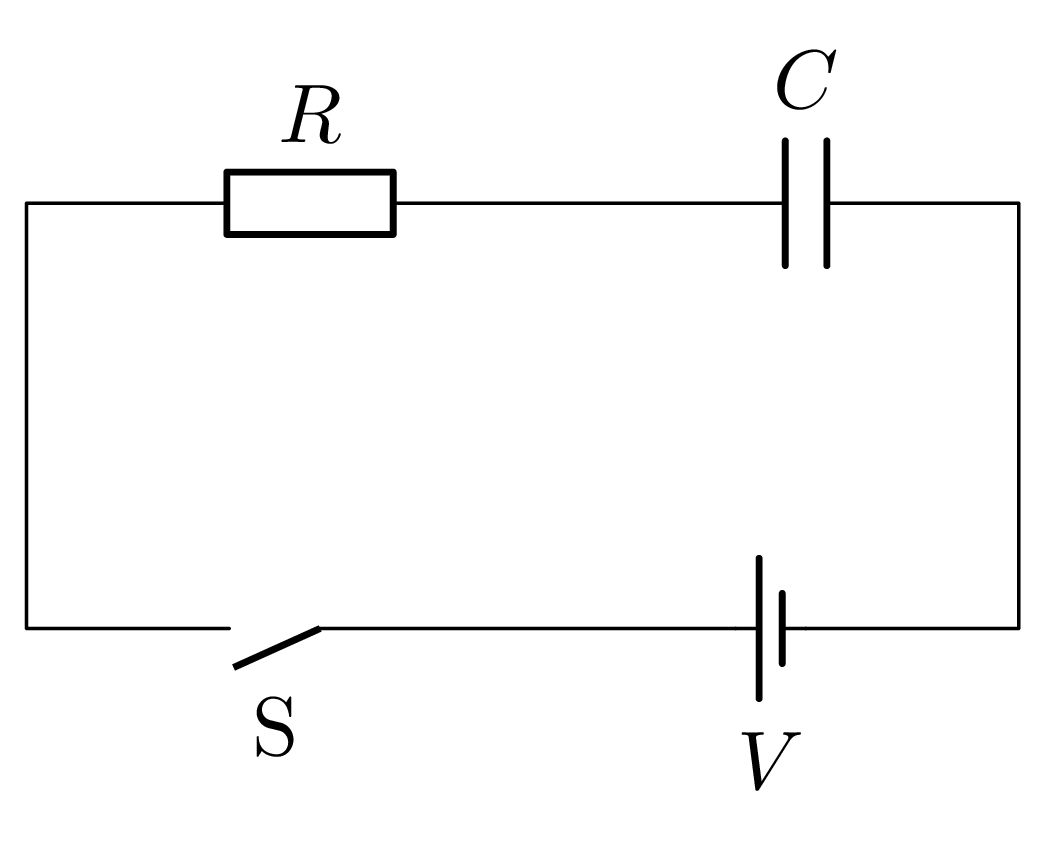
\includegraphics[keepaspectratio,width=36mm]{fig/n27_ex18_zu.png}
\end{zuright}
\begin{komon}
\ko{1} コンデンサーの左側極板に蓄えられる電荷を$Q\U{C}$，抵抗を図の向きに流れる電流を$I\U{A}$とする．この回路において成立するキルヒホッフの第二法則を記せ．
\ko{2} コンデンサーの極板に流れ込む電流に注目して，$I$と$Q$の間に成立する関係式を，微分を用いて示せ．
\ko{3} スイッチを閉じた直後，コンデンサーに蓄えられている電荷は$0\U{C}$のままである．スイッチを閉じた直後に抵抗を流れる電流$I_0\U{A}$を求めよ．
\ko{4} スイッチを閉じると，徐々にコンデンサーに電荷が蓄えられていき，ある一定値に近づいていく．十分時間が経過したときのコンデンサーに蓄えられる電荷$Q_\infty\U{C}$を求めよ．
\ko{5} (3)(4)を元に，スイッチを閉じた後の$Q$の時間変化を表すグラフの形を描け．
\ko{6} スイッチを閉じてから十分時間が経過する間に，電池がした仕事$W\U{J}$，コンデンサーに蓄えられた静電エネルギー$\varDelta U\U{J}$，抵抗で消費されたジュール熱$J\U{J}$を求めよ．
\end{komon}
\end{reidai}

\begin{sisinE}
(1)(2) 電流$I$が流れ込むと極板の電荷$Q$が増える．単位時間あたりに流れ込む電気量が電流なので，$Q$の増加率$\dfrac{dQ}{dt}$が$I$である．

(3)(4) 過渡現象の2つのポイント（直後はコンデンサーの電荷が$0$のまま／十分時間後は電流が$0$）を(1)の式に当てはめる．

(5) $Q$は$0$から始まり，$CV$に近づく．$Q$-$t$グラフの傾きは$\dfrac{dQ}{dt}=I$であり，$I$は(1)の式から$Q$が増えるほど小さくなる．
\end{sisinE}

\Key{スイッチ操作直後：コンデンサーの電荷は変わらない\quad 十分時間後：コンデンサーに電流は流れない\quad $I=\dfrac{dQ}{dt}$}

\begin{kaitou}
\begin{komon}
\ko{1} 抵抗で$RI$，コンデンサーで$\dfrac{Q}{C}$だけ電位が下がるので，
       \Ana{V=RI+\frac{Q}{C}\Ans}
\ko{2} 極板に流れ込む電流が極板の電荷を増やすので，
       \[I=\frac{dQ}{dt}\Ans\]
\ko{3} $Q=0$を(1)に代入して，
       \[I_0=\frac{V}{R}\U{A}\Ans\]
\ko{4} 十分時間が経つと$I=0$になるので，(1)より
       \[Q_\infty=CV\U{C}\Ans\]
\ko{5} $Q$は$0$から増加し，$CV$に漸近する．グラフの傾き$\dfrac{dQ}{dt}=I$は，はじめ$\dfrac{V}{R}$で，(1)より$Q$が増えるほど小さくなっていく．よって次図のようになる．\Ans
       \begin{center}\AnaFig{58mm}{fig/n27_ex18_ans.png}{fig/n27_ex18_ans_blank.png}\end{center}
\ko{6} この間に電池を通過した電気量は$CV$なので，電池のした仕事は
       \[W=CV\cdot V=CV^2\U{J}\Ans\]
       \[\varDelta U=\frac{1}{2}CV^2\U{J}\Ans\]
       エネルギー保存より
       \Ana{J=W-\varDelta U=\frac{1}{2}CV^2\U{J}\Ans}
       \begin{bsHosoku}{参考}
       (1)(2)より$V=R\dfrac{dQ}{dt}+\dfrac{Q}{C}$という微分方程式が得られ，これを解くと$Q=CV\bigl(1-e^{-\frac{t}{RC}}\bigr)$となる．$RC$（単位は$\U{s}$）を{\gtfamily 時定数}といい，充電の速さの目安である．$t=RC$で$Q$は最終値の約$63\,\%$に達する．なお，$J=\displaystyle\int_0^\infty RI^2\,dt$を実際に計算しても$\dfrac{1}{2}CV^2$になる．
       \end{bsHosoku}
\end{komon}
\end{kaitou}
\end{reidaiunit}

\subsection{抵抗・コンデンサーの複合回路}

過渡現象の2つのポイントに注意して，コンデンサーと抵抗を含む回路を解いてみよう．
定常状態ではコンデンサーの枝に電流が流れないので，{\gtfamily 電流の分布は，コンデンサーの枝を取り除いた回路と同じになる}．
まずその回路で電流を求め，次にコンデンサーを含む閉ループに第二法則を使ってコンデンサーの電圧（電荷）を求める，という順に進めるとよい．
浮いている部分があれば，第25回と同じく電荷保存の法則も使う．

%%%%%%%%%%  例題19（原本の【例題22】）  %%%%%%%%%%%%%%%%%%%%
\bsNeed{60mm}
\begin{reidaiunit}
\begin{reidai}{抵抗・コンデンサー複合回路}
\begin{zuright}{58mm}
\hspace{1zw}図のように，抵抗値がそれぞれ$R$，$R$，$2R$，$2R\U{\Omega}$の電気抵抗$R_1$，$R_2$，$R_3$，$R_4$，電気容量がそれぞれ$2C$，$C\U{F}$のコンデンサー$C_1$，$C_2$，およびスイッチ$\mathrm{S}_1$，$\mathrm{S}_2$，内部抵抗の無視できる起電力$V\U{V}$の電池$E$を用いて図のような回路を作り，$\mathrm{A}$点を接地する．最初，スイッチはいずれも開いており，コンデンサーの極板上には電荷はなかった．$\mathrm{A}$点の電位を$0\U{V}$として，以下の設問に答えよ．
\zusep
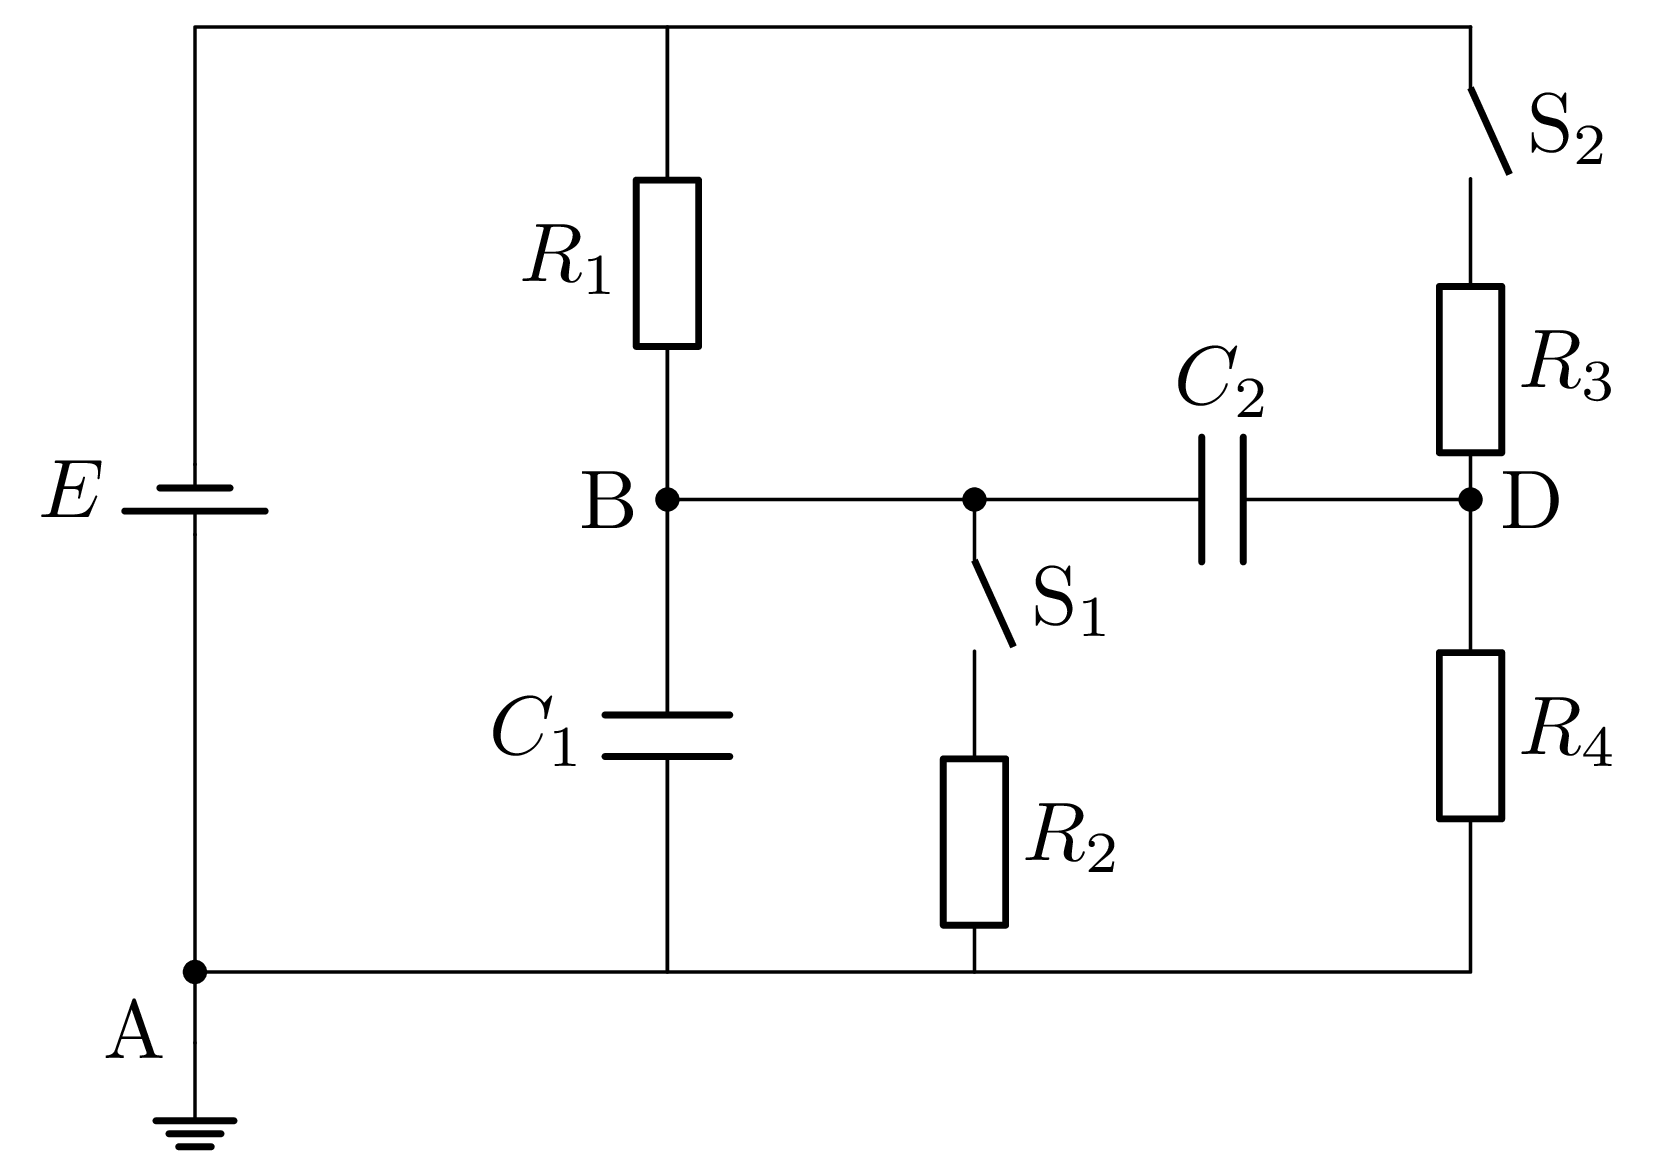
\includegraphics[keepaspectratio,width=58mm]{fig/n27_ex19_zu.png}
\end{zuright}
\begin{komon}
\ko{1} スイッチ$\mathrm{S}_1$，$\mathrm{S}_2$を開いたままで十分時間が経過したとき，点$\mathrm{B}$の電位を求めよ．
\ko{2} 次に，スイッチ$\mathrm{S}_1$，$\mathrm{S}_2$を閉じ，十分時間が経過したとき，抵抗$R_1$に流れている電流を求めよ．
\ko{3} (2)のとき，コンデンサー$C_1$に蓄えられている電荷を求めよ．
\ko{4} 次に，スイッチ$\mathrm{S}_1$は閉じたままでスイッチ$\mathrm{S}_2$を開いた．十分時間がたったとき，コンデンサー$C_2$に蓄えられる電荷を求めよ．
\end{komon}
\end{reidai}

\begin{sisinE}
定常状態ではコンデンサーに電流が流れ込まない．まず{\gtfamily 定常状態における電流分布がどのようになっているのか}を考えよ．
電流が流れていない抵抗では電圧降下が$0$なので，その両端は等電位である．
各点の電位が分かれば，コンデンサーの電圧は両極板の電位差として求まる．
\end{sisinE}

\Key{定常状態\ $\iff$\ コンデンサーに電流が流れ込まない\quad 電流の流れない抵抗の両端は等電位}

\begin{kaitou}
\begin{komon}
\ko{1} $\mathrm{S}_1$，$\mathrm{S}_2$が開いていると，電流の通り道は$R_1\to C_1$と$R_1\to C_2\to R_4$だけで，どちらもコンデンサーを含む．十分時間が経つとコンデンサーに電流は流れ込まないので，$R_1$にも電流が流れない．$R_1$で電圧降下が無いので，$\mathrm{B}$の電位は電池の正極と同じで
       \[V_{\mathrm{B}}=V\U{V}\Ans\]
\ko{2} 十分時間が経つとコンデンサーに電流は流れないので，電流は$R_1\to\mathrm{S}_1\to R_2$と$\mathrm{S}_2\to R_3\to R_4$の2本の道だけを流れる．$R_1$と$R_2$は直列なので
       \Ana{I_1=\frac{V}{R+R}=\frac{V}{2R}\U{A}\Ans}
\ko{3} $\mathrm{B}$の電位は$R_2$の電圧降下に等しく$V_{\mathrm{B}}=R\cdot\dfrac{V}{2R}=\dfrac{V}{2}$．$C_1$の下側極板は$\mathrm{A}$（電位$0$）につながっているので，$C_1$の電圧は$\dfrac{V}{2}$で，
       \[Q_1=2C\cdot\frac{V}{2}=CV\U{C}\Ans\]
       （$\mathrm{B}$側の極板が$+CV$．）
       \begin{chuu}
       このとき$R_3$，$R_4$にも$\dfrac{V}{4R}$が流れ，$\mathrm{D}$の電位は$2R\cdot\dfrac{V}{4R}=\dfrac{V}{2}$である．$\mathrm{B}$と$\mathrm{D}$が等電位なので，$C_2$の電荷は$0$になっている．
       \end{chuu}
\ko{4} $\mathrm{S}_2$を開くと$R_3$には電流が流れなくなり，十分時間後には$C_2$にも電流が流れないので，$R_4$にも電流が流れない．よって$\mathrm{D}$の電位は$\mathrm{A}$と同じ$0$になる．一方$R_1$，$R_2$の電流は(2)と同じなので$V_{\mathrm{B}}=\dfrac{V}{2}$のままである．$C_2$の電圧は$V_{\mathrm{B}}-V_{\mathrm{D}}=\dfrac{V}{2}$なので，
       \Ana{Q_2=C\cdot\frac{V}{2}=\frac{1}{2}CV\U{C}\Ans}
       （$\mathrm{B}$側の極板が$+\dfrac{1}{2}CV$．）
\end{komon}
\end{kaitou}
\end{reidaiunit}

\subsection{非オーム抵抗を含む回路}

第26回の26.4で見たように，電球のフィラメントなどでは電流によって温度が上がり抵抗値が変わるので，$I$-$V$特性曲線が直線にならない（非オーム抵抗）．
非オーム抵抗では$V=RI$の$R$が一定ではないので，$R$を使った計算ができない．
そこで，非オーム抵抗を含む回路に流れる電流は，次のようにして求める．

\bsNeed{40mm}
\begin{matome}{非オーム抵抗を含む回路}
 \MARU{1}\ 非オーム抵抗を流れる電流とかかる電圧を，ともに未知数として$I\U{A}$，$V\U{V}$とおく\\
 \MARU{2}\ キルヒホッフの法則の式を立てて連立し，\AnaB{$I$と$V$だけを含む関係式}を求める\\
 \MARU{3}\ 与えられた$I$-$V$特性曲線に\MARU{2}の関係式（直線になることが多い）を書き込み，\AnaB{その交点を読む}
\end{matome}

\MARU{2}の直線は，電池と抵抗の側から見た「非オーム抵抗にかけられる電圧と電流の関係」であり，特性曲線は非オーム抵抗自身の性質である．両方を同時に満たす点が実際の状態である．

% 加筆：練習［78］［79］の前提．
非オーム抵抗が2個以上あるときは，{\gtfamily 同じものが並列（直列）なら電流（電圧）が等しい}ことを使って未知数を減らす．
特性の異なる2個が並列なら特性曲線を{\gtfamily 縦に足し}，直列なら{\gtfamily 横に足し}て，1つの素子の特性曲線にまとめてから交点を取るとよい（練習［78］）．
また，非オーム抵抗のその状態での抵抗値は，特性曲線上の点の$\dfrac{V}{I}$（原点とその点を結ぶ直線の傾きの逆数）である（練習［79］）．

%%%%%%%%%%  例題20（原本の【例題23】）  %%%%%%%%%%%%%%%%%%%%
\bsNeed{70mm}
\begin{reidaiunit}
\begin{reidai}{非オーム抵抗を含む回路}
\begin{zuright}{56mm}
\hspace{1zw}定常的に点灯しているときに下図のような電流-電圧特性をもつ豆電球がある．この豆電球に$15\U{\Omega}$と$30\U{\Omega}$の抵抗を右図のように接続して，$\mathrm{PQ}$間に$12\U{V}$の電圧をかけた．このとき，以下の設問に答えよ．
\begin{komon}
\ko{1} 豆電球に流れる電流を$I\U{A}$，豆電球にかかる電圧を$V\U{V}$，$15\U{\Omega}$の抵抗に流れる電流を$i\U{A}$と置く．このとき，$I$，$V$，$i$の間に成立する関係式を2つ立てよ．
\ko{2} $I$と$V$の間に成立する，$i$を含まない関係式を求めよ．
\ko{3} 豆電球に流れる電流$I\U{A}$およびかかる電圧$V\U{V}$を求めよ．
\end{komon}
\zusep
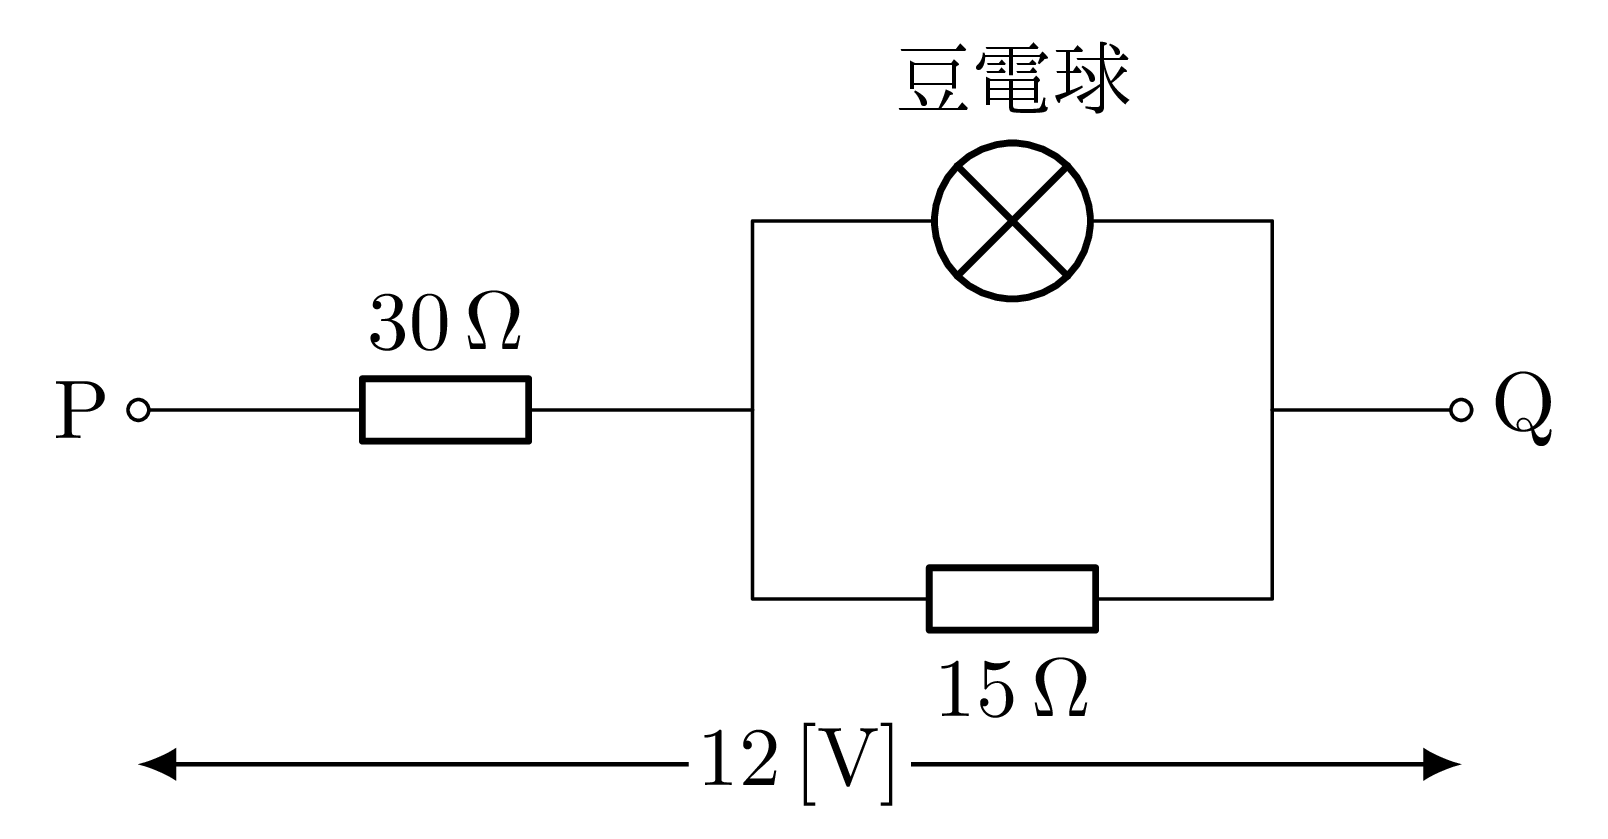
\includegraphics[keepaspectratio,width=56mm]{fig/n27_ex20_zu.png}
\end{zuright}
\begin{center}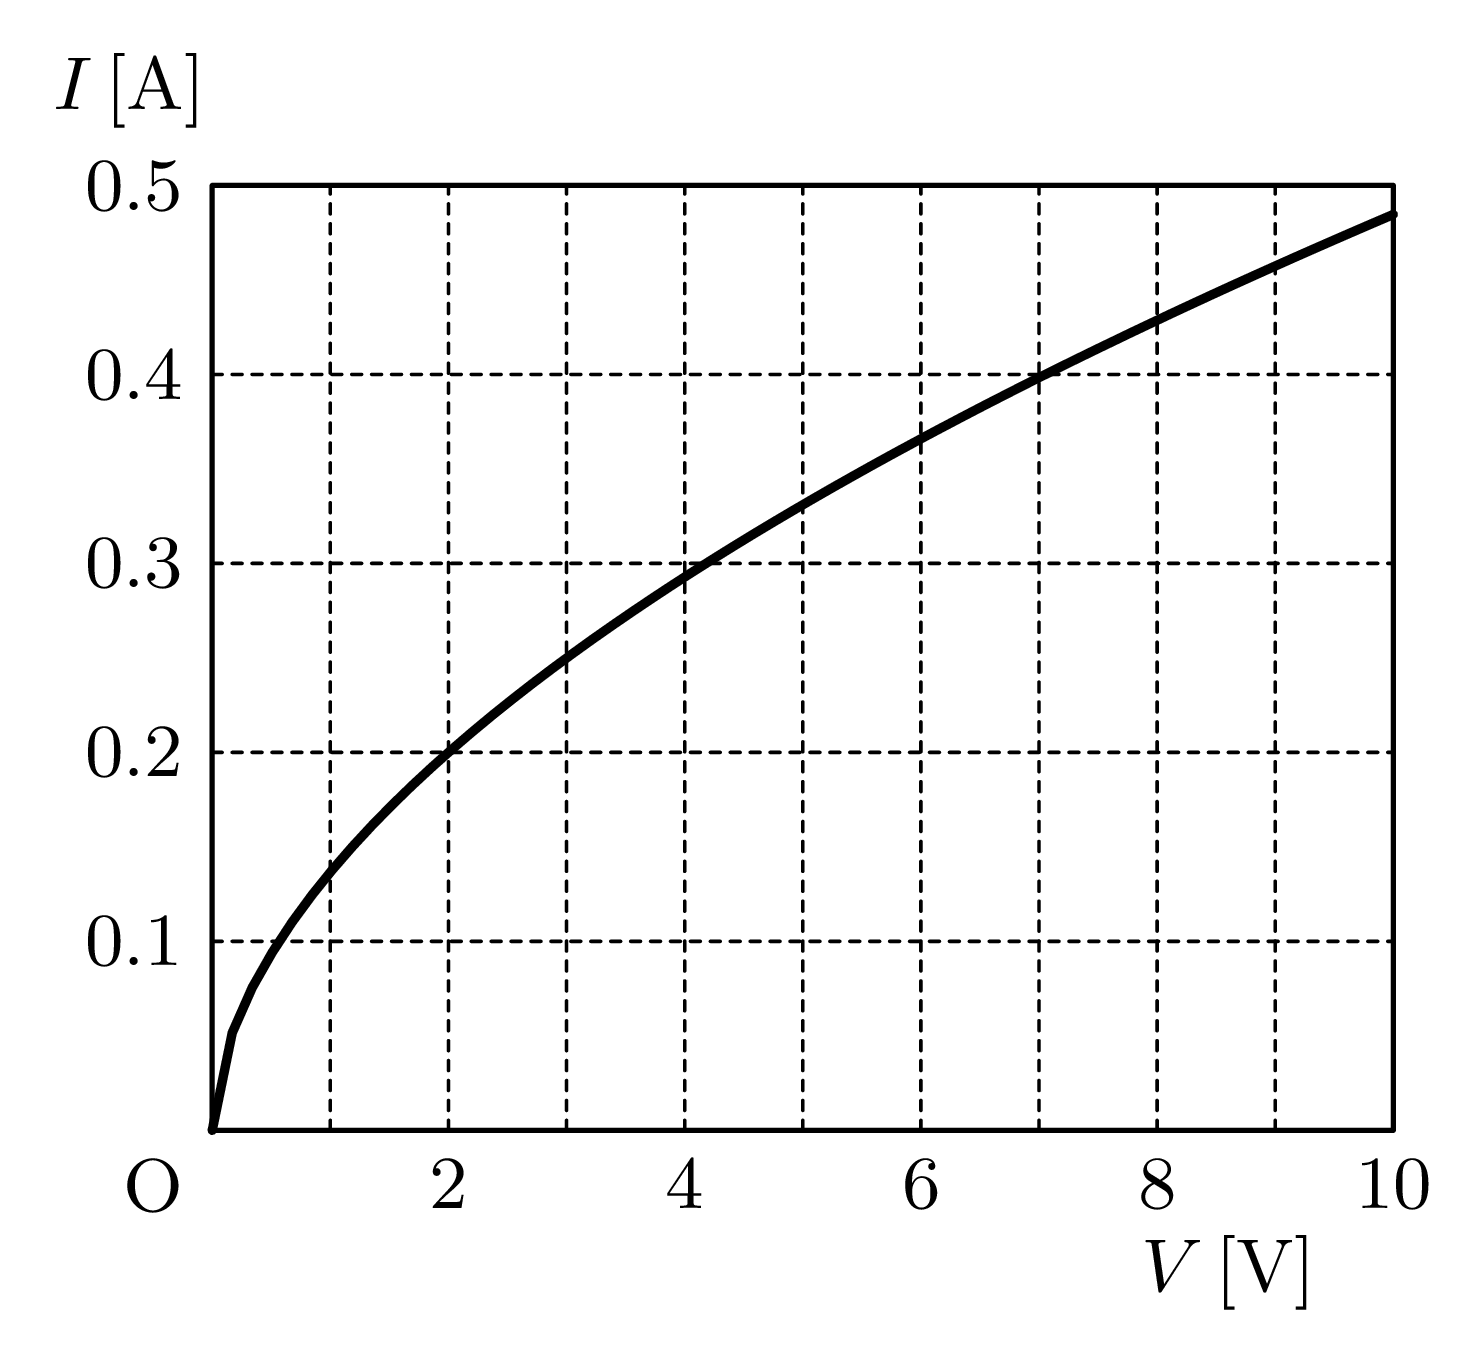
\includegraphics[keepaspectratio,width=52mm]{fig/n27_ex20_graph.png}\end{center}
\end{reidai}

\begin{sisinE}
豆電球は非オーム抵抗なので，$I$と$V$をともに未知数として置き，$V=RI$の形は使わない．
豆電球と$15\U{\Omega}$は並列なので電圧が等しい．$30\U{\Omega}$には両者の電流の和が流れる．
\end{sisinE}

\Key{非オーム抵抗を流れる電流$I\U{A}$，かかる電圧$V\U{V}$をともに未知数とし，特性曲線との交点を取る}

\begin{kaitou}
\begin{komon}
\ko{1} 豆電球と$15\U{\Omega}$の抵抗は並列なので同じ電圧$V$がかかる：$V=15i$．
       また，$30\U{\Omega}$には$I+i$が流れるので，$\mathrm{PQ}$間について第二法則より$12=30(I+i)+V$．
       \Ana{V=15i,\qquad 12=30(I+i)+V\Ans}
\ko{2} 第1式より$i=\dfrac{V}{15}$を第2式に代入して，
       \[12=30I+2V+V\qquad\therefore\ I=0.4-\frac{V}{10}\Ans\]
\ko{3} (2)の直線を特性曲線に書き込み，交点を読むと
       \begin{center}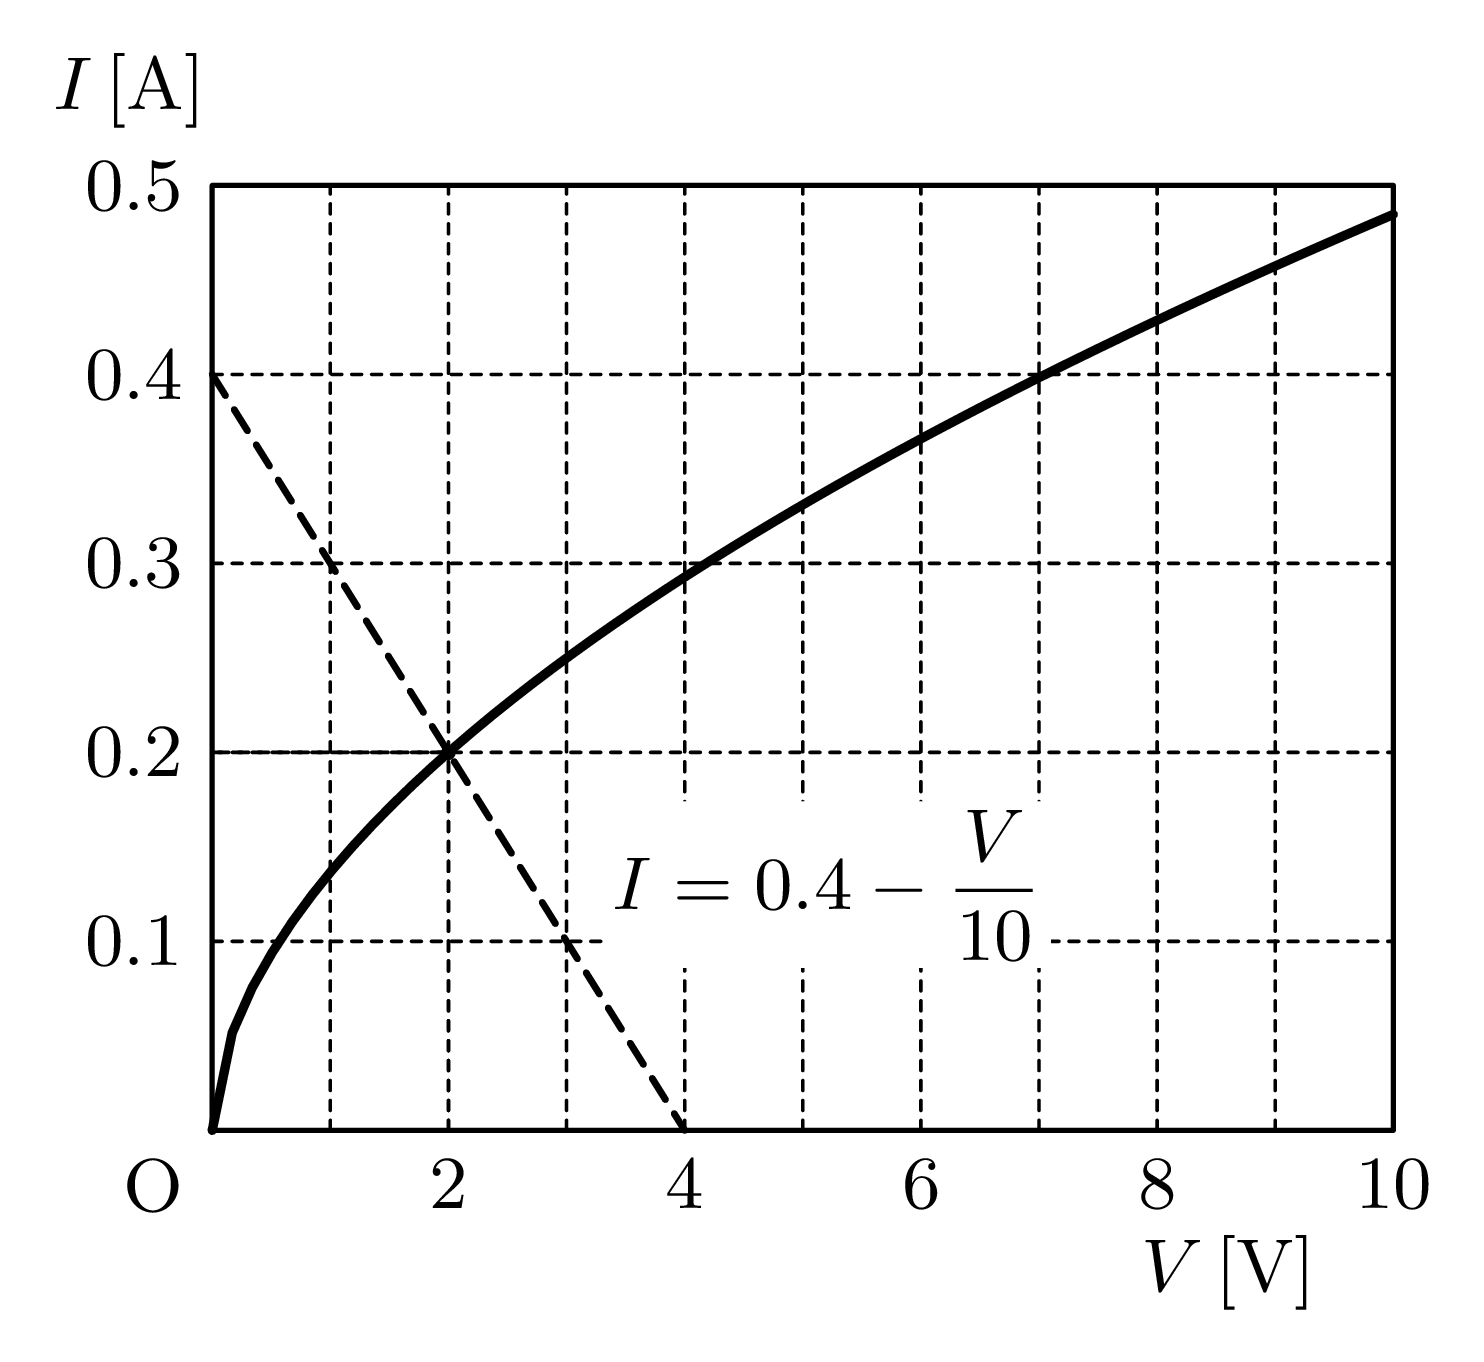
\includegraphics[keepaspectratio,width=50mm]{fig/n27_ex20_ans.png}\end{center}
       \Ana{I=0.20\U{A},\qquad V=2.0\U{V}\Ans}
\end{komon}
\end{kaitou}
\end{reidaiunit}

\subsection{ダイオード}

\begin{zuright}{64mm}
\hspace{1zw}$\mathrm{N}$型半導体と$\mathrm{P}$型半導体（第26回 26.5）を接合（$\mathrm{PN}$接合）した素子を{\gtfamily ダイオード}という．
$\mathrm{N}$型半導体は，正に帯電して動けないドナーの周りに自由電子があるので，全体としては帯電していない．
また，$\mathrm{P}$型半導体も同様に，動けないアクセプターの周りに正孔があるため，全体としては帯電していない．

\hspace{1zw}この$\mathrm{P}$型半導体と$\mathrm{N}$型半導体を接合すると，接合の境界面の前後では，拡散して（ランダムに動いて）電子と正孔がぶつかり，境界面で結合して消える（再結合）．
その結果，境界面の前後にはキャリアが存在しない領域ができる．この領域を{\gtfamily 空乏層}という．

\hspace{1zw}空乏層にはイオン化したドナー，アクセプターが残り，その電荷の偏りによって$\mathrm{N}$型から$\mathrm{P}$型の向きに電場が発生する．
空乏層ができた後に電子と正孔が再結合するためには，この電場に逆らって移動しなければならない．
その結果，空乏層にはほとんどキャリアが存在しなくなる．
\zusep

\includegraphics[keepaspectratio,width=64mm]{text2_p59_fig1.png}
\end{zuright}

$\mathrm{P}$の方が高電位になるように電圧をかける（{\gtfamily 順方向}）と，空乏層の電場が弱められ，電子と正孔は空乏層に入り込みやすくなる（空乏層が狭くなる）ので，$\mathrm{P}$型$\to\mathrm{N}$型の向きに電流が流れやすくなる．
ただし，かける電圧が小さいうちは電流はほとんど流れない．
一方，逆向きに電圧をかける（{\gtfamily 逆方向}）と空乏層内の電場がさらに強くなり，空乏層は広がり，電子と正孔は境界面に近づけなくなるので，電流は流れない．
このように，{\gtfamily ダイオードは順方向にのみ電流を流す}．これを{\gtfamily 整流作用}という．

\begin{center}

\includegraphics[keepaspectratio,width=112mm]{text2_p59_fig2.png}
\end{center}

{\gtfamily 発光ダイオード}（LED）は，接合面付近で電子と正孔が再結合する際に生じるエネルギーを光として放出する．
逆に，$\mathrm{PN}$接合面付近に光が入射すると，そのエネルギーで自由電子と正孔が生じ，空乏層の電場によって互いに逆向きに移動するので，ダイオードの逆方向に電流を流すことができる．
この仕組みを利用して{\gtfamily 太陽電池}は発電を行っている．

回路の問題では，ダイオードは{\gtfamily $I$-$V$特性曲線が与えられた非オーム抵抗}として，27.5 と同じ方法で扱えばよい（練習［80］）．

\bsNeed{26mm}
\begin{matome}{ダイオード}
 \hspace{3mm} $\mathrm{P}$型と$\mathrm{N}$型の接合．\AnaB{$\mathrm{P}\to\mathrm{N}$の向き}（順方向）にだけ電流を流す（整流作用）\\
 \hspace{3mm} 回路の中では，特性曲線をもつ非オーム抵抗として扱う
\end{matome}

\newpage

%%%%%%%%%%%%%%%%%%%%  練習問題  %%%%%%%%%%%%%%%%%%%%
% 第26回の［68］に続く．
\setcounter{qno}{68}

\filbreak
\Rank{A問題}

\Mon{基本公式の確認}

\begin{zuright}{50mm}
\hspace{1zw}以下の設問に答えよ．
\begin{komon}
\ko{1} 内部抵抗が$10\U{\Omega}$で，最大$5\U{mA}$まで測定可能な電流計がある．この電流計を使って最大$1\U{A}$まで測定可能な電流計にするためには何$\U{\Omega}$の抵抗を並列に接続すればよいか．
\ko{2} 内部抵抗が$1\U{k\Omega}$で，最大$1\U{V}$まで測定可能な電圧計がある．この電圧計を使って最大$100\U{V}$まで測定可能な電圧計にするためには何$\U{\Omega}$の抵抗を直列に接続すればよいか．
\ko{3} 両端にかかる電圧の値と流れる電流の値の関係が右図で示される電球に$100\U{V}$の電池と$100\U{\Omega}$の抵抗を直列に接続した．このとき電球を流れる電流の強さは何$\U{A}$か．
\end{komon}
\zusep
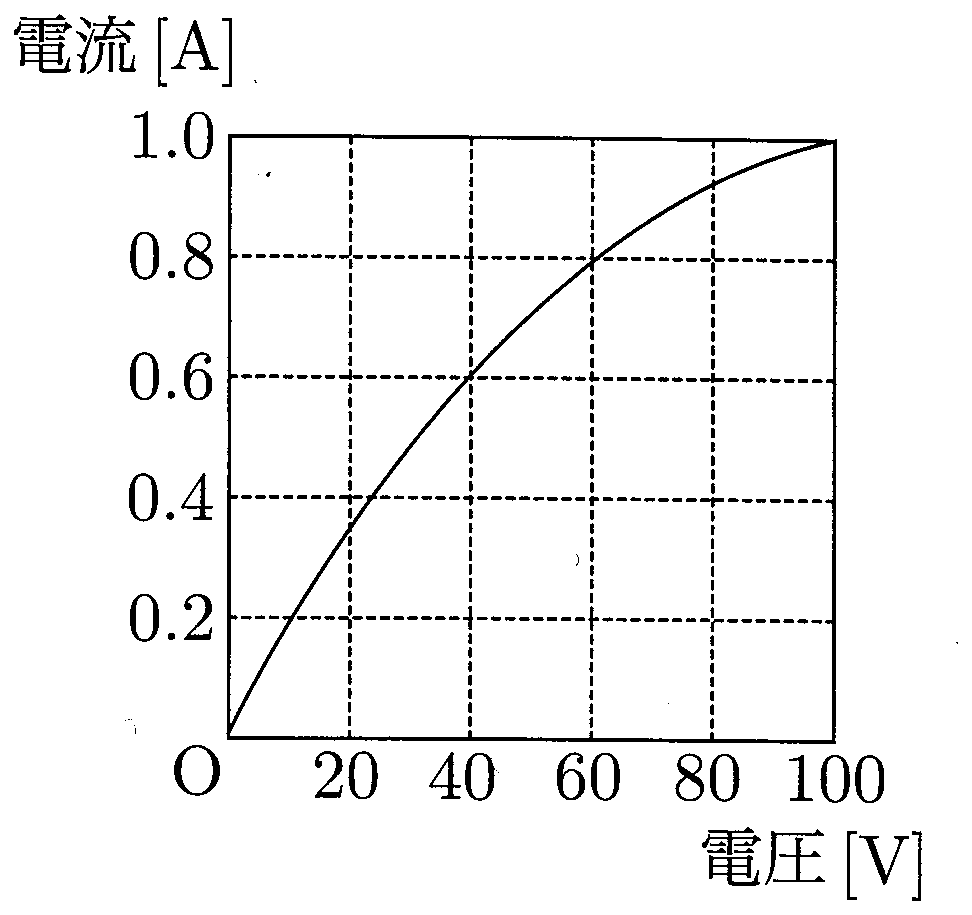
\includegraphics[keepaspectratio,width=44mm]{fig/n27_p69_graph.png}\\[2mm]
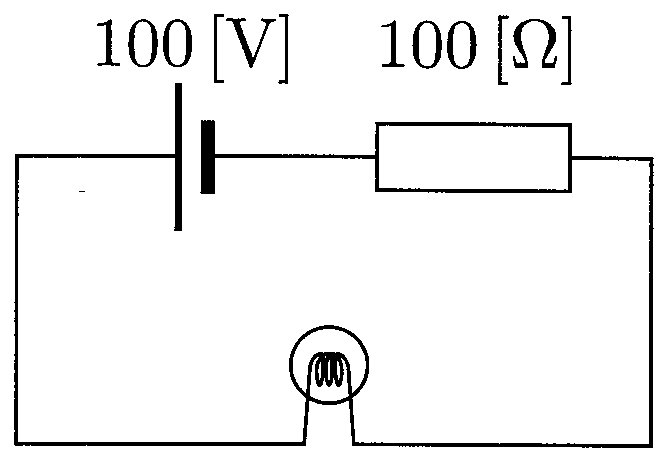
\includegraphics[keepaspectratio,width=40mm]{fig/n27_p69_zu.png}
\end{zuright}

\filbreak
\Rank{B問題}

\Mon{キルヒホッフの法則の適用}

\begin{zuright}{46mm}
\hspace{1zw}内部抵抗の無視できる起電力$20$，$10\U{V}$の電池$\mathrm{E}_1$，$\mathrm{E}_2$と，抵抗値$15$，$10$，$5.0\U{\Omega}$の抵抗$\mathrm{R}_1$，$\mathrm{R}_2$，$\mathrm{R}_3$を右図のように接続した．これについて以下の設問に答えよ．
\begin{komon}
\ko{1} $\mathrm{R}_1$，$\mathrm{R}_2$の抵抗を左向きに流れる電流の強さをそれぞれ$I_1$，$I_2\U{A}$とおく．このとき，$\mathrm{R}_3$の抵抗に流れる電流の向きとその強さを求めよ．
\ko{2} キルヒホッフの第二法則を用いて成立する式を示せ．
\ko{3} 各抵抗に流れる電流の向きとその強さを求めよ．
\end{komon}
\zusep
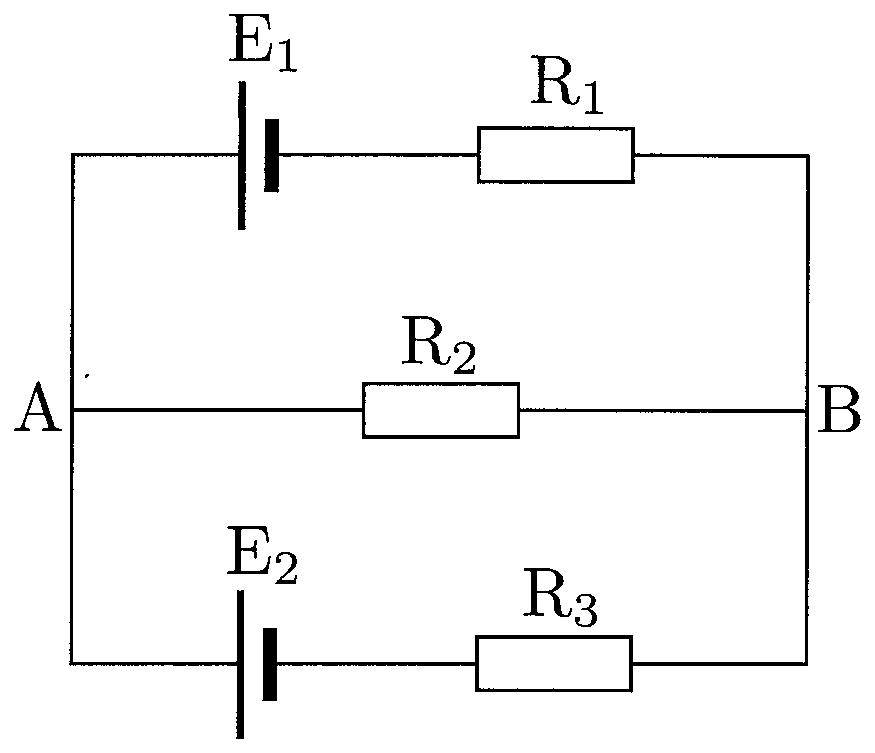
\includegraphics[keepaspectratio,width=44mm]{fig/n27_p70_zu.png}
\end{zuright}

\Mon{メートルブリッジ}

\begin{zuright}{50mm}
\hspace{1zw}右図はメートルブリッジと呼ばれる抵抗値測定のための回路である．$\mathrm{E}$は電池，$\mathrm{AB}$は長さ$l_0\U{m}$の一様な太さの抵抗線，$\mathrm{R}_0$は抵抗値$R_0\U{\Omega}$の標準抵抗，そして$\mathrm{R}$は未知抵抗である．今，検流計$\mathrm{G}$と抵抗線$\mathrm{AB}$の接触点$\mathrm{P}$を動かしていき$\mathrm{AP}=x\U{m}$となったとき，検流計$\mathrm{G}$には電流が流れなくなった．このことを用いて，この未知抵抗$\mathrm{R}$の抵抗値を求めよ．
\zusep
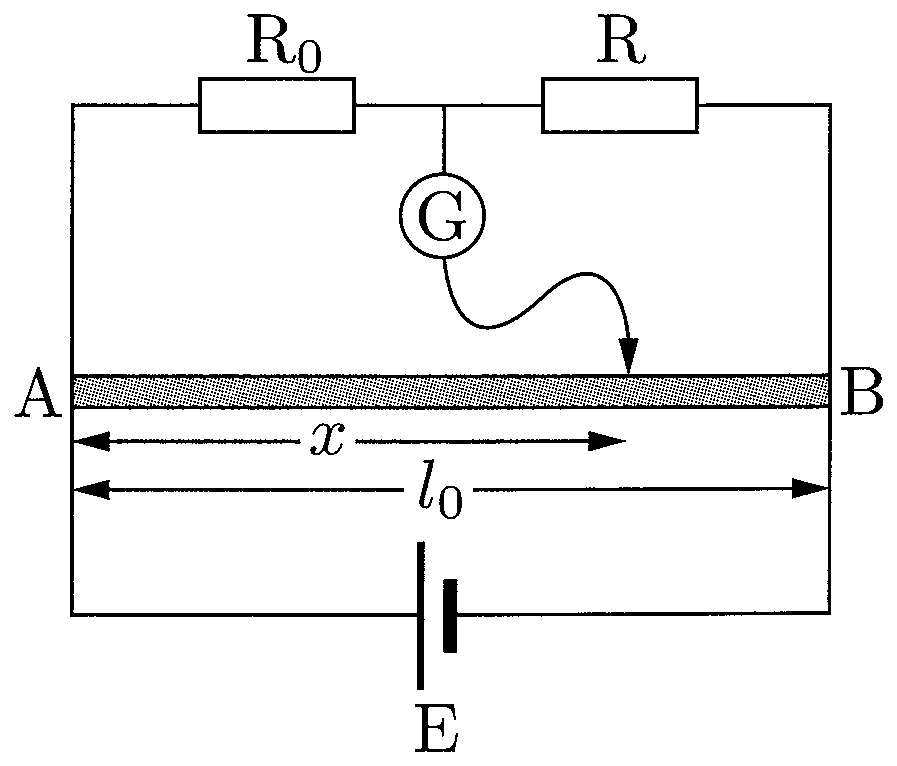
\includegraphics[keepaspectratio,width=46mm]{fig/n27_p71_zu.png}
\end{zuright}

\Mon[\Sitei]{可変抵抗を用いた回路}

\begin{zuright}{46mm}
\hspace{1zw}内部抵抗の無視できる起電力がいずれも$V_0\U{V}$の電池$\mathrm{E}_1$，$\mathrm{E}_2$と抵抗値$R_0$，$2R_0\U{\Omega}$の抵抗$\mathrm{R}_1$，$\mathrm{R}_2$，そして可変抵抗$\mathrm{R}$を右図のように接続した．可変抵抗$\mathrm{R}$の抵抗値が$x\U{\Omega}$であるときについて，以下の設問に答えよ．
\begin{komon}
\ko{1} 可変抵抗$\mathrm{R}$に流れる電流の強さ$I(x)\U{A}$を左向きを正として求めよ．
\ko{2} 可変抵抗$\mathrm{R}$で消費する電力$P(x)\U{W}$が最大となるときの抵抗値を求めよ．
\end{komon}
\zusep
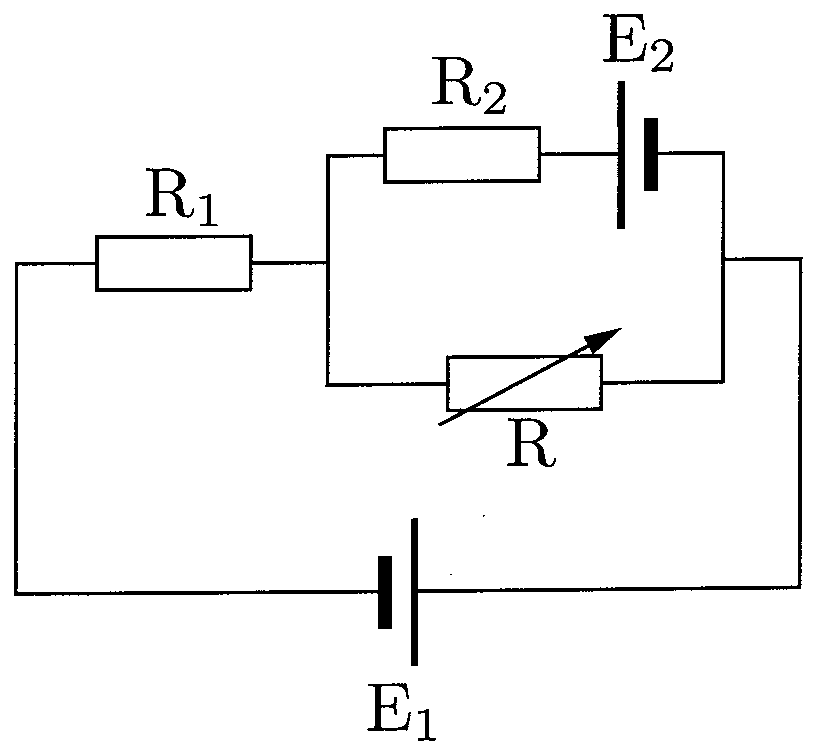
\includegraphics[keepaspectratio,width=42mm]{fig/n27_p72_zu.png}
\end{zuright}

\Mon[\Sitei]{ポテンシオメータ}

\begin{zuright}{50mm}
\hspace{1zw}右図はポテンシオメータと呼ばれる起電力測定のための回路である．$\mathrm{E}$，$\mathrm{R}$はある起電力および抵抗値を持つ電池および抵抗であり，$\mathrm{AB}$は長さ$l_0\U{m}$で一様な抵抗線，$\mathrm{E}_0$は起電力$V_0\U{V}$（既知）の標準電池，そして$\mathrm{E}_1$は起電力が未知の電池である．まずスイッチを$\mathrm{E}_0$側に入れて，検流計$\mathrm{G}$と抵抗線$\mathrm{AB}$の接触点$\mathrm{P}$を動かしていったところ，$\overline{\mathrm{AP}}=x_0\U{m}$になったとき検流計$\mathrm{G}$には電流が流れなくなった．次にスイッチを$\mathrm{E}_1$側に入れて検流計$\mathrm{G}$と抵抗線$\mathrm{AB}$の接触点$\mathrm{P}$を動かしていくと，$\overline{\mathrm{AP}}=x\U{m}$となったとき検流計$\mathrm{G}$には電流が流れなくなった．以上を元に，未知電池$\mathrm{E}_1$の起電力を求めよ．
\zusep
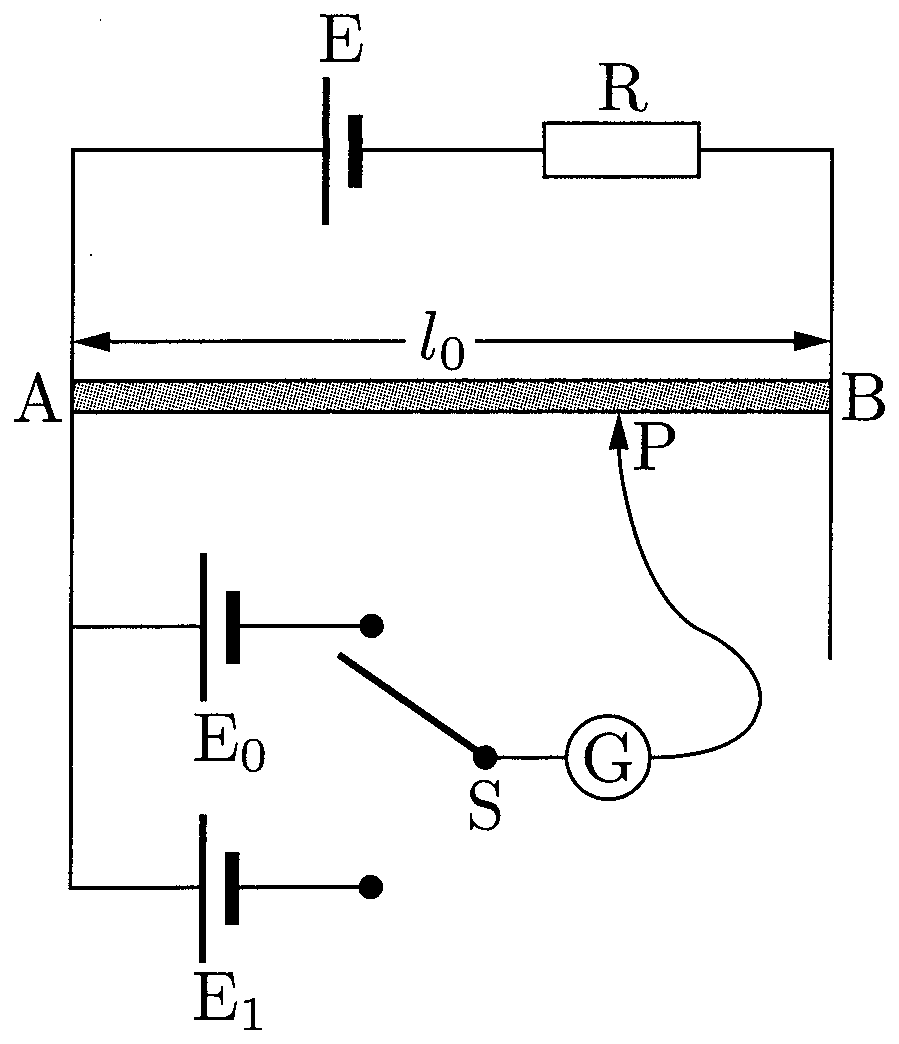
\includegraphics[keepaspectratio,width=46mm]{fig/n27_p73_zu.png}
\end{zuright}

\Mon{電池のする仕事と静電エネルギー}

\begin{zuright}{40mm}
\hspace{1zw}右図のように起電力$V\U{V}$の電池に電気容量$C\U{F}$のコンデンサーと電気抵抗をつないだ回路がある．はじめスイッチは開いており，コンデンサーには電荷が蓄えられていなかった．この状態からスイッチ$\mathrm{S}$を閉じ，十分時間を置いた．これについて以下の設問に答えよ．
\begin{komon}
\ko{1} 定常状態においてコンデンサーに蓄えられる静電エネルギー$W_1\U{J}$を求めよ．
\ko{2} この間に電池が供給したエネルギー$W_2\U{J}$を求めよ．
\ko{3} $W_1$と$W_2$の値は等しくない．この理由を簡単に説明せよ．
\end{komon}
\zusep
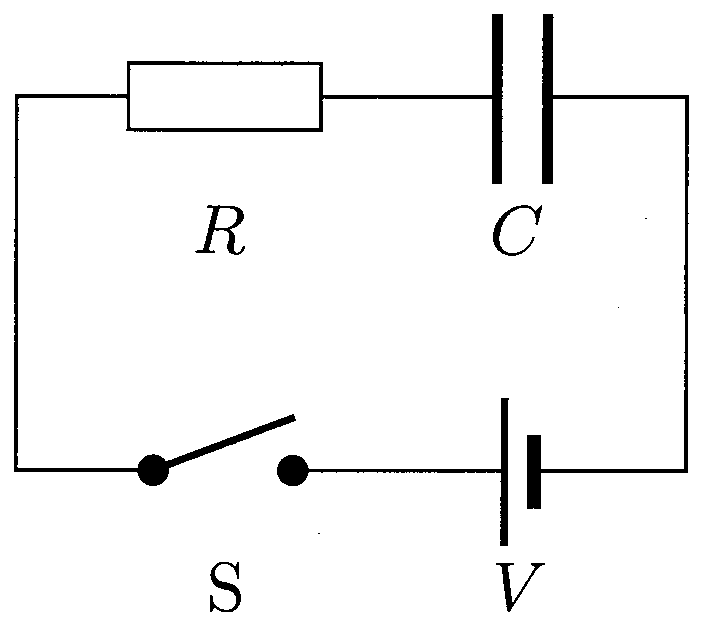
\includegraphics[keepaspectratio,width=36mm]{fig/n27_p74_zu.png}
\end{zuright}

\Mon[\Sitei]{抵抗・コンデンサー複合回路}

\begin{zuright}{50mm}
\hspace{1zw}内部抵抗の無視できる起電力$V\U{V}$の電池$\mathrm{E}$と抵抗値がそれぞれ$R$，$R$，$2R\U{\Omega}$の抵抗$\mathrm{R}_1$，$\mathrm{R}_2$，$\mathrm{R}_3$，そして電気容量$C\U{F}$のコンデンサー$\mathrm{C}$を右図のように接続した．スイッチ$\mathrm{S}$を閉じ，十分時間が経過したときについて，以下の設問に答えよ．
\begin{komon}
\ko{1} 各抵抗に流れる電流の強さを求めよ．
\ko{2} コンデンサーに蓄えられる電気量を求めよ．
\end{komon}
\zusep
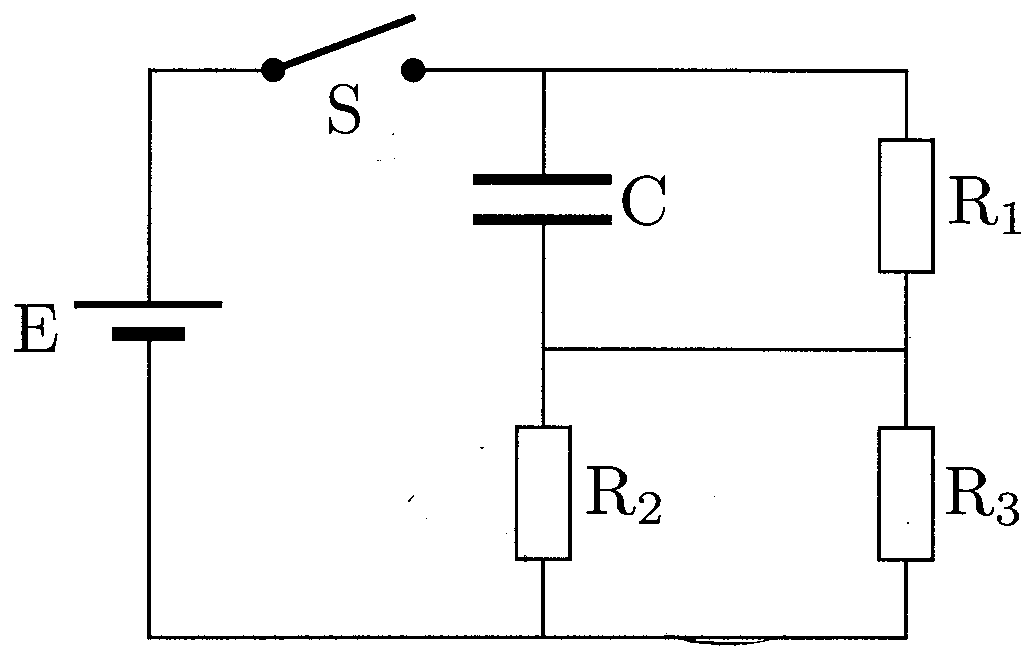
\includegraphics[keepaspectratio,width=46mm]{fig/n27_p75_zu.png}
\end{zuright}

\Mon{抵抗・コンデンサー複合回路}

\begin{zuright}{44mm}
\hspace{1zw}内部抵抗の無視できる起電力$12\U{V}$の電池$\mathrm{E}$と抵抗値がそれぞれ$4$，$8$，$12\U{\Omega}$の抵抗$\mathrm{R}_1$，$\mathrm{R}_2$，$\mathrm{R}_3$，電気容量$1$，$3$，$10\U{F}$のコンデンサー$\mathrm{C}_1$，$\mathrm{C}_2$，$\mathrm{C}_3$，そしてスイッチ$\mathrm{S}$を用いて右図のような回路を作った．はじめスイッチ$\mathrm{S}$は開いており，コンデンサー$\mathrm{C}_1$，$\mathrm{C}_2$，$\mathrm{C}_3$の極板上には電荷が蓄えられていなかったとして，以下の設問に答えよ．
\par
\hspace{1zw}まずスイッチ$\mathrm{S}$を開いたままで十分時間が経ったとき，
\begin{komon}
\ko{1} 抵抗$\mathrm{R}_1$を流れている電流の強さを求めよ．
\ko{2} コンデンサー$\mathrm{C}_1$に蓄えられている電気量を求めよ．
\end{komon}
\hspace{1zw}次にスイッチ$\mathrm{S}$を閉じて十分時間が経ったとき，
\begin{komon}
\ko{3} コンデンサー$\mathrm{C}_3$に蓄えられている電気量を求めよ．
\end{komon}
\zusep
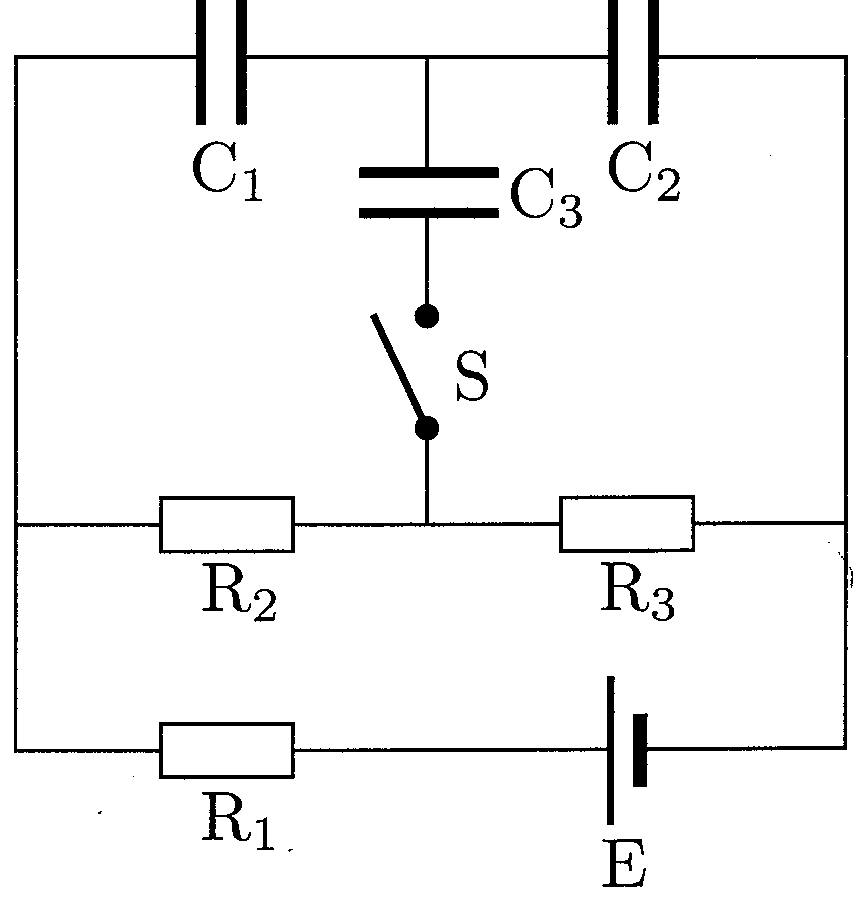
\includegraphics[keepaspectratio,width=40mm]{fig/n27_p76_zu.png}
\end{zuright}

\Mon[\Sitei]{非オーム抵抗}

\begin{zuright}{46mm}
\hspace{1zw}右図のグラフは，電球にかけた電圧の値と流れる電流の強さの関係を示している．この電球2個と，内部抵抗の無視できる起電力$6.0\U{V}$の電池，および抵抗を次のように接続した．それぞれの場合について，抵抗を流れる電流の強さを求めよ．
\zusep
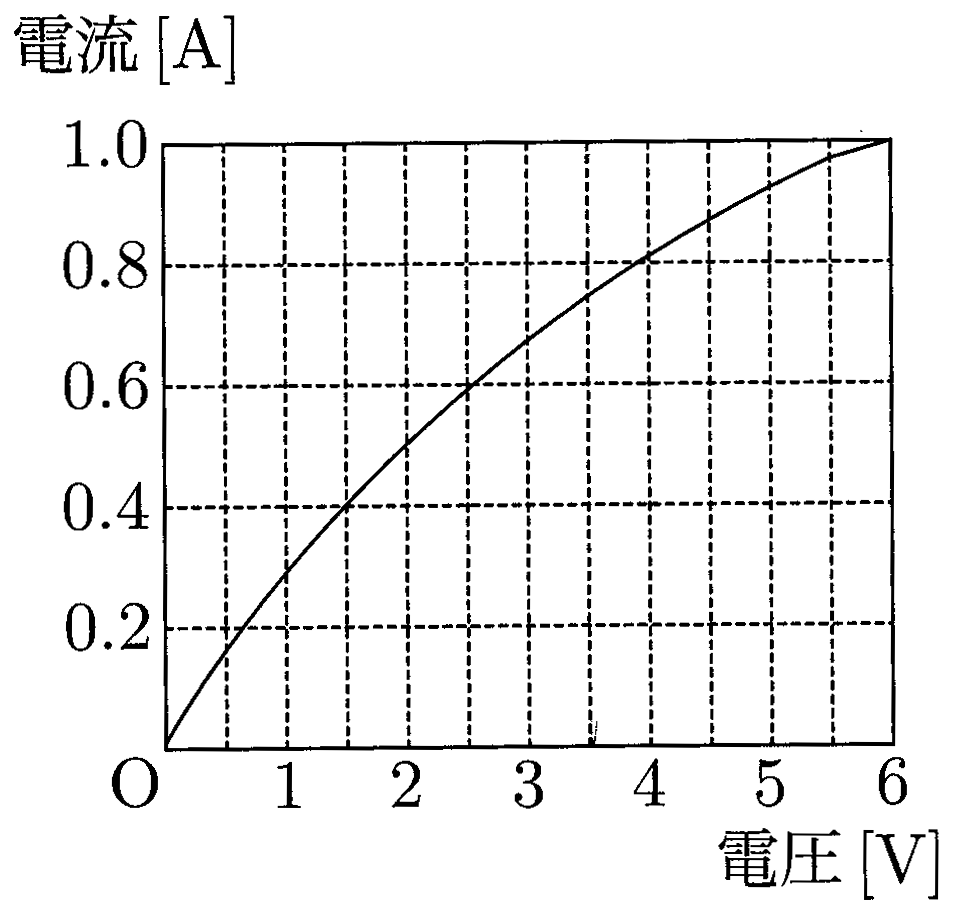
\includegraphics[keepaspectratio,width=44mm]{fig/n27_p77_graph.png}
\end{zuright}
\begin{center}
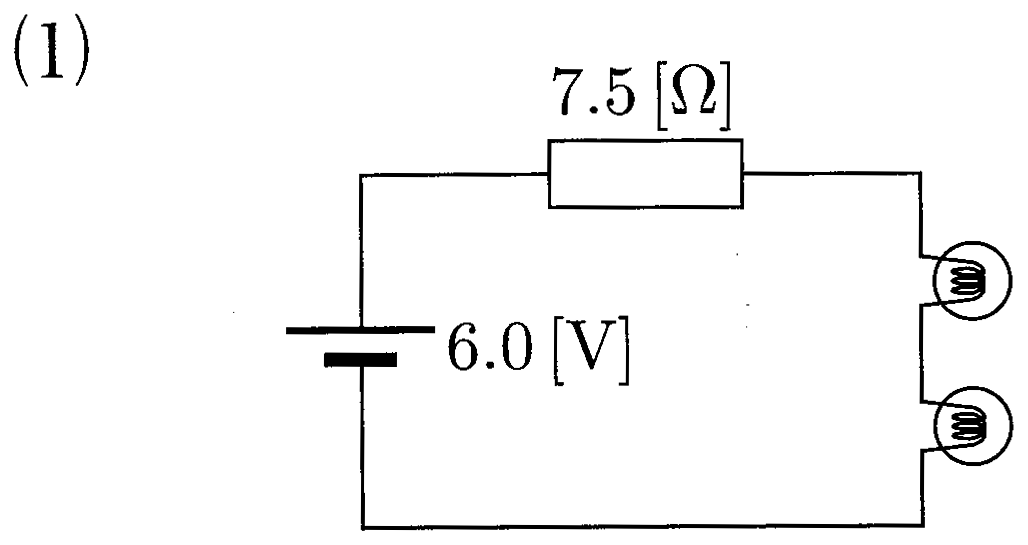
\includegraphics[keepaspectratio,width=54mm]{fig/n27_p77_zu1.png}\hspace{10mm}%
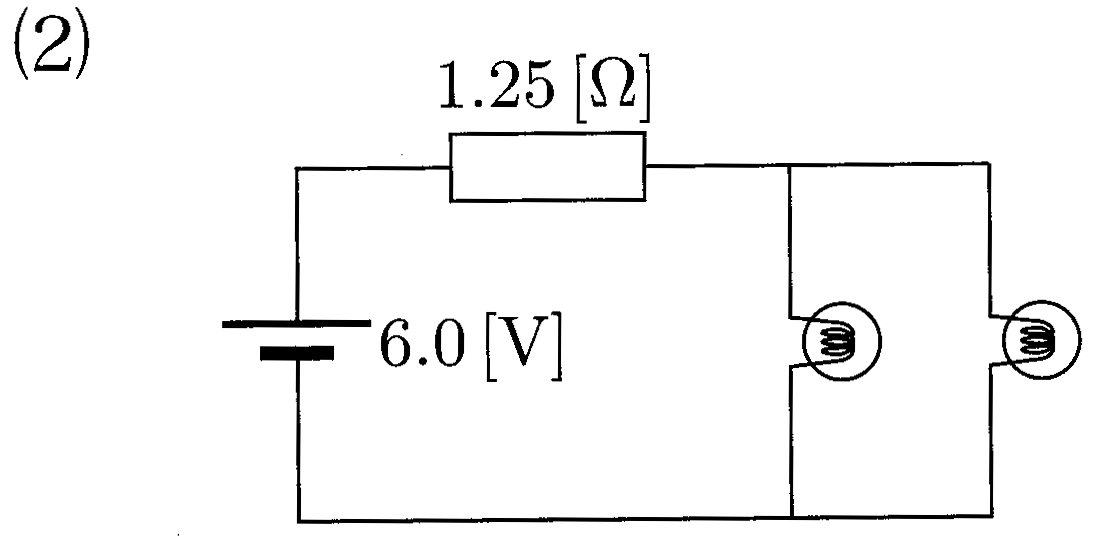
\includegraphics[keepaspectratio,width=57mm]{fig/n27_p77_zu2.png}
\end{center}

\filbreak
\Rank{C問題}

\Mon{非オーム抵抗の組み合わせ}

\begin{zuright}{44mm}
\hspace{1zw}右図のような電流-電圧特性曲線を持つ二つの電球$\mathrm{A}$，$\mathrm{B}$，および抵抗，内部抵抗の無視できる電池を用いて図のような回路(1)，(2)を作った．このとき，抵抗を流れる電流の強さをそれぞれ求めよ．
\zusep
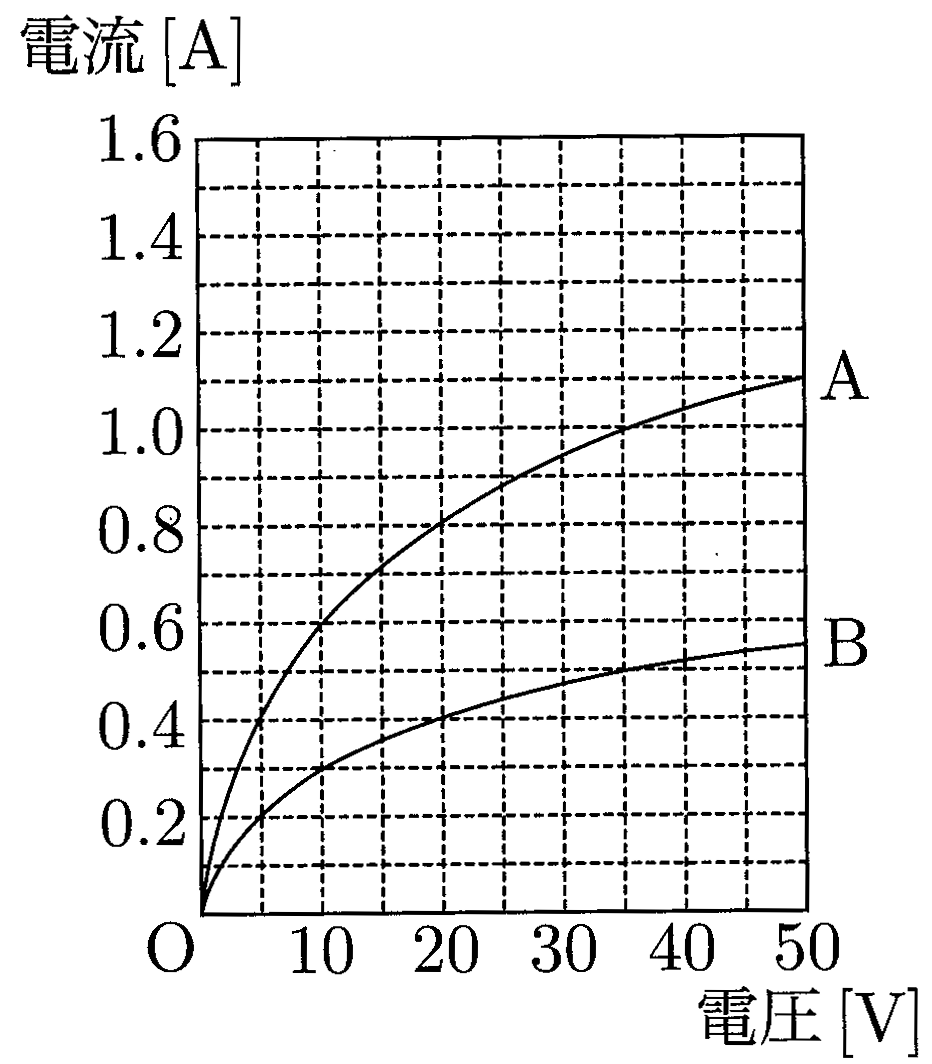
\includegraphics[keepaspectratio,width=44mm]{fig/n27_p78_graph.png}
\end{zuright}
\begin{center}
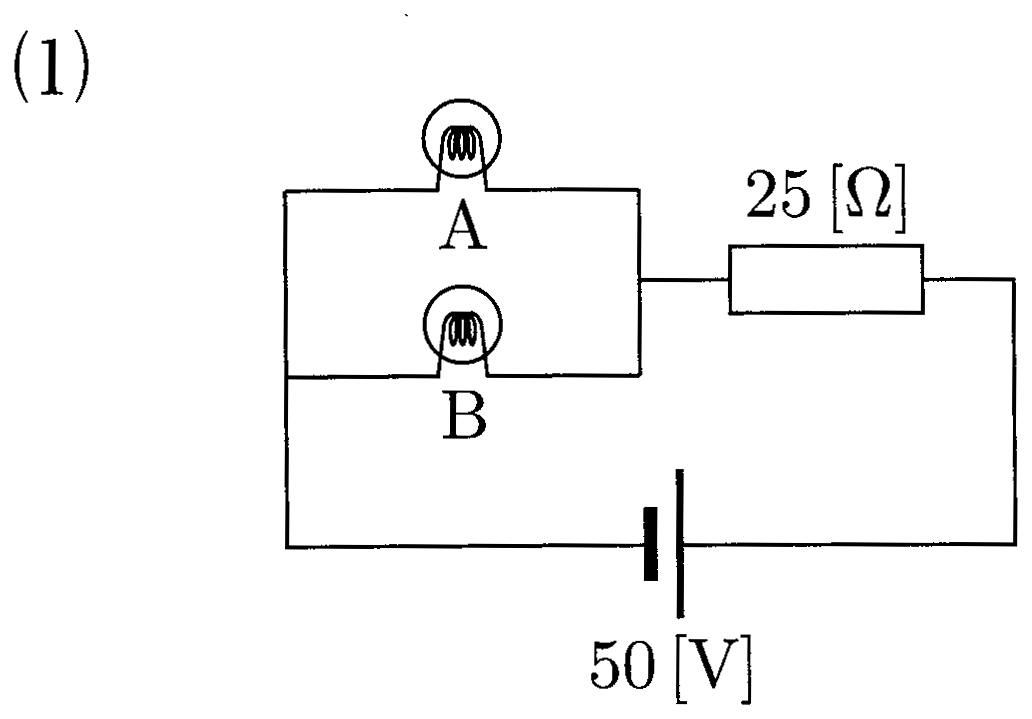
\includegraphics[keepaspectratio,width=54mm]{fig/n27_p78_zu1.png}\hspace{10mm}%
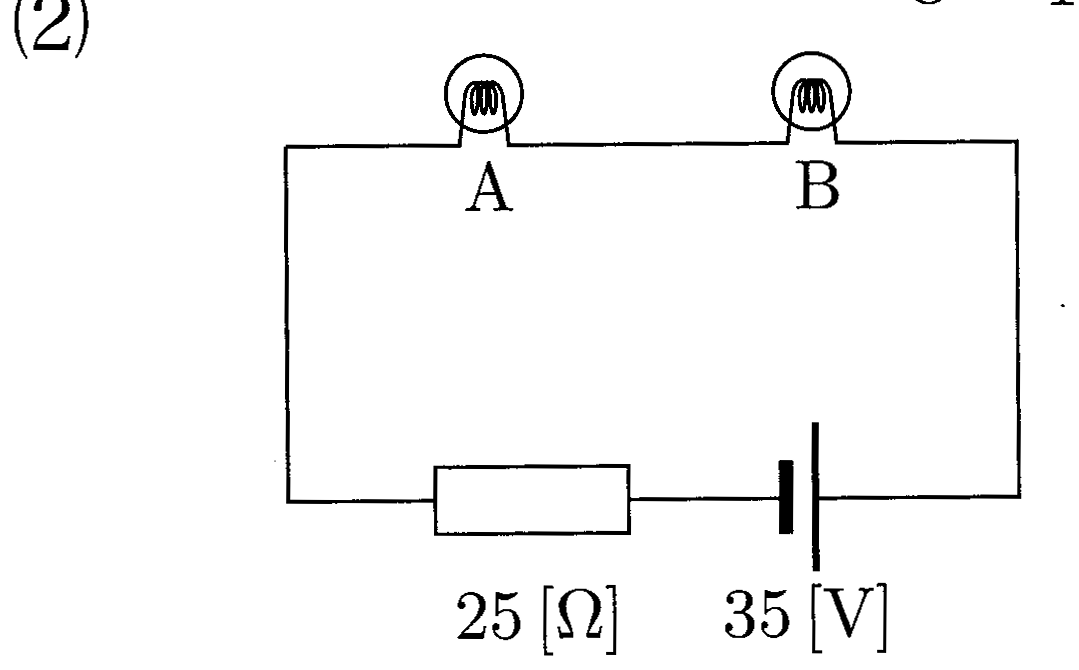
\includegraphics[keepaspectratio,width=56mm]{fig/n27_p78_zu2.png}
\end{center}

\Mon{抵抗値}

\begin{zuright}{44mm}
\hspace{1zw}右図のような電流-電圧特性曲線を持つ電球を，温度によらず一定の抵抗値を持つ三つのオーム抵抗，電池，検流計と共に図のような回路を作ったところ，検流計$\mathrm{G}$には電流が流れなかったという．このとき，この電球に流れる電流の強さはいくらか．
\zusep
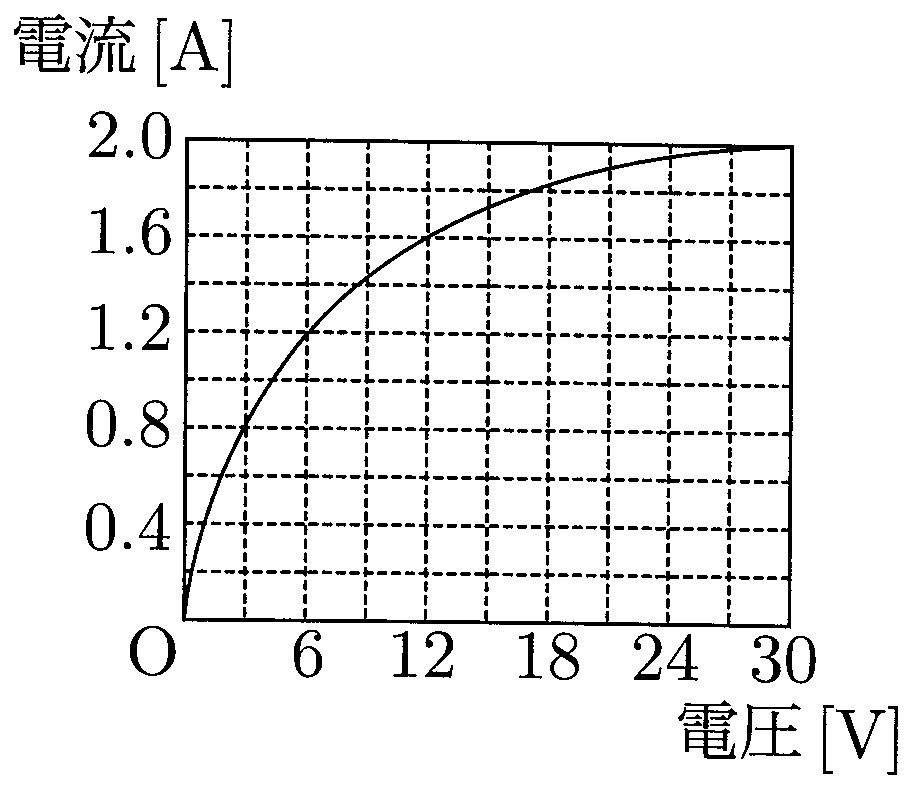
\includegraphics[keepaspectratio,width=42mm]{fig/n27_p79_graph.png}\\[2mm]
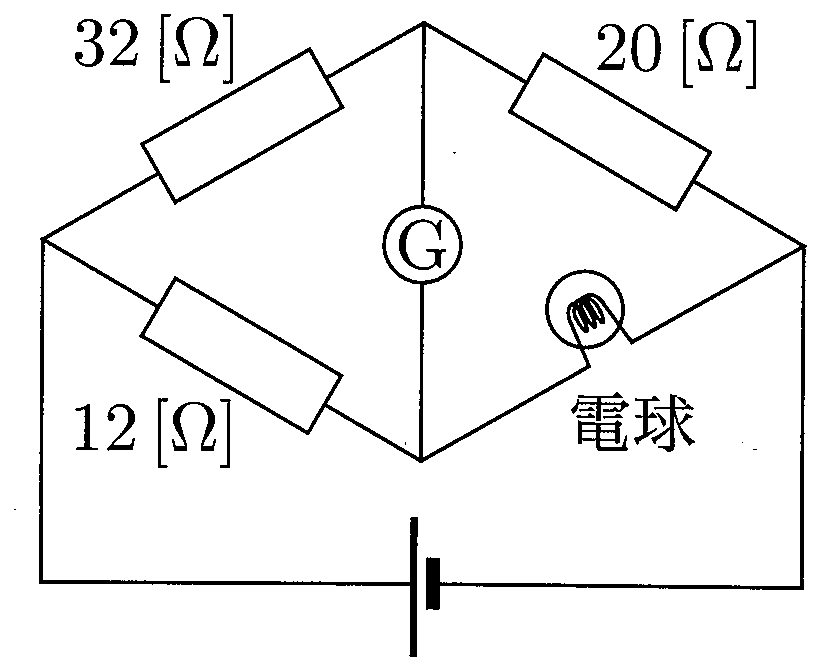
\includegraphics[keepaspectratio,width=40mm]{fig/n27_p79_zu.png}
\end{zuright}

\Mon{ダイオード}

\begin{zuright}{62mm}
\hspace{1zw}ダイオードとは，順方向に電圧をかけた場合にのみ電流を流し，逆方向に電圧をかけてもほとんど電流を流さない素子である．すなわち，図2のようにダイオードの二つの端子を$\mathrm{a}$，$\mathrm{b}$とし，$I$は端子$\mathrm{a}$から$\mathrm{b}$に流れるときを正，$V$は$\mathrm{b}$に対する$\mathrm{a}$の電位を正とするとき，$V>0$のときには$I>0$となるが，$V<0$のときにはほぼ$I=0$となるのがダイオードである．
\par
\hspace{1zw}今，ダイオードの端子電圧$V\U{V}$および順方向に流れる電流$I\U{A}$の関係が図1のようになっているダイオードを用意した．まずこのダイオードに抵抗値$R\U{\Omega}$の抵抗体をつなぎ，内部抵抗の無視できる起電力$E\U{V}$の電池を直列に図3のように接続した．これについて以下の設問に答えよ．
\zusep
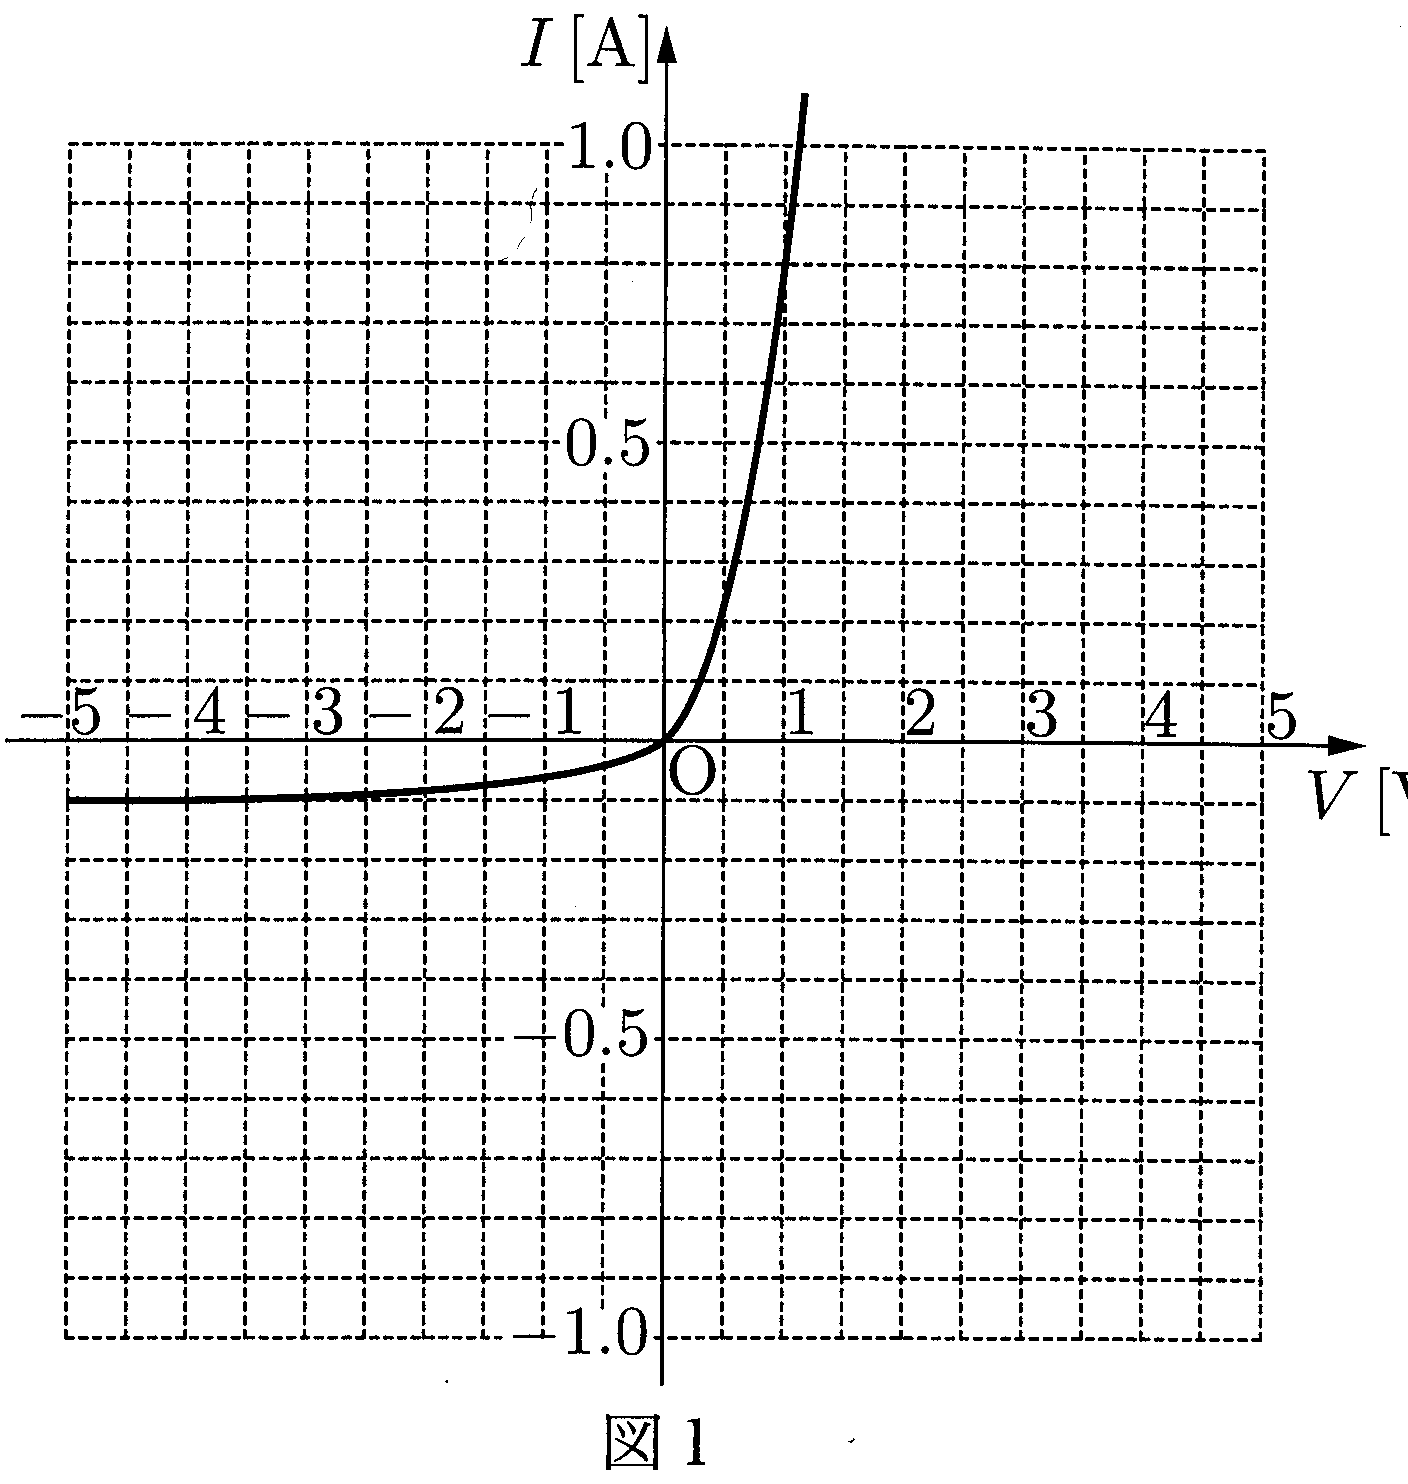
\includegraphics[keepaspectratio,width=58mm]{fig/n27_p80_zu1.png}
\end{zuright}
\begin{zuright}{62mm}
\begin{komon}
\ko{1} $E$，$V$，$I$，$R$の間に成り立つ関係式を求めよ．
\ko{2} $E=5\U{V}$，$R=5\U{\Omega}$のとき，$V$，$I$の値を求めよ．
\end{komon}
\hspace{1zw}次に，図3の回路において電池の正負の端子を逆にした．
\begin{komon}
\ko{3} $E$，$V$，$I$，$R$の間に成り立つ関係式を求めよ．
\ko{4} $E=5\U{V}$，$R=5\U{\Omega}$のとき，$V$，$I$の値を求めよ．
\end{komon}
\zusep
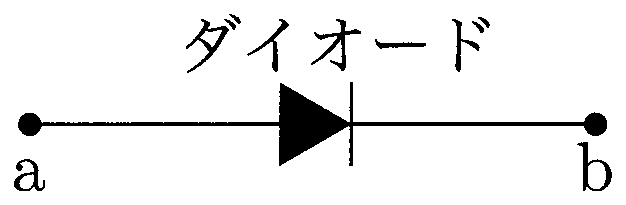
\includegraphics[keepaspectratio,width=34mm]{fig/n27_p80_zu2.png}\par{\small 図2}\\[2mm]
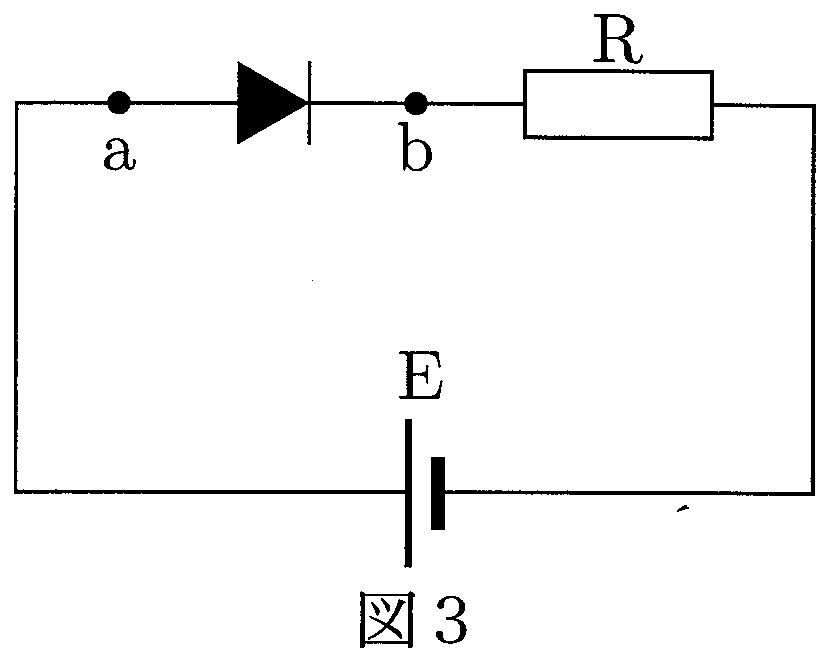
\includegraphics[keepaspectratio,width=44mm]{fig/n27_p80_zu3.png}
\end{zuright}

\newpage

%%%%%%%%%%%%%%%%%%%%  解答  %%%%%%%%%%%%%%%%%%%%
\KaiTitle{第27回　キルヒホッフの法則と直流回路}
\setlength{\columnseprule}{0.4pt}
\begin{multicols}{2}
\raggedcolumns

\Rank{A問題}
\MonN{69}{基本公式の確認}\par\nopagebreak
\begin{sisin}
電流計・電圧計の基本的な考え方を押さえること．電流計も電圧計も内部構造は同じで，いずれにも{\gtfamily 流せる電流に上限値がある}（電圧計の値は，（内部抵抗値）$\times$（電流の値）である）．題意の条件を満たすためにはどのように抵抗をつなげばよいのかを考えよ．

非オーム抵抗を利用した回路では，非オーム抵抗にかかる電圧と流れる電流がグラフとして与えられているので，これらを$V$，$I$とおいた上で回路のキルヒホッフの第二法則の式を立てる．
\end{sisin}
\KaiHead
\begin{komon}
\ko{1} 電流計のメーターには$5\U{mA}$の電流しか流せないので，$1\U{A}$の電流を流すためには図のように抵抗（分流器）を並列につなぎ，電流計のメーター部には$5\U{mA}$の電流しか流れなくてすむようにすればよい．
       \begin{center}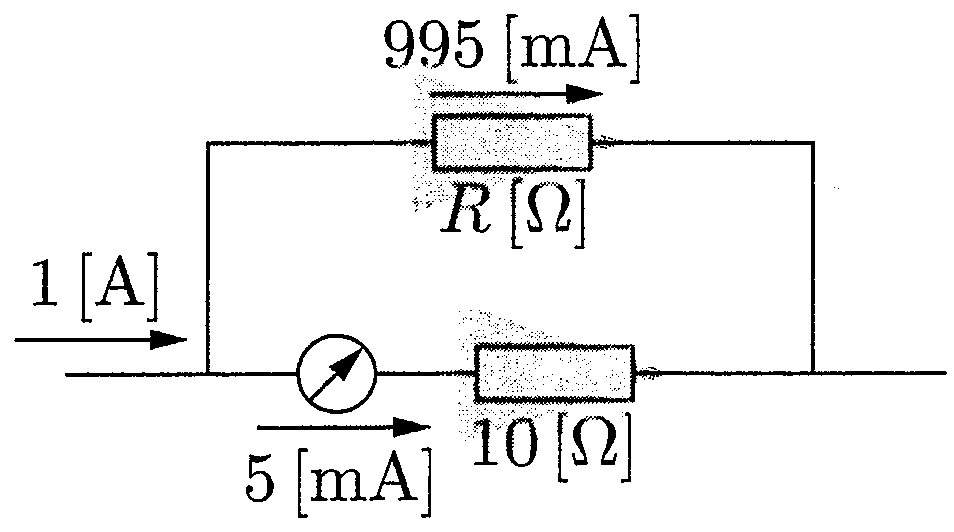
\includegraphics[keepaspectratio,width=52mm]{fig/n27_a69_zu1.png}\end{center}
       回路についてキルヒホッフの第二法則を用いて，
       \[0=R\cdot(995\times 10^{-3})-10\cdot(5\times 10^{-3})\]
       が成立するので，これより，
       \[R\fallingdotseq 0.050\U{\Omega}\Ans\]
\ko{2} 電圧計のメーターには$\dfrac{1}{1000}\U{A}$の電流しか流せないので，$100\U{V}$の電圧をかけるためには図のように抵抗（倍率器）を直列につなぎ，電圧計のメーター部には$\dfrac{1}{1000}\U{A}$の電流しか流れなくてすむようにすればよい．
       \begin{center}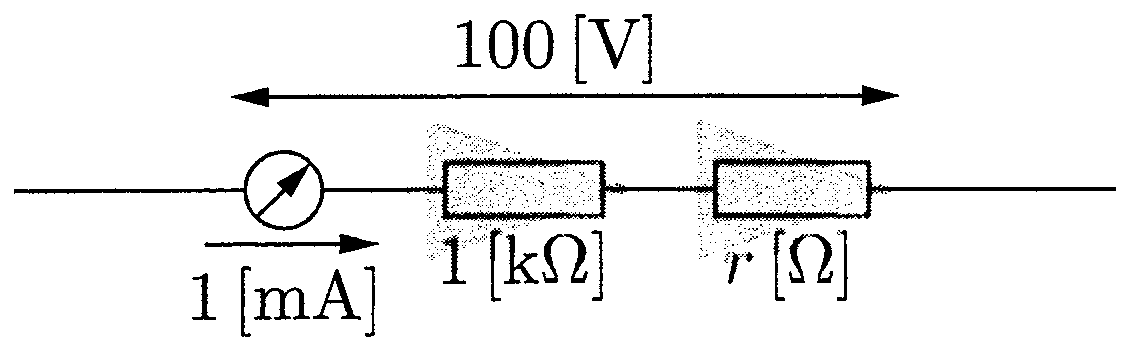
\includegraphics[keepaspectratio,width=56mm]{fig/n27_a69_zu2.png}\end{center}
       よって，
       \[100=1000\times\frac{1}{1000}+r\times\frac{1}{1000}\]
       が成立するように抵抗値を選べばよく，
       % 原本は「99 [KΩ]」（接頭語の k は小文字）．
       \[r=99000\U{\Omega}=99\U{k\Omega}\Ans\]
\ko{3} 電球にかかる電圧を$V\U{V}$，流れる電流を$I\U{A}$とすると，回路にキルヒホッフの第二法則を用いると，
       \[100=V+100\cdot I\]
       であり，整理すると
       \[I=-\frac{1}{100}V+1\]
       となる．これを$I$-$V$特性曲線に記入して曲線との交点を取ると，
       \[I=0.6\U{A}\Ans\]
       これが流れる電流に他ならない．
       \begin{center}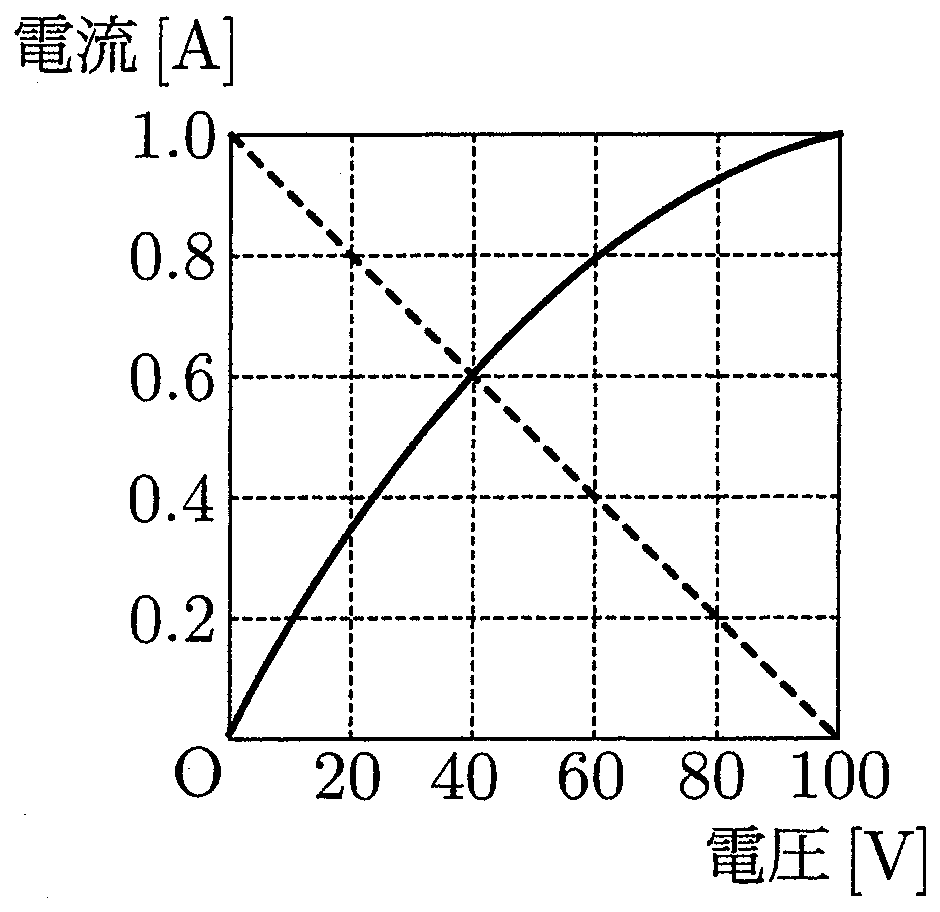
\includegraphics[keepaspectratio,width=48mm]{fig/n27_a69_graph.png}\end{center}
\end{komon}

\Rank{B問題}
\MonN{70}{キルヒホッフの法則の適用}\par\nopagebreak
\begin{sisin}
流れる電流の「向き」および，どちら向きに電圧降下が起こっているのかに注意しながら式を立てること．文字の置き方によっては電圧降下の向きが各抵抗ごとにバラバラになることもあるので注意せよ．

なお，キルヒホッフの第二法則を用いる閉ループは本問の場合は二つまで取ることができる（27.1）．解答に示した二つの式のいずれかの式のかわりに，外周に対してキルヒホッフの第二法則を利用してもよい．
% 原本は「（§33 B問題［25］注参照）」．旧回の参照なので 27.1 の本文に付け替えた．
\end{sisin}
\KaiHead
\begin{komon}
\ko{1} $\mathrm{A}$点に着目すると，上からは$I_1\U{A}$の電流が，右からは$I_2\U{A}$の電流が流入するので，キルヒホッフの第一法則より，$\mathrm{A}$点から下方向へは$(I_1+I_2)\U{A}$の電流が流れていく．よって，抵抗$\mathrm{R}_3$に流れる電流は，
       \[\text{右向きに，強さ}\ I_1+I_2\U{A}\Ans\]
       \begin{center}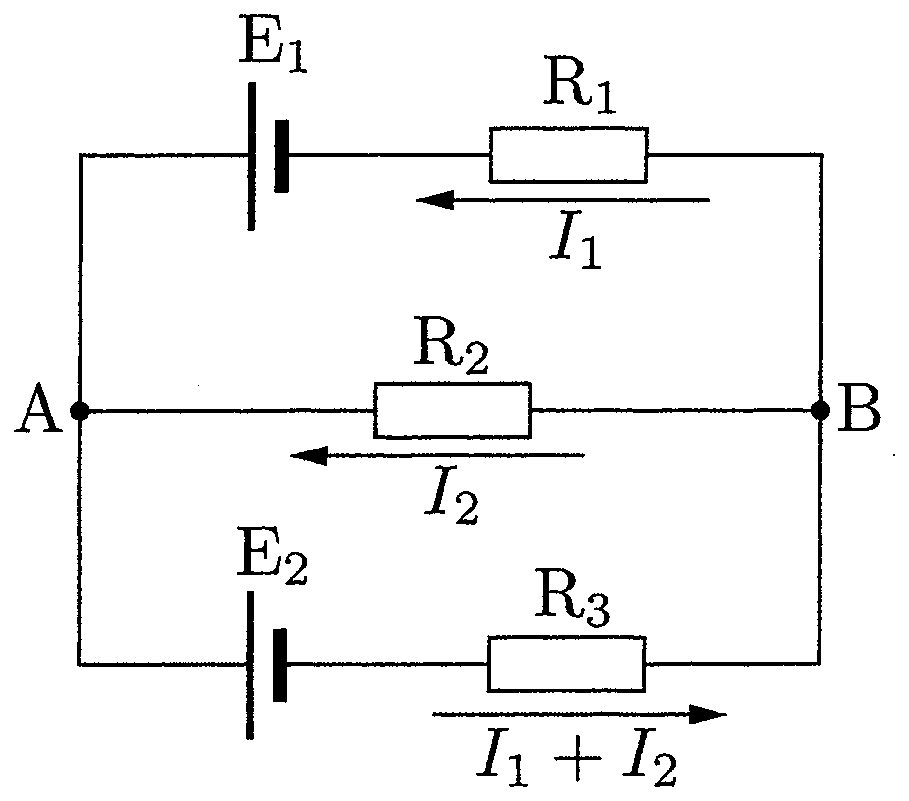
\includegraphics[keepaspectratio,width=50mm]{fig/n27_a70_zu1.png}\end{center}
       \begin{chuu}
       $\mathrm{B}$点に着目して考えてもよい．$\mathrm{B}$点に着目すると，上へは$I_1\U{A}$の電流が，左へは$I_2\U{A}$の電流が流出するので，キルヒホッフの第一法則より，$\mathrm{B}$点には下方向から$I_1+I_2\U{A}$の電流が流れ込んでいなければならない．このことから同じ答えを得ることができる．
       \end{chuu}
\ko{2} (1)の電流分布を元に各抵抗における電圧降下を考えると次図のようになる．
       \begin{center}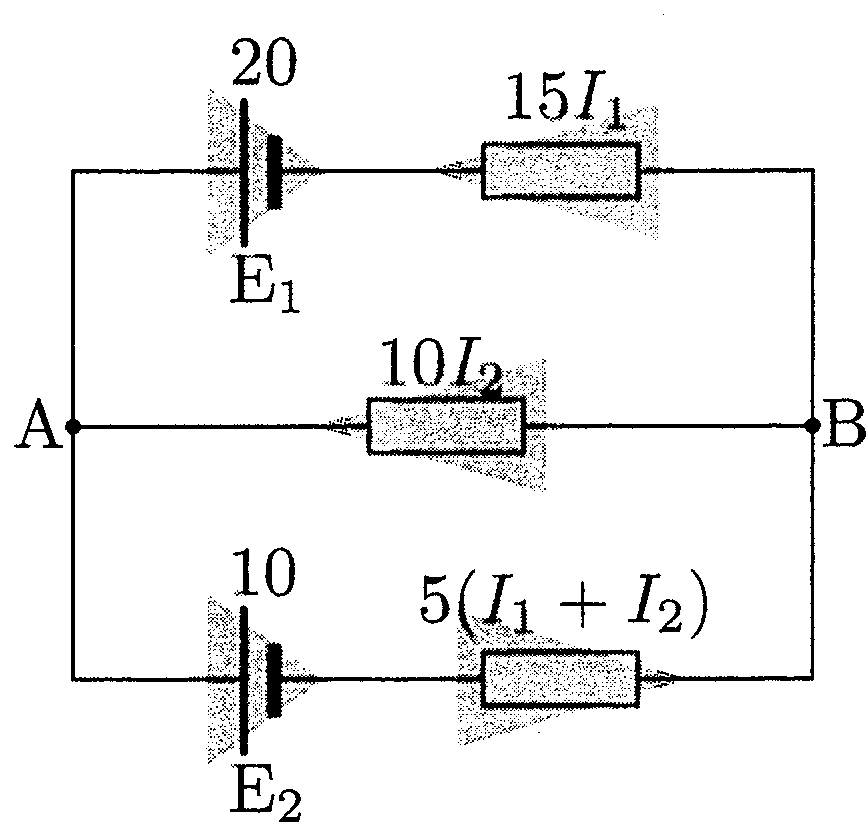
\includegraphics[keepaspectratio,width=50mm]{fig/n27_a70_zu2.png}\end{center}
       よって，上側および下側の各閉ループに対してキルヒホッフの第二法則より立式すると，
       \[\left\{\begin{aligned}
         20&=15I_1-10I_2\\
         -10&=5(I_1+I_2)+10I_2
       \end{aligned}\right.\Ans\]
       \begin{bekkai}
       上の二つの式のいずれかの代わりとして，外周に対してキルヒホッフの第二法則を用いて
       \[20-10=5(I_1+I_2)+15I_1\]
       を答えとしてもよい．
       \end{bekkai}
\ko{3} 以上2式を解くと，
       \[I_1=\frac{8}{11}\fallingdotseq 0.73\U{A},\quad I_2=-\frac{10}{11}\fallingdotseq -0.91\U{A}\]
       であり，また
       \[I_1+I_2=-\frac{2}{11}\fallingdotseq -0.18\U{A}\]
       である．求めた値が負値であったということは，最初に仮定した向きが逆であったことを意味する．よって，
       \[\left\{\begin{aligned}
         &\mathrm{R}_1\text{：左向きに強さ}\ 0.73\U{A}\\
         &\mathrm{R}_2\text{：右向きに強さ}\ 0.91\U{A}\\
         &\mathrm{R}_3\text{：左向きに強さ}\ 0.18\U{A}
       \end{aligned}\right.\Ans\]
\end{komon}

\MonN{71}{メートルブリッジ}\par\nopagebreak
\begin{sisin}
本問のような，一様な抵抗線を接点によって2分割するようなタイプの問題では，右側，左側をそれぞれ一つの抵抗とみなして回路図を書き換えてやると分かりやすい．本問においてこれを行うと，ただのホイートストンブリッジ回路であることが分かる．
\end{sisin}
\KaiHead
未知抵抗$\mathrm{R}$の抵抗値を$R\U{\Omega}$とする．$\mathrm{AP}$，$\mathrm{PB}$の抵抗値をそれぞれ$R_{\mathrm{AP}}\U{\Omega}$，$R_{\mathrm{PB}}\U{\Omega}$とおく．抵抗線の抵抗率を$\rho\U{\Omega\cdot m}$，断面積を$S\U{m^2}$とすると，
\[R_{\mathrm{AP}}=\rho\frac{x}{S}\U{\Omega},\qquad R_{\mathrm{PB}}=\rho\frac{l_0-x}{S}\U{\Omega}\]
であり，回路図を書き換えると次図のようになる．
\begin{center}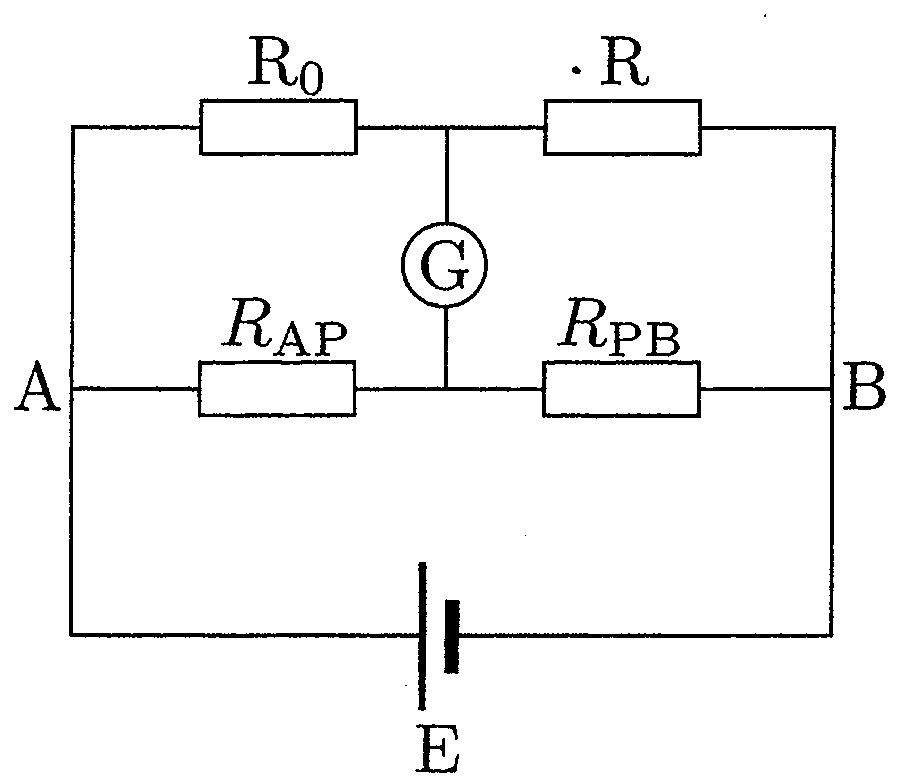
\includegraphics[keepaspectratio,width=48mm]{fig/n27_a71_zu.png}\end{center}
よって，この回路はホイートストンブリッジ回路と同じになっており，$\mathrm{AP}=x\U{m}$となったときに$\mathrm{G}$に電流が流れなくなったのだから，ブリッジ回路の特性より，このとき
\[R_0:R_{\mathrm{AP}}=R:R_{\mathrm{PB}}\]
が成立する．よってこれを解くと，
\[R=\frac{R_{\mathrm{PB}}}{R_{\mathrm{AP}}}R_0=\frac{l_0-x}{x}R_0\U{\Omega}\Ans\]

\MonN[\Sitei]{72}{可変抵抗を用いた回路}\par\nopagebreak
\begin{sisin}
可変抵抗を用いている回路であっても考え方・攻め方は［70］と全く同じである．［70］と違い，本問は誘導がないので，抵抗$\mathrm{R}_1$に流れる電流か，$\mathrm{R}_2$に流れる電流かのいずれかを適当な文字で設定する．電池の向きを考えれば電流はおそらく$\mathrm{R}_1$，$\mathrm{R}_2$ともに左向きに流れると考えられるが，右向きに文字を設定した場合でも同じ答え$I(x)\U{A}$が得られる．

消費電力の式は，$P=RI^2=IV=\dfrac{V^2}{R}$と3通りの書き方があるが，どの文字が既知であるかを考えて使い分けること．(2)では，この抵抗にかかる電圧については$xI(x)$を計算しなくてはならないが，流れる電流$I(x)$は既知であるから，$P=RI^2$を用いて計算する．

本問のような消費電力の最大値を求めるタイプの問題では，相加平均・相乗平均の関係式をうまく利用すると簡単に求められる場合がある（第26回の練習［67］）．
\end{sisin}
\KaiHead
\begin{komon}
\ko{1} 抵抗$\mathrm{R}_2$に流れる電流を，左向きに$i\U{A}$であると置くと，キルヒホッフの第一法則より抵抗$\mathrm{R}_1$に流れる電流は左向きに$I(x)+i\U{A}$であり，各抵抗での電圧降下は次図の通りとなる．
       \begin{center}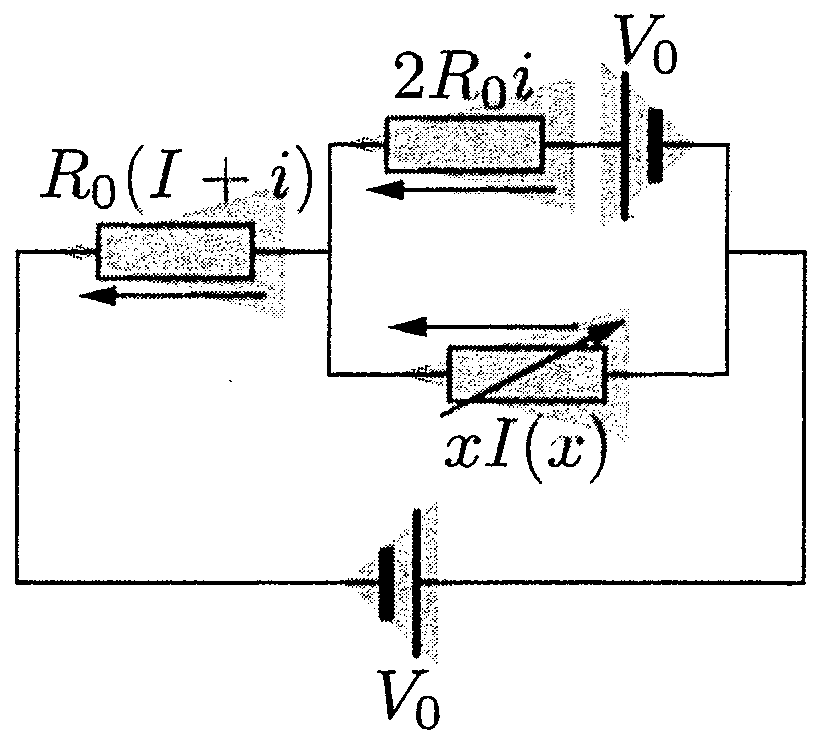
\includegraphics[keepaspectratio,width=50mm]{fig/n27_a72_zu.png}\end{center}
       この回路の上側・下側の各ループに対してキルヒホッフの第二法則を用いて立式すると，
       \[\begin{aligned}
         V_0&=2R_0i-xI(x)\\
         V_0&=xI(x)+R_0\{I(x)+i\}
       \end{aligned}\]
       である．以上2式を整理して$i$を消去し，$I(x)$を求めると，
       \[I(x)=\frac{V_0}{3x+2R_0}\U{A}\Ans\]
\ko{2} 可変抵抗$\mathrm{R}$で消費する電力$P(x)\U{W}$は，
       \[P(x)=x\{I(x)\}^2=\frac{x}{(3x+2R_0)^2}V_0^2\U{W}\]
       である．ここで，
       \[\frac{x}{(3x+2R_0)^2}V_0^2=\frac{V_0^2}{\Bigl(3\sqrt{x}+\dfrac{2R_0}{\sqrt{x}}\Bigr)^2}\]
       となる．可変抵抗$\mathrm{R}$の抵抗値$x\U{\Omega}$を変化させるとき，$P(x)\U{W}$が最大となるのはこの式の分母が最小となるときであるが，分母の括弧内に対して相加平均・相乗平均の関係を適用すると，
       \[3\sqrt{x}+\frac{2R_0}{\sqrt{x}}\geqq 2\sqrt{3\sqrt{x}\times\frac{2R_0}{\sqrt{x}}}=2\sqrt{6R_0}\]
       であり，この式の等号が成立するのは$3\sqrt{x}=\dfrac{2R_0}{\sqrt{x}}$のとき，すなわち$x=\dfrac{2}{3}R_0\U{\Omega}$のときである．以上より，可変抵抗$\mathrm{R}$での消費電力が最大になるのは
       \[x=\frac{2}{3}R_0\U{\Omega}\Ans\]
\end{komon}
\begin{bekkai}
相加平均・相乗平均の関係を思いつけない場合には，
\[P(x)=\frac{x}{(3x+2R_0)^2}V_0^2\U{W}\]
を微分するしかない．上式を微分すると，
\[\frac{d}{dx}P(x)=\frac{2R_0-3x}{(3x+2R_0)^3}V_0^2\]
となるので，$P(x)$は$x=\dfrac{2}{3}R_0\U{\Omega}$で最大値を取る．
\end{bekkai}

\MonN[\Sitei]{73}{ポテンシオメータ}\par\nopagebreak
\begin{sisin}
電池の起電力を測定するためには，電池の両端子間に電圧計をつないでその読みを測ればよい，と考える人も多いだろうが，実際にはこの方法では精密な起電力を測定することはできない．なぜなら，電圧計を接続すると電池から微量ではあるが電流が流れるため，電圧計の読みは電池の起電力から内部抵抗での電圧降下分を差し引いた値となってしまうからである．そのため，電池の起電力を測定するためには，本問のように電池に電流が流れないようにした状態で電圧を測定する必要があり，この装置をポテンシオメータと呼ぶ（27.2）．電流が流れないときの電流分布を考えればあっさりと解くことが出来る問題である．
\end{sisin}
\KaiHead
検流計$\mathrm{G}$に電流が流れていないときには下側の電池に電流が流れていないので，上側のループ部分だけで電流が流れている．$\mathrm{AP}$，$\mathrm{PB}$の抵抗値をそれぞれ$R_{\mathrm{AP}}\U{\Omega}$，$R_{\mathrm{PB}}\U{\Omega}$とおき，抵抗線の抵抗率を$\rho\U{\Omega\cdot m}$，断面積を$S\U{m^2}$とすると，
\[R_{\mathrm{AP}}=\rho\frac{\overline{\mathrm{AP}}}{S}\U{\Omega},\qquad R_{\mathrm{PB}}=\rho\frac{\overline{\mathrm{PB}}}{S}\U{\Omega}\]
であり，電池から内部抵抗を分けて回路図を書き換えると次図のようになる．
\begin{center}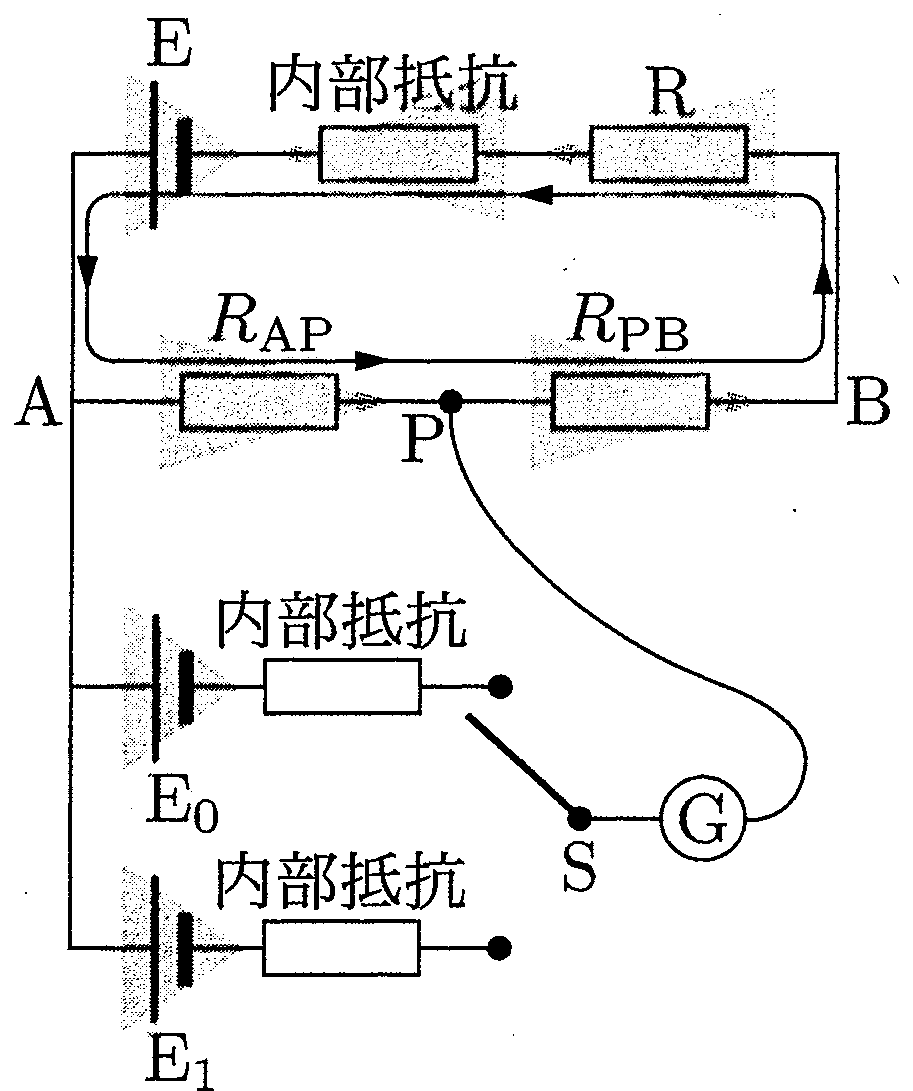
\includegraphics[keepaspectratio,width=50mm]{fig/n27_a73_zu.png}\end{center}
このとき，電池の内部抵抗には電流が流れないため，内部抵抗では電圧降下がない．よって，下側の電池の起電力は，$\mathrm{AP}$部分の抵抗における電圧降下と完全に一致することになる．

今，スイッチを$\mathrm{E}_0$に入れた場合には$\overline{\mathrm{AP}}=x_0\U{m}$としたときに上述した状態になる．電池$\mathrm{E}$の起電力を$E\U{V}$，$\mathrm{R}$の抵抗値を$R\U{\Omega}$，電池の内部抵抗を$r\U{\Omega}$とすると，上側のループを流れる電流$I\U{A}$は，
\[I=\frac{E}{R+r+R_{\mathrm{AP}}+R_{\mathrm{PB}}}=\frac{E}{R+r+\rho\dfrac{l_0}{S}}\U{A}\]
となり，標準電池の起電力$V_0\U{V}$は
\[V_0=R_{\mathrm{AP}}\cdot I=\rho\frac{x_0}{S}\cdot\frac{E}{R+r+\rho\dfrac{l_0}{S}}\U{V}\]
と表される．

また，スイッチを$\mathrm{E}_1$に入れた場合には$\overline{\mathrm{AP}}=x\U{m}$としたときに上述した状態になる．このとき上側のループを流れる電流$I\U{A}$は先ほどと全く同じである．これより，未知電池$\mathrm{E}_1$の起電力$V\U{V}$は
\[V=R_{\mathrm{AP}}\cdot I=\rho\frac{x}{S}\cdot\frac{E}{R+r+\rho\dfrac{l_0}{S}}\U{V}\]
となり，先の$V_0\U{V}$の式と組み合わせて解くと，
\[V=\frac{x}{x_0}V_0\U{V}\Ans\]

\MonN{74}{電池のする仕事と静電エネルギー}\par\nopagebreak
\begin{sisin}
定常状態ではコンデンサーに$V\U{V}$の電圧がかかって$Q=CV\U{C}$の電荷が蓄えられる．このことを用いてコンデンサーに蓄えられる静電エネルギーを求めよ．

電池のした仕事については次のように考えよ．電池の負極側から正極側へ$\varDelta q\U{C}$の電荷が通過したとき，この電荷は電位が$V\U{V}$だけ高い点に移動したことになるので，$\varDelta q\cdot V\U{J}$だけエネルギーが増加していることになる．よって，このときには電池はそのエネルギーの増分$\varDelta q\cdot V\U{J}$だけ電荷に対して仕事をしていることになる．

また逆に，電池の正極側から負極側へ$\varDelta q\U{C}$の電荷が通過したときには電荷は電位が$V\U{V}$だけ低い点に移動したことになるので，$\varDelta q\cdot V\U{J}$だけエネルギーを失い，その分が電池に蓄えられることになる（これは充電の現象である）．
\end{sisin}
\KaiHead
\begin{komon}
\ko{1} スイッチを閉じてから十分時間がたつとコンデンサーには$V\U{V}$の電圧がかかるので，このとき蓄えられている電荷$Q\U{C}$は，$Q=CV$である．よって，コンデンサーに蓄えられる静電エネルギーは，
       \[W_1=\frac{Q^2}{2C}=\frac{1}{2}CV^2\U{J}\Ans\]
\ko{2} スイッチを閉じてからこの状態に至るまでに電池を通過した電荷を考えると，コンデンサーの右側極板から$Q\U{C}$の電荷が，電池，スイッチ，抵抗を通過してコンデンサーの左側極板へと移動してコンデンサーに電荷が蓄えられた．よって，電池の負極から正極に向かって通過した電気量は$Q\U{C}$．電池は，これだけの電荷を負極側から$V\U{V}$だけ電位の高い正極側へと持ち上げたことになるから，電池がした仕事は電荷のエネルギー増加を考えて，
       \[W_2=QV=CV^2\U{J}\Ans\]
\ko{3} 以上より，$W_2-W_1>0$となり，電池がした仕事すべてがコンデンサーにエネルギーとして蓄えられてはいないことが分かる．これは，{\gtfamily 電荷が移動する際に，抵抗から熱エネルギー（ジュール熱）として散逸したからである}．\Ans
\end{komon}
\begin{bsHosoku}{参考}
抵抗に電流が流れる（電荷が通過する）と熱が発生する．これをジュール熱といい，第26回で学んだ．散逸したエネルギー$W_2-W_1=\dfrac{1}{2}CV^2$は抵抗値によらない（27.3）．
% 原本は「詳しくは§34にて学習する」（旧回の参照）．
\end{bsHosoku}

\MonN[\Sitei]{75}{抵抗・コンデンサー複合回路}\par\nopagebreak
\begin{sisin}
電流がコンデンサー極板に流れ込むことによって電荷が溜まるので，定常状態，すなわち，十分に時間がたって極板上の電荷が一定値になったときにはコンデンサーへは電流が流入しない．このことを利用して電流分布を考え，キルヒホッフの第二法則を適用しよう．

なお定常状態とは，回路がある一定の状態になって見かけ上，変化がなくなった状態のことを言うが，本問のような回路の場合にはコンデンサーについては溜まる電荷が一定となって電流が流れ込まなくなり，また抵抗については流れる電流が一定値になった状態がこの定常状態である．見かけ上変化がなくなった状態とは流れる電流が$0$の状態という意味ではないので注意．
\end{sisin}
\KaiHead
\begin{komon}
\ko{1} このときに抵抗$\mathrm{R}_2$，$\mathrm{R}_3$に流れる電流を下向きに$i$，$I\U{A}$とおく．定常状態ではコンデンサー上の電気量は一定値となるのでコンデンサーへは電流が流れ込まない．よって回路の電流分布は次図のようになる．
       \begin{center}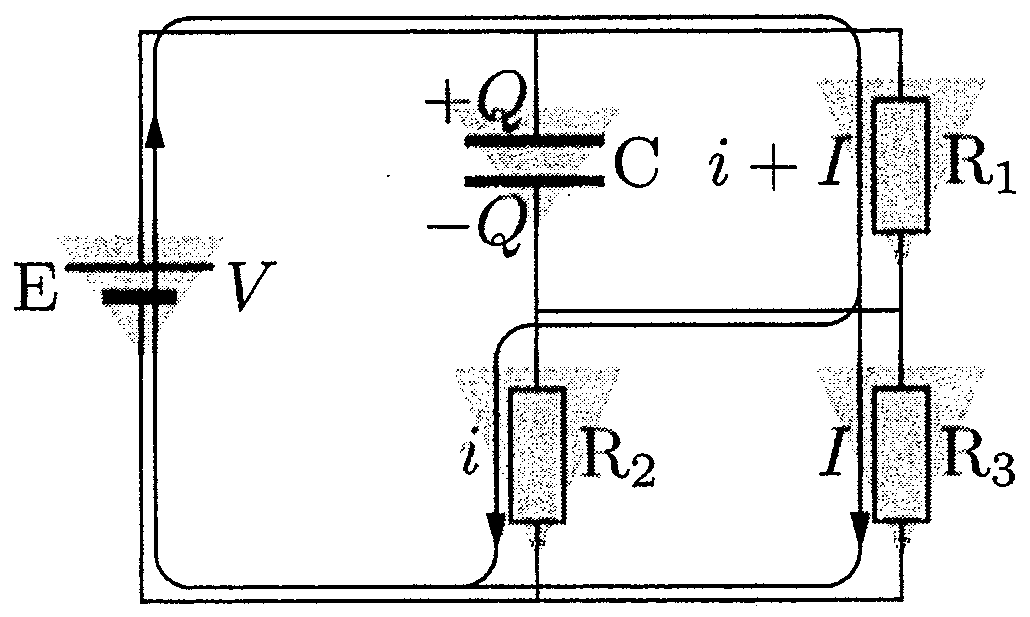
\includegraphics[keepaspectratio,width=52mm]{fig/n27_a75_zu1.png}\end{center}
       前図より，抵抗$\mathrm{R}_1$に流れる電流はキルヒホッフの第一法則より$i+I\U{A}$である．また抵抗$\mathrm{R}_1$での電圧降下の向きを考えて，コンデンサー$\mathrm{C}$の上側極板の帯電量を$+Q\U{C}$とおく．回路に対してキルヒホッフの第二法則を用いて立式すると，
       \[\begin{aligned}
         &\text{右下ループ：}\ 0=R\cdot i-2R\cdot I\\
         &\text{外周ループ：}\ V=R\cdot(i+I)+2R\cdot I\\
         &\text{右上ループ：}\ 0=R\cdot(i+I)-\frac{Q}{C}
       \end{aligned}\]
       となる．上の二つの式を組み合わせて解くと，
       \[I=\frac{V}{5R}\U{A},\qquad i=\frac{2V}{5R}\U{A}\]
       であるから，各抵抗に流れる電流は，
       \[\left\{\begin{aligned}
         &\mathrm{R}_1\text{：下向きに強さ}\ I+i=\frac{3V}{5R}\U{A}\\
         &\mathrm{R}_2\text{：下向きに強さ}\ i=\frac{2V}{5R}\U{A}\\
         &\mathrm{R}_3\text{：下向きに強さ}\ I=\frac{V}{5R}\U{A}
       \end{aligned}\right.\Ans\]
\ko{2} また(1)で立てた三つ目の式を解くと，
       \[Q=C\cdot R\cdot(i+I)=\frac{3}{5}CV\U{C}\Ans\]
\end{komon}
\begin{chuu}
(1)で，左側のループではなく外周ループに対するキルヒホッフの第二法則を利用したが，これは次のような理由による．抵抗とコンデンサーの複合回路において，定常状態ではコンデンサーに電流は流れ込まないので，電流分布にだけ着目するのであればコンデンサーの部分はなくてもよい（27.4）．つまり，回路の電流分布はコンデンサーを取り除いた次図の回路の場合と全く同一になる．
\begin{center}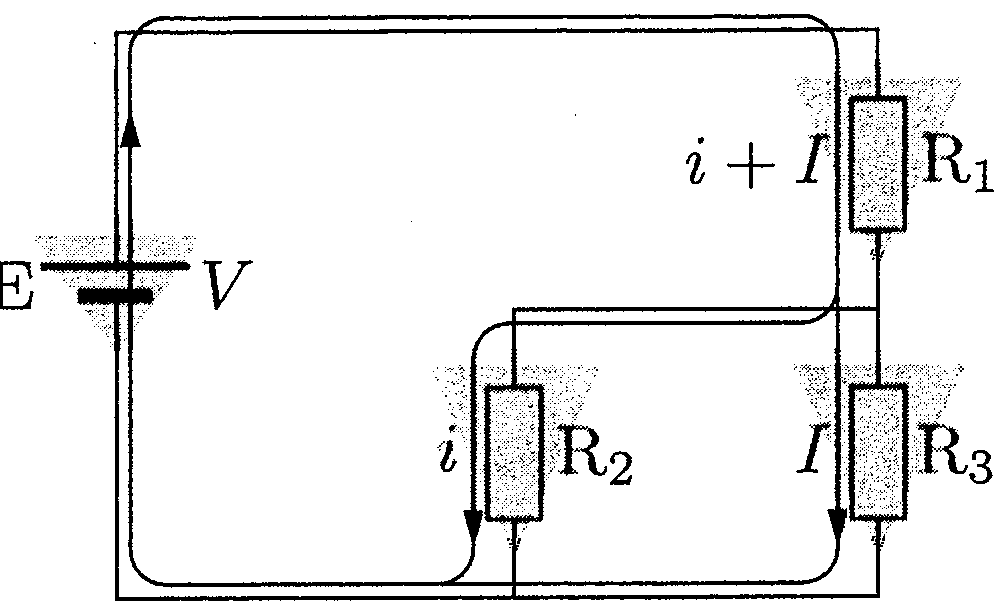
\includegraphics[keepaspectratio,width=52mm]{fig/n27_a75_zu2.png}\end{center}
よって，まずこの回路図に右下ループ・外周ループの二つの式を立てて回路の電流分布を先に決めてしまい，そして後から右上ループの式を利用してコンデンサーの帯電量を求める，という手順を踏んで考える（もちろん外周ループの式のかわりに左側のループにキルヒホッフの第二法則を使っても正しく答えを求めることは可能である）．
\end{chuu}

\MonN{76}{抵抗・コンデンサー複合回路}\par\nopagebreak
\begin{sisin}
前問よりも若干難しい複合回路である．コンデンサーの真ん中の部分は総電荷が一定に保たれることに注意しながら問題を攻めていこう．
\end{sisin}
\KaiHead
\begin{komon}
\ko{1} スイッチ$\mathrm{S}$を開いたままであるから，コンデンサー$\mathrm{C}_3$の下側極板の電荷は$0$のまま変化しない．よってそれに向かい合う$\mathrm{C}_3$の上側極板の電荷も$0$のまま変化しない．定常状態ではコンデンサーに電流が流れ込まないことに注意すると電流は下側のループ部分のみで流れるので，この電流を$I\U{A}$とし，コンデンサー$\mathrm{C}_1$，$\mathrm{C}_2$の帯電量をそれぞれ$Q_1$，$Q_2\U{C}$とおくと，次図のような電流・電荷分布の図が描ける．
       \begin{center}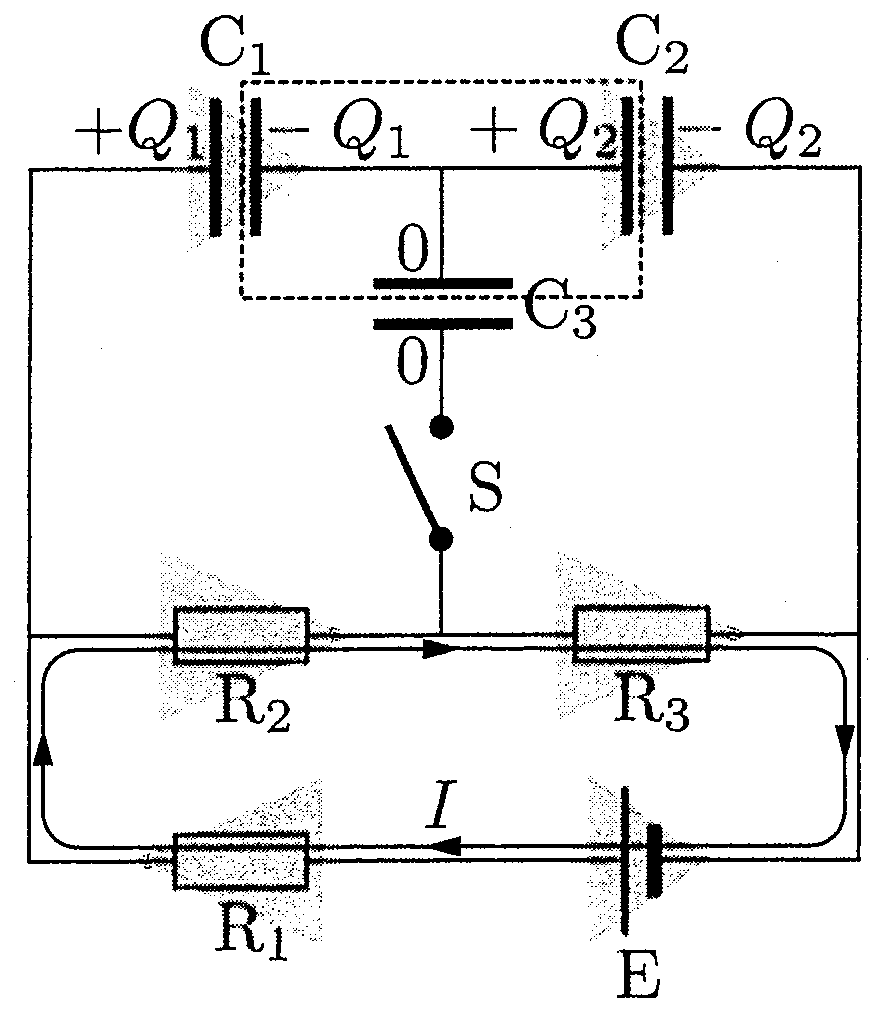
\includegraphics[keepaspectratio,width=52mm]{fig/n27_a76_zu1.png}\end{center}
       よってこの回路に対してキルヒホッフの第二法則を用いると，
       \[\begin{aligned}
         &\text{下側ループ：}\ 12=4\cdot I+8\cdot I+12\cdot I\\
         &\text{上側ループ：}\ 0=12\cdot I+8\cdot I-\frac{Q_1}{1}-\frac{Q_2}{3}
       \end{aligned}\]
       となるので，これを解いて，
       \[I=0.50\U{A}\Ans\]
       \begin{chuu}
       スイッチ$\mathrm{S}$が開いているので，左上のループおよび右上のループに対してはキルヒホッフの第二法則の式を立てることはできない．
       \end{chuu}
\ko{2} また，点線内部は電気的に浮いている部分であるから総電荷が保存される．もともとコンデンサーは帯電していなかったのだから総電荷量は$0$である．よって，
       \[0=-Q_1+Q_2+0\]
       が成立する．これと(1)のキルヒホッフの第二法則を組み合わせて解くと，$Q_1=Q_2=7.5\U{C}$であるから，コンデンサー$\mathrm{C}_1$の帯電量は
       \[Q_1=7.5\U{C}\Ans\]
\ko{3} スイッチ$\mathrm{S}$を閉じた場合にはコンデンサー$\mathrm{C}_3$の下側極板にも電流が流れ込むので電荷が溜まることになる．しかし定常状態ではどのコンデンサーにも電流が流れ込まなくなるので，電流は下側のループ部分のみで流れる．この電流を$I\U{A}$とし，コンデンサー$\mathrm{C}_1\sim\mathrm{C}_3$の帯電量をそれぞれ$\pm Q_1^\prime\sim\pm Q_3^\prime$とおくと，次図のような電流・電荷分布の図が描ける．
       \begin{center}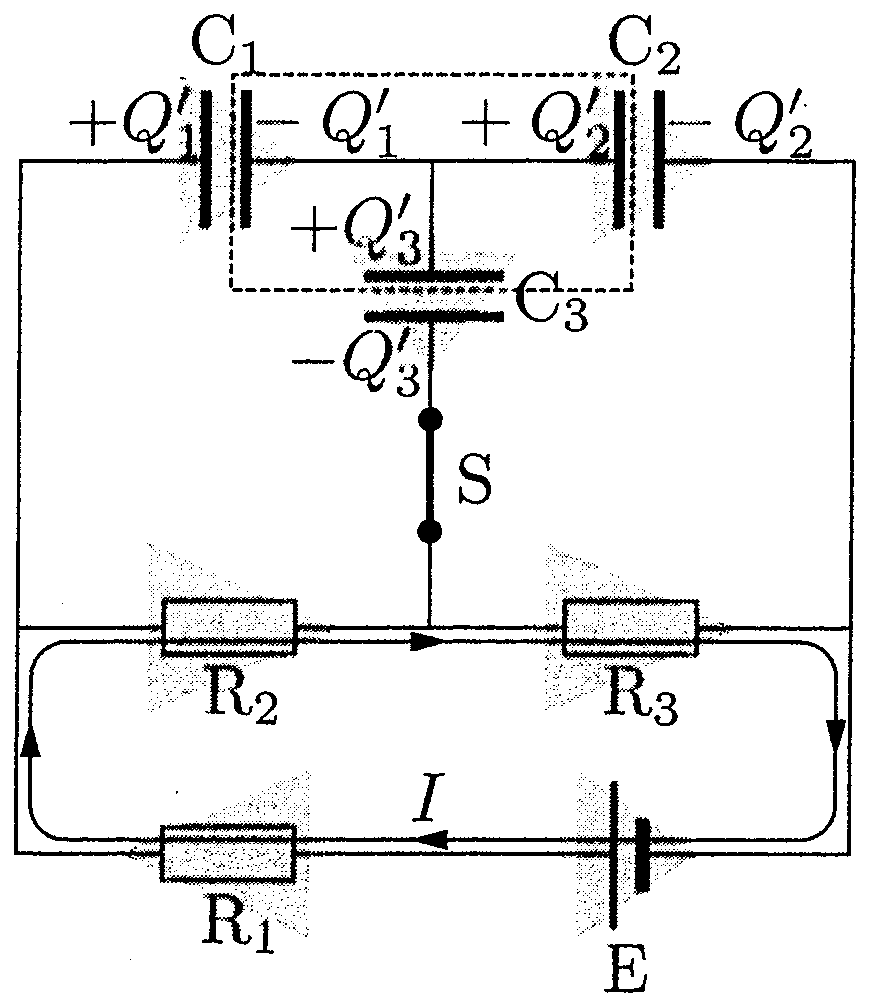
\includegraphics[keepaspectratio,width=52mm]{fig/n27_a76_zu2.png}\end{center}
       この回路に対してキルヒホッフの第二法則を用いて立式すると，
       \[\begin{aligned}
         &\text{下側ループ：}\ 12=4\cdot I+8\cdot I+12\cdot I\\
         &\text{左上ループ：}\ 0=8\cdot I-\frac{Q_1^\prime}{1}-\frac{Q_3^\prime}{10}\\
         &\text{右上ループ：}\ 0=12\cdot I+\frac{Q_3^\prime}{10}-\frac{Q_2^\prime}{3}
       \end{aligned}\]
       となる．また，点線内部は総電荷が保存される．もともとコンデンサーは帯電していなかったのだから総電荷量は$0$である．よって，
       \[-Q_1^\prime+Q_2^\prime+Q_3^\prime=0\]
       が成立する．以上四つの式を解いて，
       \[\begin{aligned}&I=0.50\U{A},\quad Q_1^\prime=5\U{C},\\ &Q_2^\prime=15\U{C},\quad Q_3^\prime=-10\U{C}\end{aligned}\]
       となる．よって，コンデンサー$\mathrm{C}_3$の上側極板には$+Q_3^\prime=-10\U{C}$の電荷が，また下側極板には$-Q_3^\prime=+10\U{C}$の電荷が蓄えられていることになるので，コンデンサー$\mathrm{C}_3$の帯電量は
       \[10\U{C}\Ans\]
\end{komon}

\MonN[\Sitei]{77}{非オーム抵抗}\par\nopagebreak
\begin{sisin}
与えられているグラフは，1個の電球に関して，かかる電圧$V$と流れる電流$I$との関係を示したものであるから，グラフと連動させるためには，あくまで1個の電球にかかる電圧を$V$，流れる電流を$I$，というふうに置かなければならない．幸いにして，(1)の回路では電球が直列接続されているので流れる電流が同じになり，かかる電圧も同じになる．また，(2)の回路では電球が並列接続されているのでかかる電圧が同じになり，流れる電流も同じになる．よって，回路中で設定しなければならない未知数は，1個の電球に関しての$V$，$I$のみで済む．

電球のような非オーム抵抗も，抵抗には変わりがないので，電流の向きと電圧の向きとの関係は通常の抵抗の場合と同様に考えればよい．
\end{sisin}
\KaiHead
\begin{komon}
\ko{1} 二つの電球は直列接続されているので，流れる電流は等しくなる．よってこれを$I\U{A}$とおく．流れる電流が同じであれば，各電球にかかる電圧も同じであるはずであり，これを$V\U{V}$とおく．回路に流れる電流および各素子にかかる電圧は次図のようになる．
       \begin{center}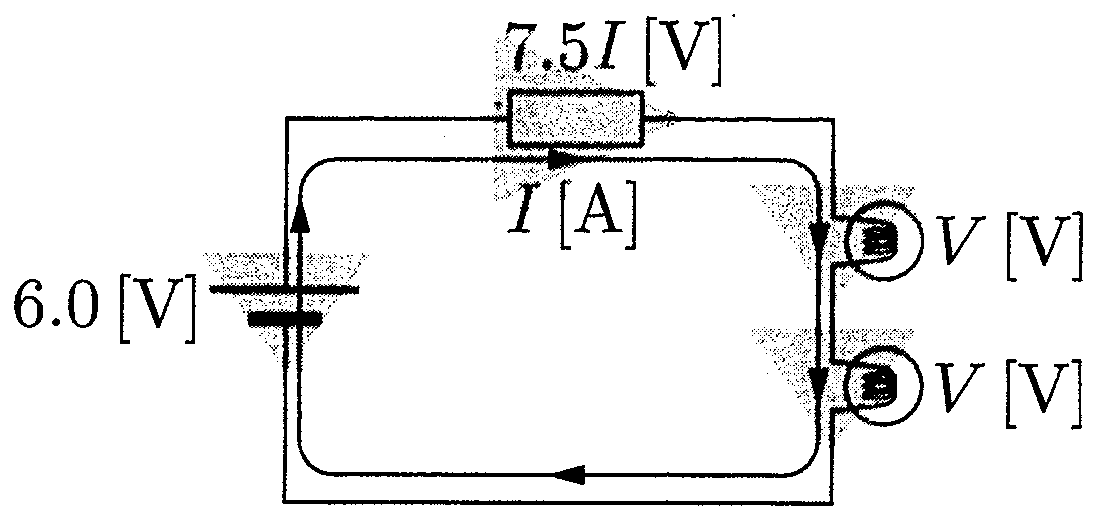
\includegraphics[keepaspectratio,width=52mm]{fig/n27_a77_zu1.png}\end{center}
       この回路にキルヒホッフの第二法則を用いると，$6.0=7.5\cdot I+V+V$と立式でき，これを解くと，
       \[1=\frac{I}{0.8}+\frac{V}{3}\]
       となる．上の式の関係をグラフ中に記入して交点を取ると，
       \begin{center}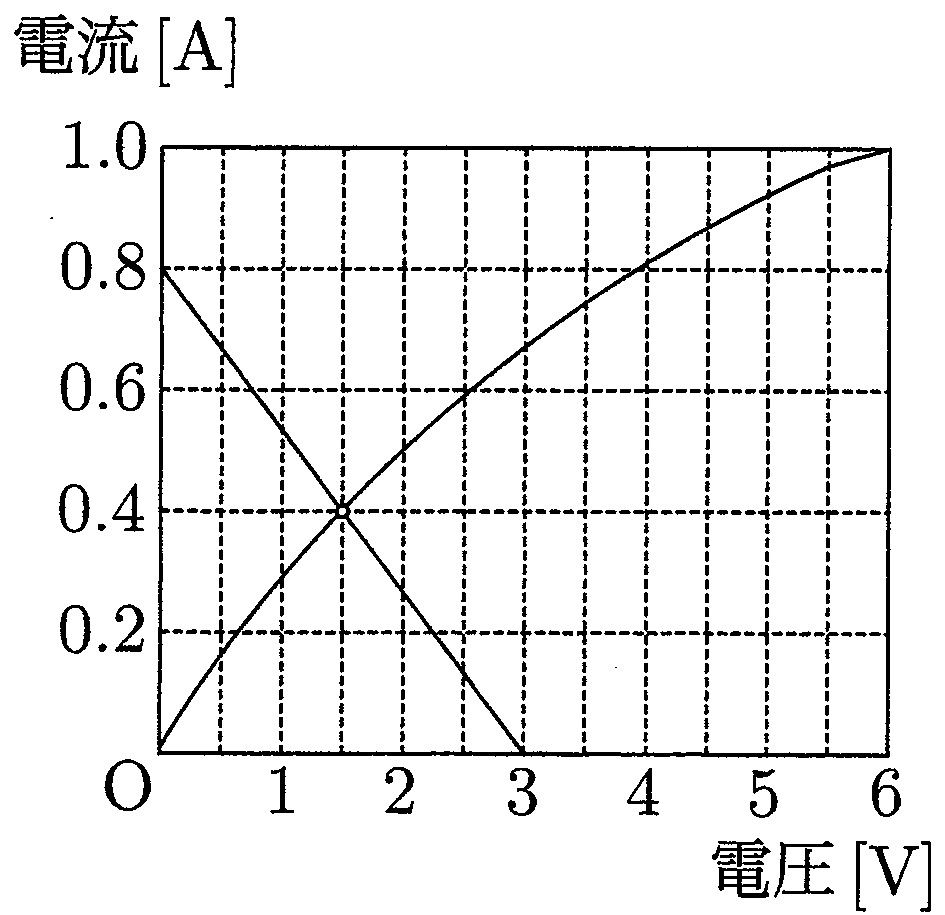
\includegraphics[keepaspectratio,width=46mm]{fig/n27_a77_graph1.png}\end{center}
       となるので，$V=1.5\U{V}$，$I=0.4\U{A}$となる．回路図より，抵抗を流れる電流の強さは，
       \[I=0.4\U{A}\Ans\]
\ko{2} 二つの電球は並列接続されているので，かかる電圧は等しくなる．これを$V\U{V}$とおく．かかる電圧が同じであれば，各電球を流れる電流も同じになるはずであり，これを$I\U{A}$とおく．回路に流れる電流および各素子にかかる電圧は次図のようになる．
       \begin{center}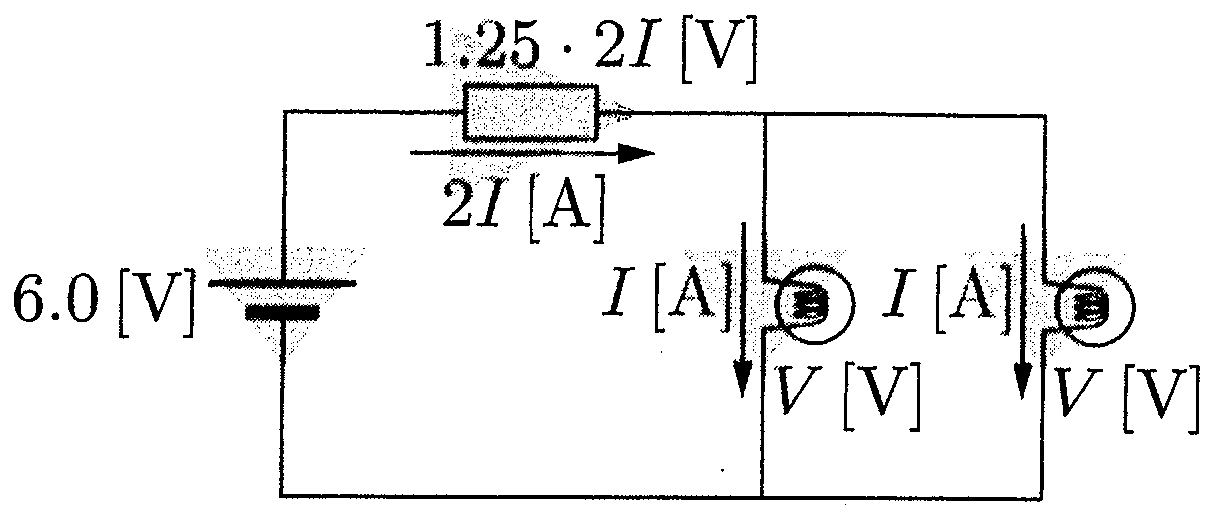
\includegraphics[keepaspectratio,width=56mm]{fig/n27_a77_zu2.png}\end{center}
       この回路にキルヒホッフの第二法則を用いると，左側ループに対して$6.0=1.25\cdot 2I+V$であり，これを解くと，
       \[1=\frac{I}{2.4}+\frac{V}{6.0}\]
       となる．上の式の関係をグラフ中に記入して交点を取ると，$V=4.0\U{V}$，$I=0.8\U{A}$．
       \begin{center}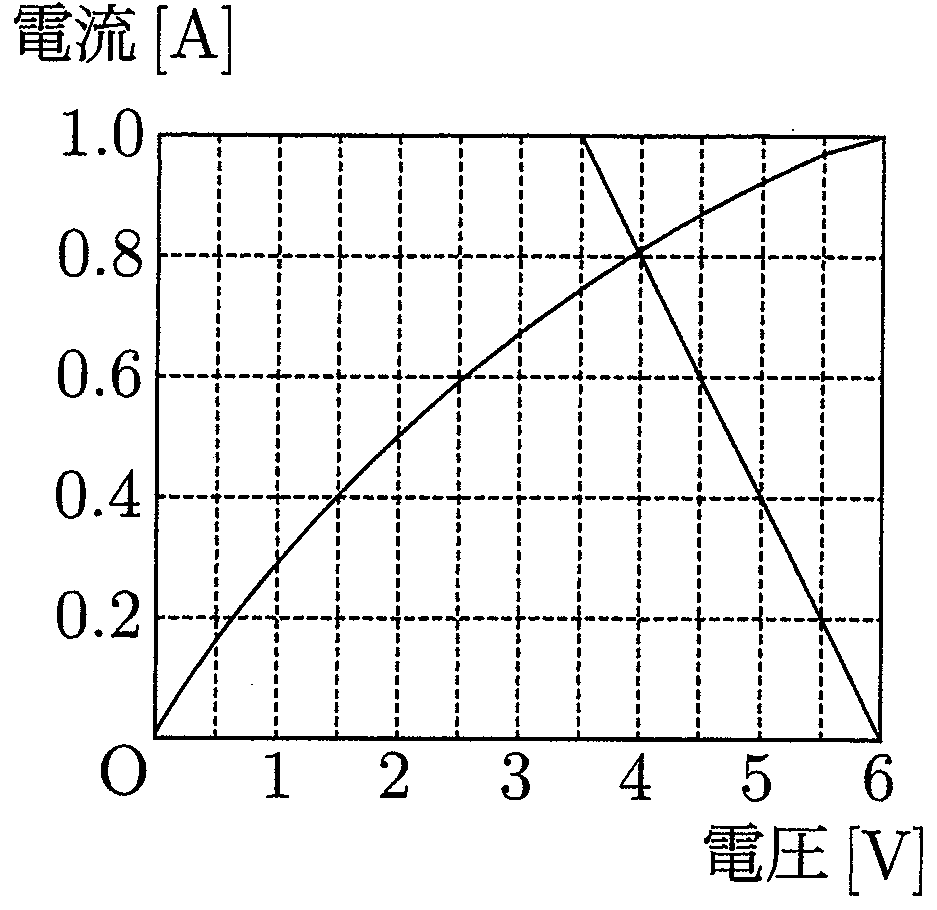
\includegraphics[keepaspectratio,width=46mm]{fig/n27_a77_graph2.png}\end{center}
       回路図より，抵抗を流れる電流の強さは$2I\U{A}$であるから，
       \[2I=1.6\U{A}\Ans\]
\end{komon}

\Rank{C問題}
\MonN{78}{非オーム抵抗の組み合わせ}\par\nopagebreak
\begin{sisin}
電球$\mathrm{A}$，$\mathrm{B}$が並列・直列接続されていることに着目して，この二つを一つの電球としてまとめてしまい，合成した上で考える（27.5）．
\end{sisin}
\KaiHead
\begin{komon}
\ko{1} 電球$\mathrm{A}+\mathrm{B}$を一つの素子とみなし，この素子に対して電圧$V\U{V}$をかけたときに流れる電流$I\U{A}$を考える．電球$\mathrm{A}$，$\mathrm{B}$は並列接続されているので，$I$は電球$\mathrm{A}$，$\mathrm{B}$それぞれ流れる電流の和$I_{\mathrm{A}}+I_{\mathrm{B}}$になる．よって，この合成素子の$I$-$V$特性曲線は，二つのグラフを縦方向に足し合わせることによって得られる．
       \begin{center}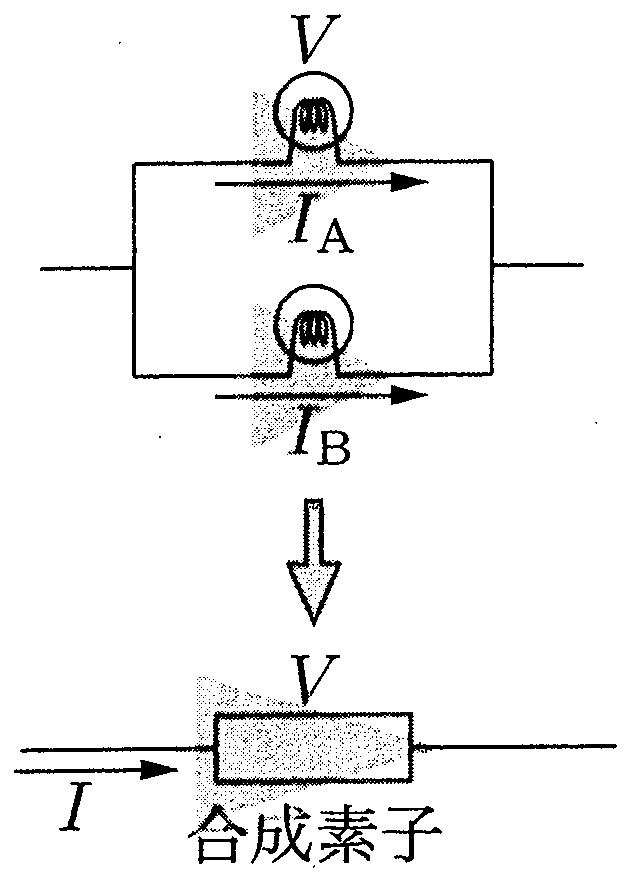
\includegraphics[keepaspectratio,width=26mm]{fig/n27_a78_zu1.png}\hspace{4mm}%
       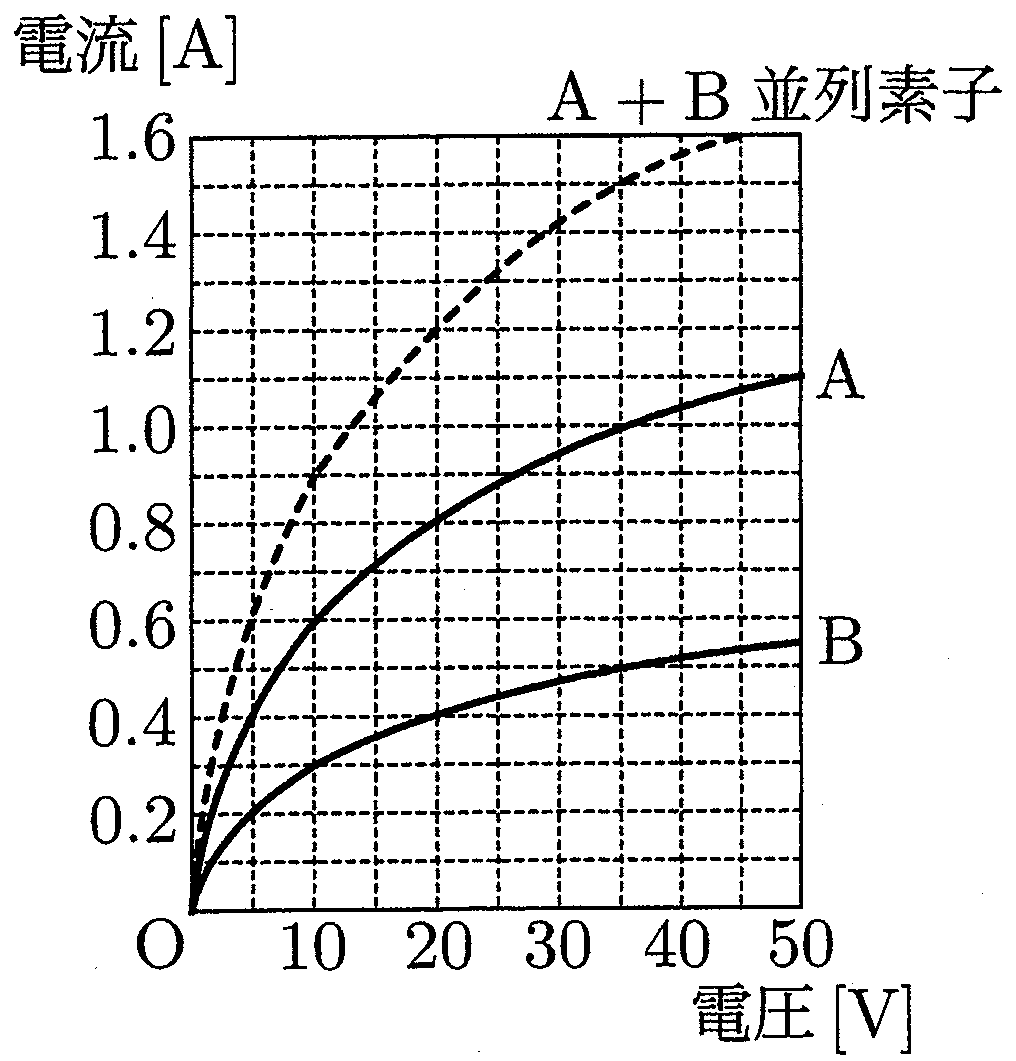
\includegraphics[keepaspectratio,width=40mm]{fig/n27_a78_graph1.png}\end{center}
       この合成素子にかかる電圧，および流れる電流を$V\U{V}$，$I\U{A}$とおくと，この回路は次図のようにみなせる．
       \begin{center}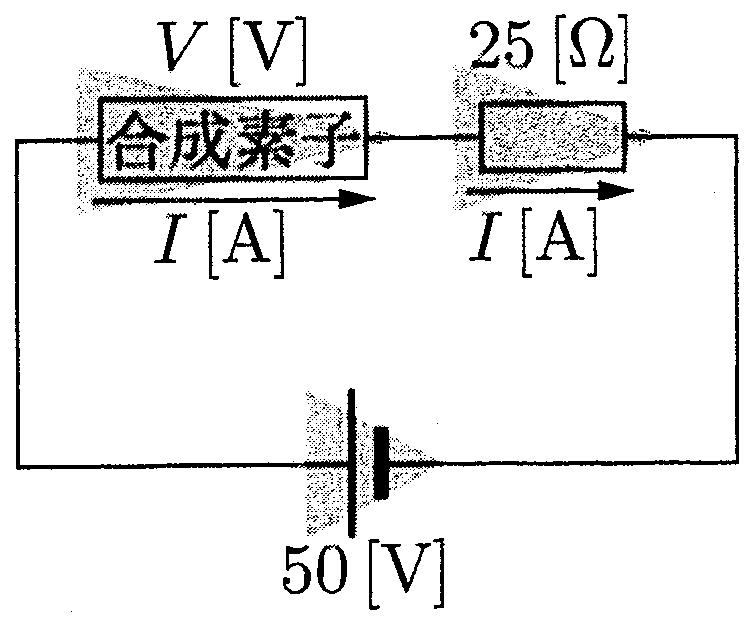
\includegraphics[keepaspectratio,width=40mm]{fig/n27_a78_zu2.png}\end{center}
       キルヒホッフの第二法則より，$50=V+25\cdot I$であり，これを解いて
       \[1=\frac{V}{50}+\frac{I}{2}\]
       であるから，これを$\mathrm{A}+\mathrm{B}$並列合成素子の$I$-$V$特性曲線に記入して交点を取ると，$I=1.2\U{A}$，$V=20\U{V}$．
       \begin{center}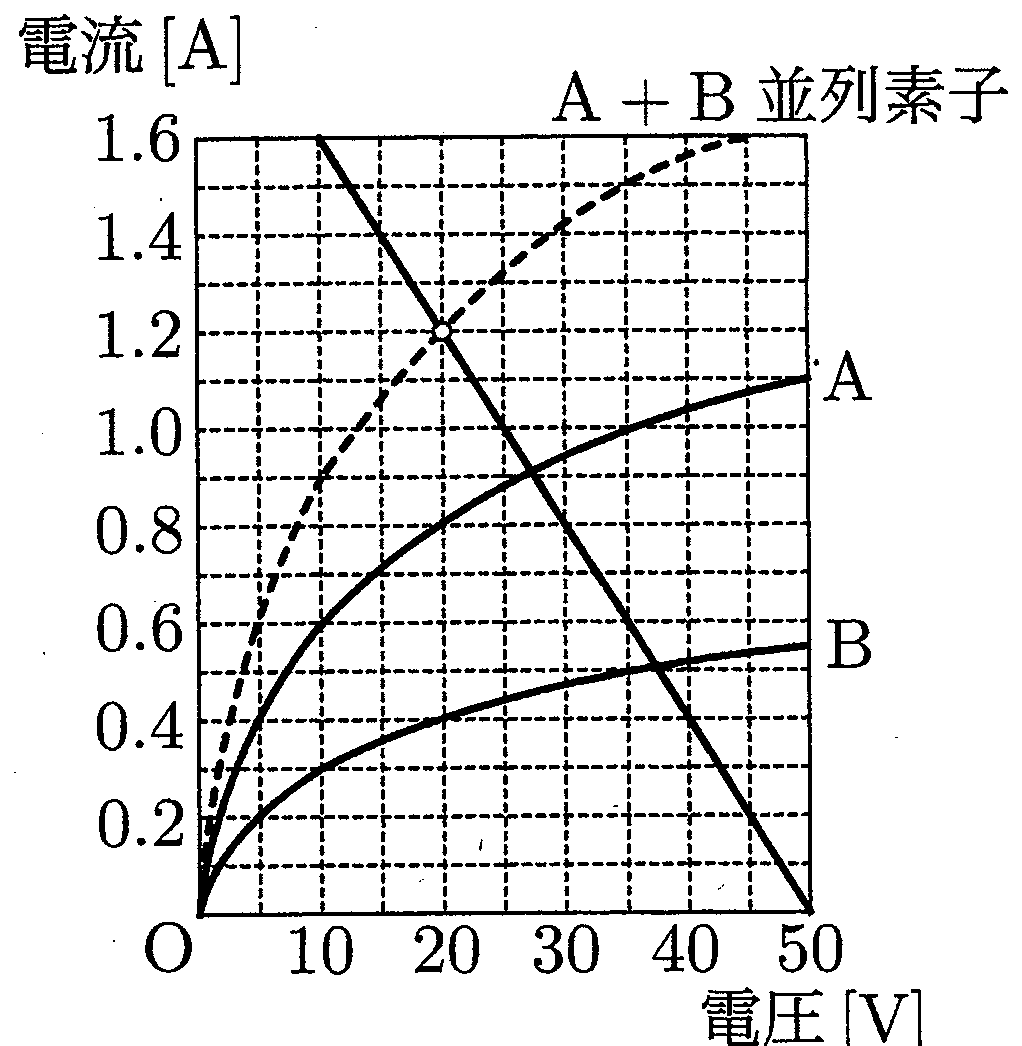
\includegraphics[keepaspectratio,width=44mm]{fig/n27_a78_graph2.png}\end{center}
       抵抗を流れる電流は$I\U{A}$であるから，
       \[I=1.2\U{A}\Ans\]
\ko{2} 電球$\mathrm{A}+\mathrm{B}$を一つの素子とみなし，この素子に対して電流$I\U{A}$を流したときの両端間の電圧$V\U{V}$を考える．電球$\mathrm{A}$，$\mathrm{B}$は直列接続されているので，$V$は電球$\mathrm{A}$，$\mathrm{B}$それぞれにかかる電圧の和$V_{\mathrm{A}}+V_{\mathrm{B}}$になる．よって，この合成素子の$I$-$V$特性曲線は，二つのグラフを横方向に足し合わせることによって得られる．
       \begin{center}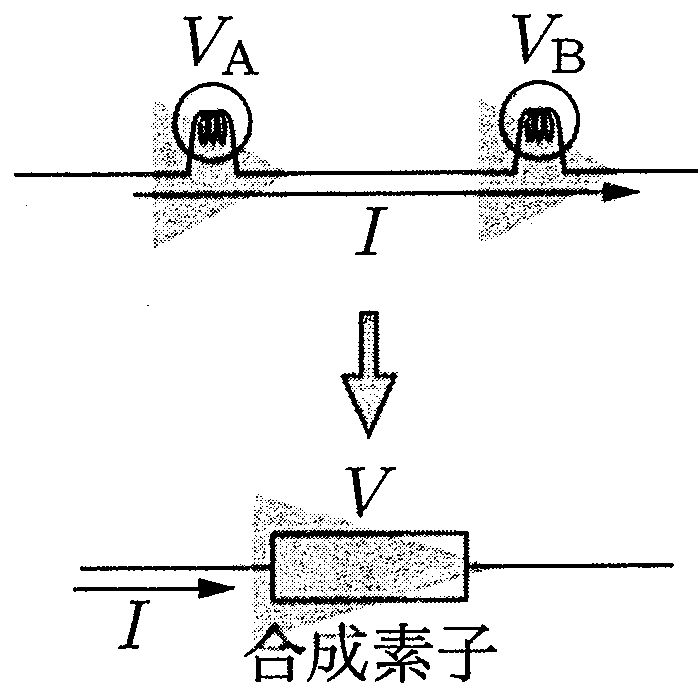
\includegraphics[keepaspectratio,width=30mm]{fig/n27_a78_zu3.png}\hspace{4mm}%
       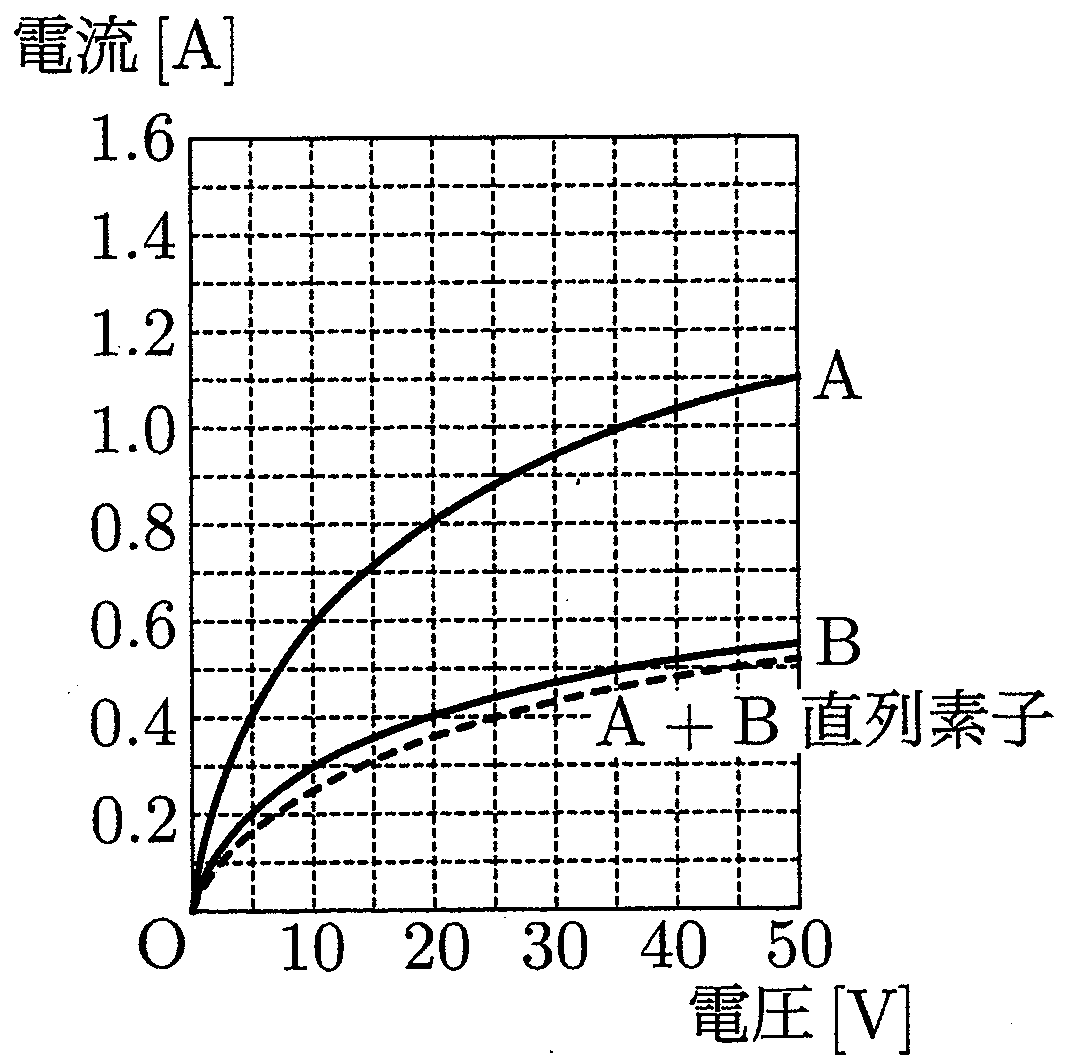
\includegraphics[keepaspectratio,width=40mm]{fig/n27_a78_graph3.png}\end{center}
       この合成素子にかかる電圧，および流れる電流を$V\U{V}$，$I\U{A}$とおくと，この回路は次図のようにみなせる．
       \begin{center}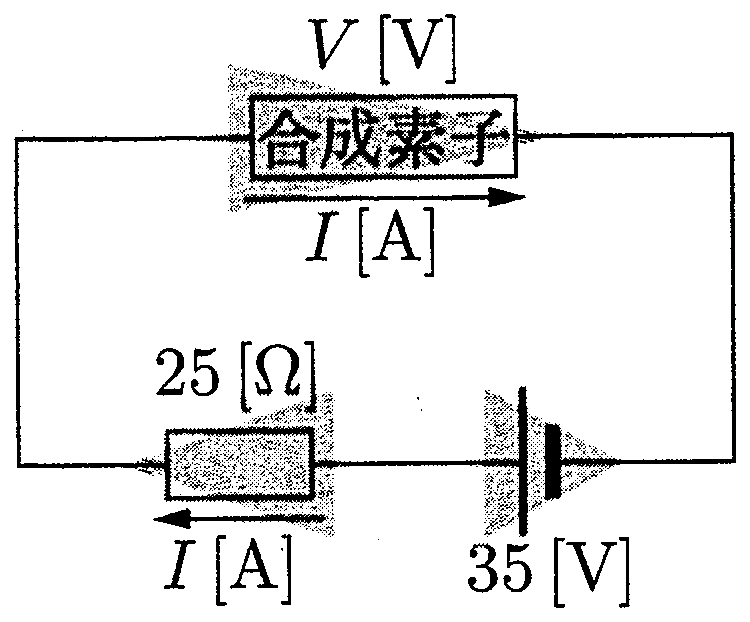
\includegraphics[keepaspectratio,width=36mm]{fig/n27_a78_zu4.png}\end{center}
       キルヒホッフの第二法則を用いて，$35=V+25\cdot I$であり，これを解いて
       \[1=\frac{V}{35}+\frac{I}{1.4}\]
       であるから，これを$\mathrm{A}+\mathrm{B}$直列合成素子の$I$-$V$特性曲線に記入して交点を取ると，$I=0.4\U{A}$，$V=25\U{V}$．
       \begin{center}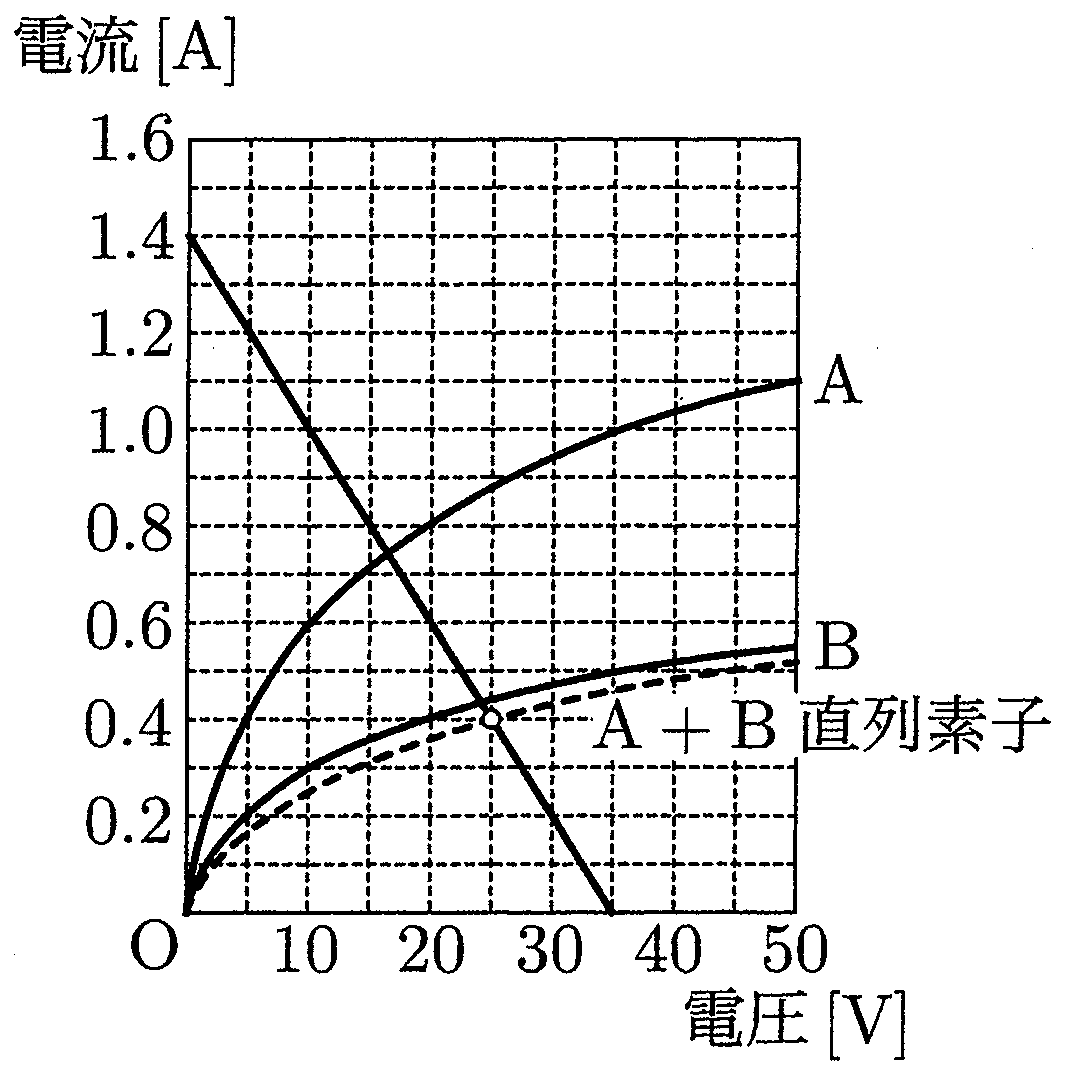
\includegraphics[keepaspectratio,width=44mm]{fig/n27_a78_graph4.png}\end{center}
       抵抗を流れる電流は$I\U{A}$であるから，
       \[I=0.4\U{A}\Ans\]
\end{komon}

\MonN{79}{抵抗値}\par\nopagebreak
\begin{sisin}
{\gtfamily 非オーム抵抗の抵抗値は，その瞬間にかかっている電圧と流れている電流の比}として与えられる（27.5）．
\end{sisin}
\KaiHead
このときの電球の抵抗値を$R\U{\Omega}$とすると，検流計$\mathrm{G}$に電流が流れないとき，ブリッジの平衡条件より
\[32:12=20:R\]
が成立する．これを解いて，$R=7.5\U{\Omega}$である．よって，電球にかかっている電圧$V\U{V}$と流れる電流$I\U{A}$との間に
\[7.5=\frac{V}{I}\]
が成立する．グラフ上でこれを満たす点をさがすと，$I=1.6\U{A}$，$V=12\U{V}$．よって，このとき電球に流れている電流は，
\[I=1.6\U{A}\Ans\]
\begin{center}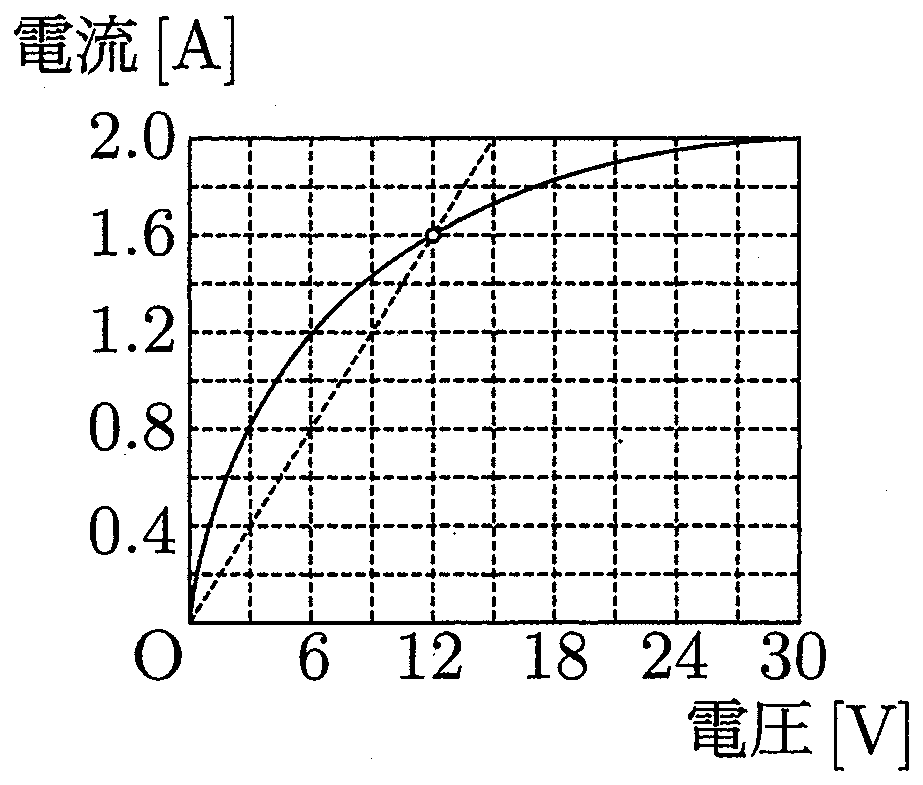
\includegraphics[keepaspectratio,width=44mm]{fig/n27_a79_graph.png}\end{center}

\MonN{80}{ダイオード}\par\nopagebreak
\begin{sisin}
ダイオードに関する問題は，大きく分けると\MARU{1}本問のように$I$-$V$特性曲線が与えられてそれを用いて考えさせる問題と，\MARU{2}コンデンサーのスイッチ切り替え問題に組み込んで，ある一方向にしか電荷を流さない特殊素子として利用するタイプの問題の2通りがある．前者の場合には，単なる非オーム抵抗として問題を解けばよい（27.6）．
\end{sisin}
\KaiHead
\begin{komon}
\ko{1} 回路にキルヒホッフの第二法則を用いると，次図を参照して，
       \begin{center}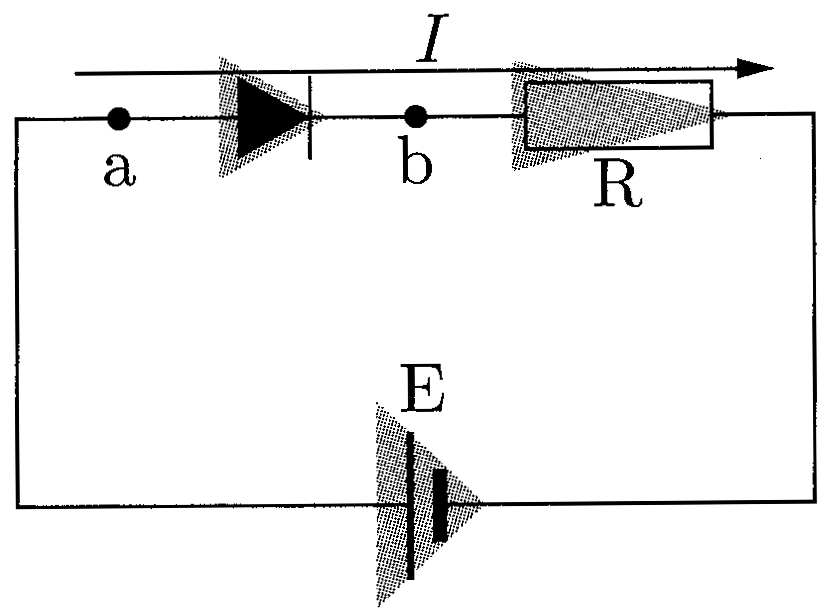
\includegraphics[keepaspectratio,width=40mm]{fig/n27_a80_zu1.png}\end{center}
       \[E=V+RI\Ans\]
\ko{2} $E=5\U{V}$，$R=5\U{\Omega}$を代入すると，
       \[\frac{V}{5}+\frac{I}{1}=1\]
       となり，これをグラフ中に記入して交点を取ると，
       \[V=1.0\U{V},\qquad I=0.8\U{A}\Ans\]
\ko{3} 電池を反転させた場合の回路は次図のようになる．
       \begin{center}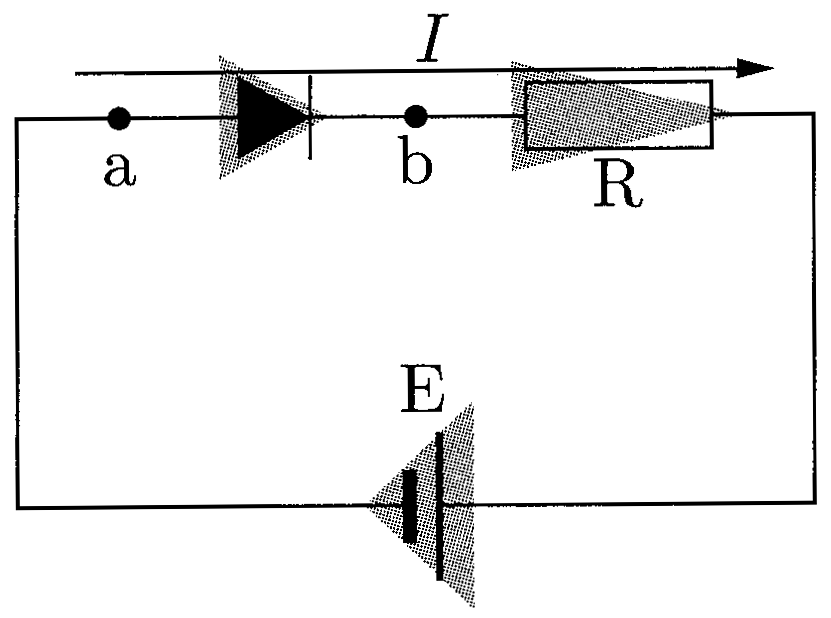
\includegraphics[keepaspectratio,width=40mm]{fig/n27_a80_zu2.png}\end{center}
       キルヒホッフの第二法則を用いて，
       \[E=-RI-V\Ans\]
\ko{4} $E=5\U{V}$，$R=5\U{\Omega}$を代入すると，
       \[\frac{V}{-5}+\frac{I}{-1}=1\]
       となり，これをグラフ中に記入して交点を取ると，
       \[V=-4.5\U{V},\qquad I=-0.1\U{A}\Ans\]
\end{komon}
\begin{bsHosoku}{参考}
これらの(2)，(4)から，ダイオードに対して逆方向に電池をつないでも電流はほとんど流さないことが分かる．ダイオードはこのように電流の流れを制御することができるので，整流素子として利用される．
\end{bsHosoku}

\end{multicols}
